\documentclass[preprint, 12pt]{elsarticle}

% Options
\biboptions{longnamesfirst, authoryear}

% KU requirements
\usepackage[margin=2.5cm]{geometry}
\usepackage{setspace}
\onehalfspacing

% Temporary packages used while editing
\usepackage[usenames,dvipsnames]{color}

% Packages

\usepackage[colorlinks=true]{hyperref}
\usepackage{xspace}
\usepackage[utf8]{inputenc}
\usepackage{listings}
\usepackage{caption}
\usepackage{subcaption}
\usepackage{graphicx}
\usepackage{picins}
\usepackage{rotating}



% CUSTOM COMMANDS
\newcommand*{\TODO}{\textbf{\fbox{??}}}%

%% Note and Source below tables and figures
\usepackage{threeparttable} % Alternative for Notes below table
\newcommand{\Figtext}[1]{%
	\begin{tablenotes}[para,flushleft]
		\hangindent=1em
		\footnotesize
		\raggedright
		#1
	\end{tablenotes}
}
\newcommand{\Fignote}[1]{\Figtext{\emph{Note:~}~#1}}
\newcommand{\Figsource}[1]{\Figtext{\emph{Source:~}~#1}}

%%%%%%%%%%%%%%%% TO-DO: replace \TODO %%%%%%%%%%%%%%%%%%

\begin{document}

\pagenumbering{gobble}
%\clearpage

\begin{frontmatter}

\title{Competitive location behaviour with foresight}
\author{Jonas K. Sekamane}
\journal{Supervised by Johan Lagerlöf.}

\begin{abstract}
{...}
\end{abstract}

\end{frontmatter}

% Table of contents
\singlespacing
%\setcounter{tocdepth}{2}
\makeatletter
	\@starttoc{toc}
\makeatother
\onehalfspacing

\newpage
\clearpage
\pagenumbering{arabic}

%% main text
\section{Introduction}

In the field of economics, competition is often synonymous with price competition. However businesses compete with one another on a multitude of other factors. Retailers compete for customers when they choose their location. Manufacturers compete when they choose product characteristics such as size, colour, shape, style, flavour, etc. 

The range of available products is a response to the diversity of consumer preferences. Specific products and specific locations are selected to appeal to different segments of the market. Consumers have idiosyncratic preferences over their preferred variant. Some prefer a sweeter cider to a more sour cider, and vice versa. Similarly consumers favour shops located in their respective neighbourhood over shops located in other neighbourhoods. This inherent heterogeneity among individuals creates a collective demand for product diversity and a demand across all neighbourhoods. Consequently consumers are willing to pay more for variants that better mirror their preferences. These premiums open up for the possibility that firms maintain a price level above marginal costs and are thus a source of market power.

The market is unlikely to sustain a large number of products or retailers -- even with broad diversity in consumer preferences -- because of increasing returns to scale in production, distribution, R\&D, etc. Each firm must capture a sufficiently large share of the market to cover its fixed costs. This in turn creates a natural barrier that prohibits each individual consumer from simply producing his or her preferred product. Instead the market will consist of few firms that compete with one another for customers. With few firms in the market it is hard to defend the assumption of \emph{competitive price-taking} firms, or similar assumptions that treat firms as identical passive entities. Instead competition and interaction among firms is strategic. When a profit-maximising firm evaluates different actions -- such as its location or product characteristics -- it should take account of the potential demand associated with each action. The firm plays an active role in shaping its outcome and can appeal to different segments through its choices. Additionally firms with foresight should consider the action and response from competing firms. If all competitors are contemplating opening a shop on Main Street, then the retailer might secure a larger profit by locating off Main Street despite the lower concentration of consumers there. It is not enough that the action of the firms is profitable given the current state. The firms compete for the same consumers, therefore the long-term profitability is contingent on the firm's ability to predict the future action of competing firms and respond accordingly. This may include, but is not limited to, finding a niche segment of the market that is sufficiently large to sustain the firm, or engaging in direct competition while maintaining the flexibility to adjust to changes.

The natural setting when considering competitive location or competitive product differentiation is a market with few firms where firms act strategically and with foresight. The choice of each firm reflects the diversity of consumer preferences and so the aggregated distribution of consumer preferences is likely to be of great importance. Moreover the aggregated distribution of each consumer's preferred product or location does not necessarily follow a convenient uniform, symmetric or even unimodal distribution. The distribution may well be asymmetric and multi-modal.

This type of competition has received fare less attention than price competition, and consequently many important questions have yet to be answered. Most notably what happens when multiple firms compete in a multidimensional space. For instance several retailers locating in a two-dimensional geographic space, or multiple cider producers considering product differentiation along several dimensions such as sweet-sour, sparkling-still, clear-cloudy etc. Every day business owners make decisions in settings such as these. And yet the literature on economics lack a solid theoretical understanding of how firms make these decisions and how it affects the overall market. In light of this it seems evident that product differentiation is a crucial factor missing in our understanding of how modern market economies operate.

This paper will be purely theoretical. It does not aim to provide business owners with best practices on how to locate nor how to differentiate itself from competitors. The aim is to understand the decision process of firms. This requires developing a theoretical model capable of analysing the decisions, yet versatile enough to handle the settings firms often find themselves competing in (i.e. few firms acting strategic with foresight in a market not necessarily restricted to a single dimension and where the distribution of consumer preferences might be asymmetric and multi-modal). The development of a theoretical model opens the future field of study to more practical applications and analyses. One such analysis might concern the above mentioned market power that arises from consumers willingness to pay a premium for product variants that better reflect their preferences. If this severely distorts the market, then antitrust and competition laws should take account of it. Another analysis might concern the additional source of market failure that can arise from the selection process. When firms compete through their choice of product characteristics or location, it may lead to an under- or oversupply. Unique to models, where the product selection is endogenous, is also the possibility that competition leads to the wrong products or locations. For instance competition among retailers may lead all retailers to locate in the city centre, even if the socially optimal locations is one where retailers are evenly dispersed across the neighbourhoods of the city. If this is the case, the government or local zoning laws should adjust incentives so firms choose efficient locations and the efficient set of products from the spectrum of possible variants.

Models studying this type of competition are collectively known as \emph{competitive location models}. The first was Hotelling's line market, where two firms compete for consumers that are evenly distributed along one dimension \citep{Hotelling_1929}. The model has been extended in numerous ways, such as the number of firms, the distribution of consumers, and the number of dimensions. The traditional approach has been to solve for the equilibria of the model analytically. The conclusions then follow from analysing these equilibrium settings. The limited number of new insights discovered the last 15 years, suggests that this approach might be reaching its limits. \citet[p.~869]{Biscaia_Mota_2013} write that \emph{``it would seem that most of the important features that justify the spatial behaviour of firms have already been explored''}. In addition it has been proven that some location models -- despite being fairly simple in their setup -- belong to a set of problems suspected to be infeasible to solve. An alternative approach to these types of models, recently advanced in the political science literature, rely on agent-based modelling. The location problem is set up as a computer model in which the agents act simultaneously and according to a given set of decision rules. The model is analysed by running the simulation and observing how the interaction of agents play out. The agent-based model allows researchers to study settings that are beyond the reach of the analytical approach. In the current models agents act using simple rules of thumb or heuristics without any type of foresight. That is, each agent is oblivious to the future behaviour of the other agents and does not take their behaviour into account when deciding its own location. The agent-based models developed so far lack the strategic considerations fundamental to earlier competitive location models.

This paper uses the agent-based model laid out by \citet{Laver_Sergenti_2011}. We construct a new decision rule with foresight. With this rule the firm forecasts the future location of competing firms and uses the predicted locations when it decides where to locate. The forecast method used in this paper is a modified version of the one advanced by the \emph{Santa Fe Artificial Stock Market} model \citep[chapter~11]{Arthur_2014}. With this method firms use \emph{inductive reasoning}, i.e. they hold several hypotheses on how a competing firm chooses to locate and use the most accurate hypothesis that fits the current state to predict the future location. The firm gradually discard poorly performing hypotheses and form new hypotheses. The model is dynamic and firms act simultaneously. The results of the model are derived by observing how the interaction of firms play out.

In this paper we disregard price competition and focuses solely on the type of competition that takes place through product differentiation or location differentiation. While disregarding price competition leaves much to be desired in terms of developing a unified and fundamental theoretical model, it reduces the complexity of the model significantly. We leave it up to future research to appropriately incorporate price competition and determine its effect on the results. In the models we assume that all firms charge the same fixed price. A situation like this might arise because of government regulation, or if firms previously committed themselves to a fixed price. The situation may also arise if firms are subject to a \emph{retail price maintenance} agreement, where prices are fixed earlier in the distribution channel, e.g. by manufacturers or wholesalers. To make the paper easier to read and for the sake of consistency the models are formulated in terms of geographic location. However the results also apply to product differentiation and in the context of political parties competing for voters through their choice of policy positions.

\TODO{summarise results ... it is a colossal task. The paper does not provide answers to all questions. But it is a first step in developing a model where foresight and strategic considerations are integral to the decision process ... }

The paper is structured as follows. The literature review covers previous results from competitive location models such as Hotelling's line market, its extensions, and the agent-based model. This section also covers research on related concepts that are used in later sections, such as Voronoi diagrams, distance metrics and implementation of learning in economic models. The final model is quite complex. To aid the reader the paper gradually introduces decision rules and adds layers to the model, starting with the most simple. The model and basic decision rules without foresight are introduced in the methodology sections. The section discusses the approach used to solve the model and estimate the output values of the model. In addition the section presents methods on how to parameterise the model and determine when the model has \emph{burnt in}, such that the results obtained are independent of the initial position of firms. The analysis section presents the results of the models where firms make decisions without foresight, followed by a detailed introduction of the decision rule where firms use \emph{inductive reasoning}, and finally the results from this decision rule.


\section{Literature review}

The literature on spatial competition began with \citeauthor{Hotelling_1929}'s \citeyearpar{Hotelling_1929} paper. Hotelling proposes a line market where consumers are uniformly distributed along the line and firms produce identical goods. Consumers inelastically demand one unit from the firm with the lowest price. The price is composed of the \emph{mill price} and \emph{transportation cost}. Each firm charges a \emph{mill price}, i.e. the price for one unit purchased at the doorsteps of the firm. And customers bear a cost by going to the firm to shop. This \emph{transport cost} is linear in the distance between the customer and the firm. Two firms decide where to locate and which \emph{mill price} to charge. Firms first simultaneously choose their location, and thereafter simultaneously decide on their prices. Two opposing forces come into play; If the firm locates close to its competitor, it will attract more consumers. Meanwhile locating closer also lead to more fierce price competition from its competitor.

If \emph{mill prices} are fixed and equal then there is no price competition and both firms locate at the centre of the market and split the market equally. The agglomeration of firms has been coined the \emph{principle of minimal differentiation}\footnote{The\emph{principle of minimal differentiation} was coined by Boulding in 1955 \citep{Biscaia_Mota_2013}.}. The average distance travelled by consumers is one-fourth the length of the line. This is socially suboptimal. The social optimal location is where the market is split in two equal halves, with a firm located at the centre in each of these halves. This reduces the average distance travelled by consumers to one-eighth of the length of the line. 

An error lead Hotelling to conclude that the model with price competition would also exhibit the \emph{principle of minimal differentiation}. But when two firms are located close to each other near the centre, price competition drives down prices to a level where it is no longer optimal for firms to locate in the middle half of the line. The paper by \citet{dAspremont_Gabszewicz_Thisse_1979} shows this and that no equilibrium exists in the model laid out by Hotelling. Instead they modify \emph{transportation cost} to be quadratic in the distance between the customer and the firm, rather than linear. With this modification a unique equilibrium exist, but where firms locate at either ends of the line, i.e. \emph{maximal differentiation}. This shows how the \emph{principle of minimal differentiation} breaks down when price competition is introduced. Unfortunately it is just one of many examples of how sensitive the conclusions from the Hotelling model are to changes in the setup. 

Below I will review some of the literature on the Hoteling model and more generally spatial competition models. I will present the reader with papers that relax the assumptions and generalise the Hotelling model. \citet{Biscaia_Mota_2013} find 352 published journal articles since 1979 that reference `Hotelling' or `spatial competition'. The sheer volume of papers on the topic makes it a colossal task to provide an exhaustive review. This literature review is not exhaustive, but selective and focused on the papers deemed relevant for this particular paper. The following set of papers provide an exhaustive review of the topic; The early developments and historical development of the spatial competition literature is reviewed by \citet[chapter~1]{Eiselt_Marianov_2011} and \citet{Smith_Laporte_Harper_2009}. \citet{Biscaia_Mota_2013} contain a bibliometric analysis of the literature. \citet{Eiselt_2011} provide a reissue of Hotelling's original paper with comments and references to later contributions. \citet{Graitson_1982, Brenner_2001, Eiselt_Laporte_Thisse_1993} provide literature reviews focused on the Hotelling model. While \citet{Kilkenny_Thisse_1999} and \citet{ReVelle_Eiselt_2005} give a more general review of spatial competition models. \citet{Daskin_2008} provide a review of discrete spatial competition models. Sequential location models are reviewed by \citet{Eiselt_Laporte_1996} and \citet{Kress_Pesch_2012}. And the review by \citet{Plastria_2001} focuses on the optimisation approaches to competitive location models.

\subsection{Multiple firms and two-dimensional space}

\citet{Eaton_Lipsey_1975} considers both the line market and two-dimensional space. They assume that firms charge a fixed price, and they investigate the equilibrium with $N$ number of firms in the market. Where the number of firms is exogenously determined.

\citet{Eaton_Lipsey_1975} prove analytically that no equilibrium solution exists when three firms have similar prices. In the line market the two firms at each perimeter will move towards the centre of the line, reducing the market of the third firm. Eventually this forces the firm at the centre to leapfrog to the outside. This process continues with the two outer firms again moving towards the centre of the line. This has been referred to as the \emph{dancing equilibria} although it does not fulfil the requirements of an equilibrium \citep{Eiselt_2011}. In the line market with four firms, two firms will locate at one-fourth the length, and two firms will locate a three-fourths the length of the line. Similarly in the case of five firms, two firms are located at one-fifth the length, two at four-fifths the length, and the fifth firm locates at the centre. The equilibrium ceases to be unique for six or more firms, instead it is a range of equilibria. If there is an odd number of firms, then one firm will be located at the centre of the line. The firms on the perimeters are paired. While the remaining interior firms may be paired, or may be separated by some distance. However no firm has a total market area that is less than the largest \emph{half-market} of any other firm. The \emph{half-market} refers to the two market areas on either side of the firm. \citet{Eaton_Lipsey_1975} conjecture that the \emph{principle of minimum differentiation} should perhaps be replaced by the \emph{principle of local clustering}, since pairs of firms choose to locate close to one another. \citet{Eaton_Lipsey_1975} also consider multimodal and asymmetric distributions of consumers along the line. Here they prove that an equilibrium requires that the number of firms in the market does not exceed twice the number of peaks in the consumer density function, i.e. if the distribution of consumers is bimodal (two peaks), then no equilibrium exists with four or more firms in the market. 

The results above from \citet{Eaton_Lipsey_1975} rely on the assumption that firms behave without foresight -- referred to as \emph{zero conjectural variation}. \citet{Eaton_Lipsey_1975} drop this assumption to analyse how firms with foresight choose to locate. To do this they assume that firms adopt a \emph{minimax strategy} where firms anticipate the entry of a new firm into the market. This leads firms to minimise the size of their largest \emph{half-market}. When a firm locates at the centre of its own market, rather than at the perimeters, it minimises its exposure to new firms entering the market. With this assumption firms never locate in pairs as described above. Instead, for any number of firms, there exists a unique equilibrium where firms are evenly spaced along the line. These equilibria are socially optimal as they minimise the average distance to consumers. The \emph{principle of local clustering} no longer holds when firms use a \emph{minimax strategy}. Further note that the \emph{minimax strategy} does not consider whether or not entry is a rational strategy for new firms, and thus it leads to an inadequate equilibrium concept.

\citet{Shaked_1975} prove analytically that no equilibrium exists for three firms locating in the plane. \citet[p.~40]{Eaton_Lipsey_1975} note that it is not obvious how three or more firms will choose to locate in two-dimensional space, and write that \emph{``using conventional analytical techniques the problem is very complex, perhaps intractable''}. Instead they use simulation techniques and once again assume that firms behave without foresight. In their simulation consumers are uniformly distributed on a disc, rather than a square plane. With any number of firms between 3 and 17, they show that a local equilibrium exists for the firm, where all firms are evenly spaced along a circle with the same centre as the disc, and with a radius that is less than the radius of the disc. However this is not a global equilibrium, and the circular configuration immediately breaks up, since one firm will choose to pair up with one of its neighbours rather than remain fixed on the circle. The same is true with less than 9 firms in the market, where one firm is located at the centre, and the remaining firms are evenly spaced in a circular configuration. With 9 or more firms in the market, the firm at the centre is in a global equilibrium, but the firms on the circle are only in a local equilibrium. In addition they show that no equilibrium exists for firms located in a hexagonal pattern, square pattern or rectangular pattern. The firms at the perimeter of the market will pair up with neighbours, breaking these patterns. In sum they suspect that no equilibrium solution exists for three or more firms in two-dimensional space. \citet{Shaked_1975} proved their suspicion in the case with three firms. But it remains an open question with more than 3 firms in the market.

The general result -- from the 85 years of research since Hotelling published his paper -- is that conclusions and equilibrium are non-robust across alternative model specifications. Researchers have generalised the model, but most results are falsified when assumptions are modified. And even minor modification may remove any equilibrium constellations.

\subsection{Location problems}

The Hotelling model belongs to a wider set of \emph{competitive location models}, which again falls into the more general realm of \emph{location problems}. The difficulty of finding optimal solutions is not restricted to the Hotelling model. It shows up in many other location problems -- even in problems without any kind of competition among the firms or agents. This subsection takes a more general look at location problems and optimal solution.

The location problem aimed at finding the location of the firm that minimises the sum of distances to all its consumers is called the \emph{minisum problem}. The minisum problem on the continuous plane is known as the \emph{Weber problem} \citep[chapter~1]{Eiselt_Marianov_2011}. And the \emph{multistore Weber problem} is when the firm has multiple facilities and the aim is to find the locations on the plane that minimise the sum of distances from each facility to the consumers \citep[chapter~15]{Eiselt_Marianov_2011}. The \emph{multistore Weber problem} is difficult since it consists of two subproblems -- an allocation problem and a location problem -- that have to be solved simultaneously. It has been proven that the computational difficulty in solving the \emph{multistore Weber problem} is \emph{NP-hard}\footnote{In the field of computational complexity theory a distinction is made between problems that can be solved in \emph{polynomial time}, and those problems that cannot. A problem is said to be ``easy'' and ``feasible'' when it can be solved in polynomial time. A solution to an \emph{NP-hard} problem may not be verifiable in polynomial time. \emph{NP-hard} problems are at least as difficult as \emph{NP problems}, and a solution to an \emph{NP problem} can be verified in polynomial time. \citep[Appendix B]{Ahuja_Magnanti_Orlin_1988}.}, and thus heuristic approaches are required for large problems \citep[p.~336]{Eiselt_Marianov_2011}. Heuristic methods find good solutions, but do not guarantee that the solution is optimal.

A relative to the \emph{minisum problem} is the \emph{minimax problem}. In this problem the objective is to minimise the longest distance between the firm and its consumers (similar to a \emph{minimax strategy}). On the continuous plane this problem is known as the \emph{continuous 1-centre}. And more generally, when the firm has multiple facilities, the \emph{continuous p-centre}. This problem minimises the longest distance between $p$ facilities and their consumers \citep[chapter~4]{Eiselt_Marianov_2011}. These problems resemble \emph{set covering problems}. More specifically, when there is positive demand everywhere in the space, then the \emph{continuous p-centre} is equivalent to the problem of covering an area with $p$ circles with the minimum possible radius, also known as \emph{circle covering}. \citet{Masuyama_Ibaraki_Hasegawa_1981} show that the problem is NP-Complete\footnote{An NP-complete problem is both an \emph{NP problem} and \emph{NP-hard problem}. That is the solution can be verified in polynomial time, but no efficient method exists that can find the solution to these problems.}.

Thus finding the optimal solution is difficult even when disregarding the competitive aspects, where firms through their location decision compete with one another for customers.


\subsection{Voronoi diagram}

The \emph{Voronoi diagram} is a geometric construction used to characterise allocation and studied for more than 175 years in different fields \citep[chapter~19]{Eiselt_Marianov_2011}. This subsection reviews the properties of Voronoi diagrams and related concepts that spring from the research on Voronoi diagrams. The Voronoi diagram consists of several Voronoi sets. Each Voronoi set has an associated \emph{seed}, and each set contains all the points that are closer to the associated \emph{seed} than any of the other \emph{seeds}. We can construct a Voronoi diagram from the location of firms, if consumers shop at the nearest firm (which is the case in fixed-price two-dimensional Hotelling model). The \emph{seed} is the location of the firm and the Voronoi set corresponds to the market of the firm. The Voronoi set contains all of the customers that are located closer to the firm than any of the other firms. See example of Voronoi diagram with five seeds in figure~\ref{fig:voronoi}. There are several different ways of measuring distance. The most commonly used are the Euclidean distance metric and the Manhattan metric\footnote{The Manhattan metric measures the distance between point A and B as: $d^{(1)}_{AB} = \left| {a_1 - b_1} \right| + \left| {a_2 - b_2} \right|$. While the Euclidean metric is $d^{(2)}_{AB} = \sqrt{(a_1 - b_1)^2 + (a_2 - b_2)^2}$. More generally the distance is measured as $d^{(p)}_{AB} = \left({\left| {a_1 - b_1} \right|}^p + {\left| {a_2 - b_2} \right|}^2 \right)^{\frac{1}{p}}$ with the value of the parameter $p$ chosen for the purpose at hand.}. The choice of distance metric influences the structure of the Voronoi diagram. And methods for constructing Voronoi diagrams that rely on one distance metric, do not easily generalise to other distance metrics -- in particular methods that construct Voronoi diagrams incrementally. This limitation will come into play later in the paper, when we discuss the optimal location of a new firm locating in a market with existing competing firms.

\begin{figure}
	\caption{Example of Voronoi diagram with five seeds (firms). The solid lines are the boundaries of the Voronoi set (boundaries of market).}
	\centering
	\begin{subfigure}[b]{0.315\textwidth}
		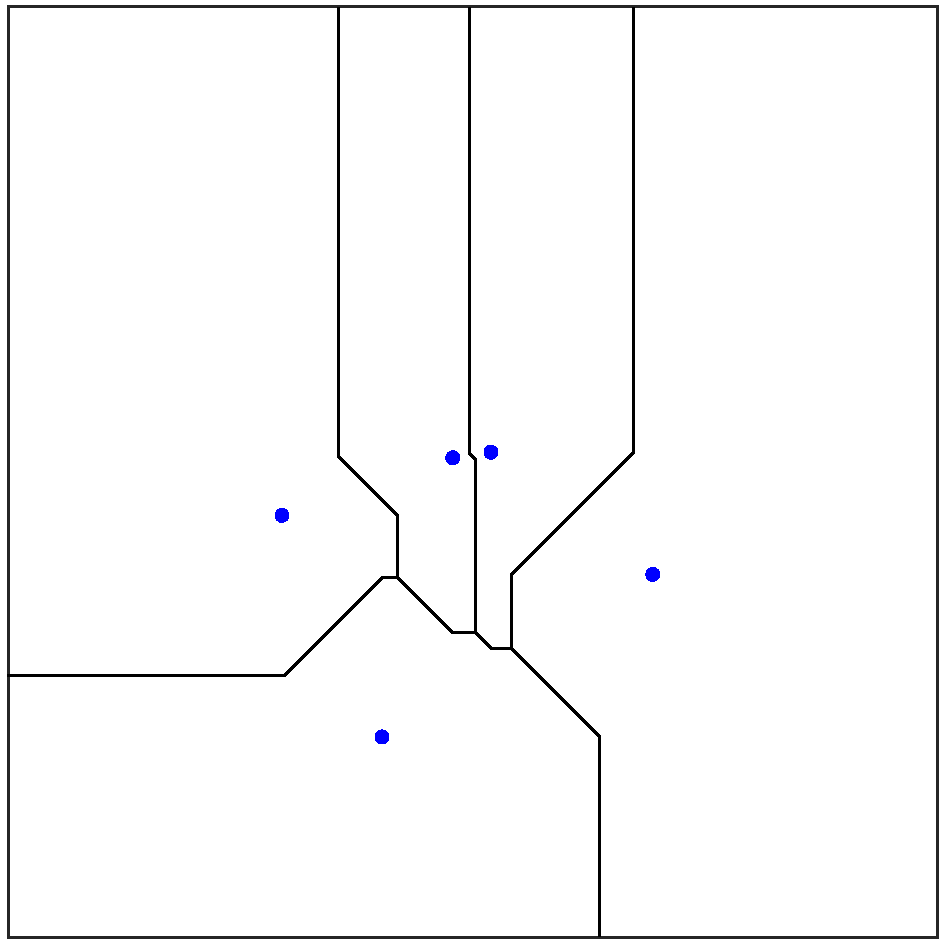
\includegraphics[width=\textwidth]{Graphics/Voronoi_manhattan.pdf}
		\caption{Voronoi diagram constructed using the Manhattan metric}
		\label{fig:manhattan}
	\end{subfigure}
	~
	\begin{subfigure}[b]{0.315\textwidth}
		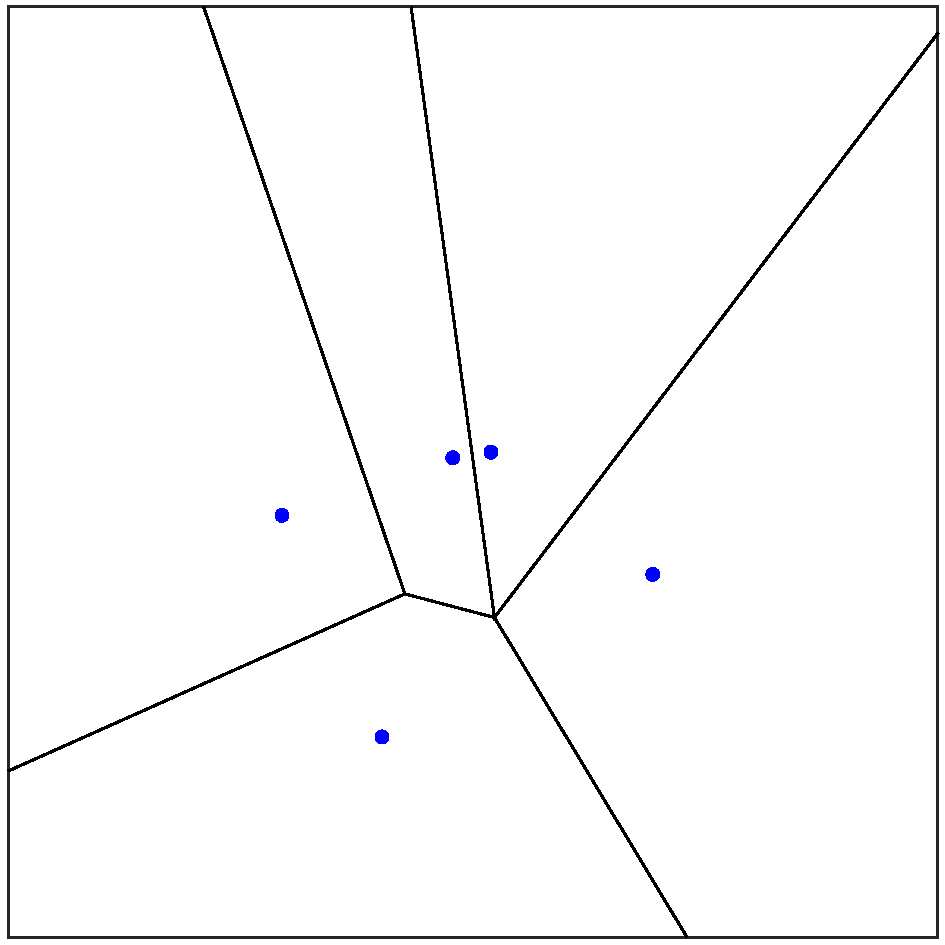
\includegraphics[width=\textwidth]{Graphics/Voronoi_euclidean.pdf}
		\caption{Voronoi diagram constructed using the Euclidean metric.}
		\label{fig:euclidean}
	\end{subfigure}
	~
	\begin{subfigure}[b]{0.315\textwidth}
		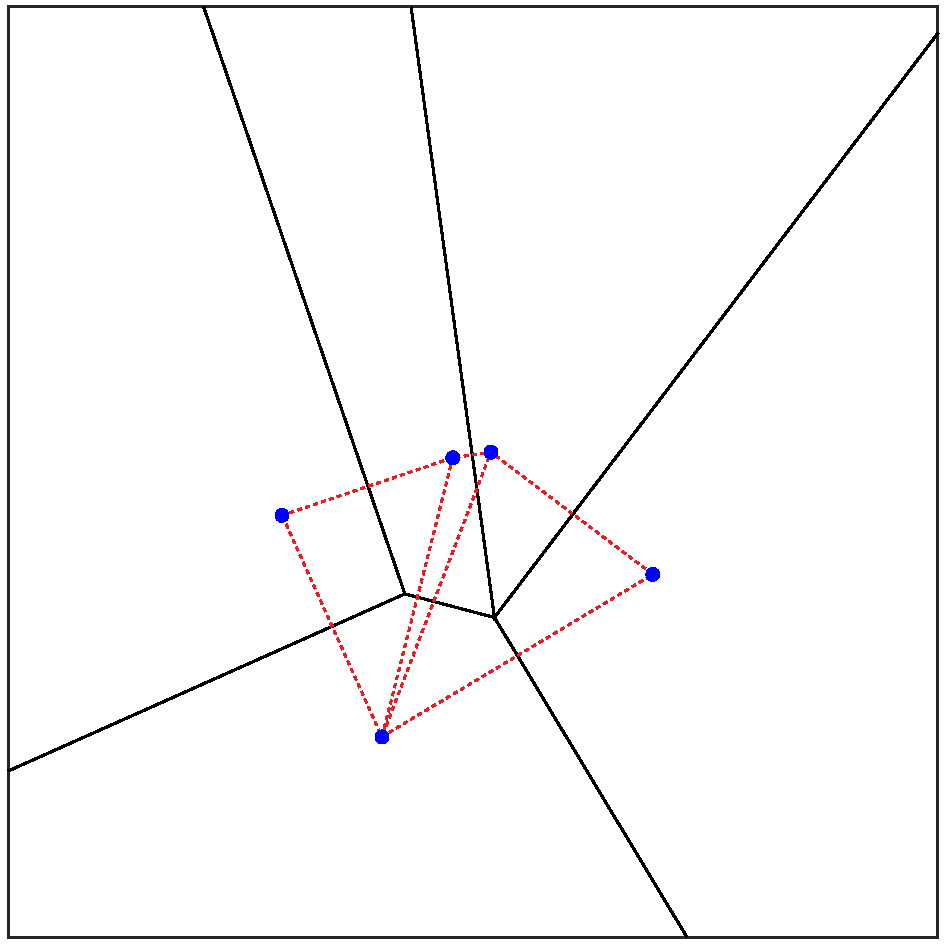
\includegraphics[width=\textwidth]{Graphics/Voronoi_Delaunay.pdf}
		\caption{Voronoi diagram and corresponding Delaunay tessellation.}
		\label{fig:delaunay}
	\end{subfigure}
	\label{fig:voronoi}
\end{figure}

The average point or average location of a Voronoi set is referred to as the \emph{centroid}. This point minimises the sum of distances to all points within the Voronoi set. When a firm locates at the \emph{centroid} of its market, it constitutes a local socially optimal location. The \emph{centroidal Voronoi tessellation} (CVT) is a special case of the Voronoi diagram where each \emph{seed} is located at the centroid of its respective set. If all firms locate at their respective \emph{centroid} it creates a \emph{centroidal Voronoi tessellation}. This is a global socially optimal solution, since it minimises the average distance between consumers and firms \citep{Laver_Sergenti_2011}. Any \emph{centroidal Voronoi tessellations} is optimal, but not necessarily unique. Given for instance 2 firms in a square space there are several CVTs; the firms could locate left-right splitting the market in half vertically, the firms could locate up-down such that they split the market in half horizontally, and so on. In each case the average distance to firms is minimised and the location of firms constitutes a social optimum. The \emph{Lloyd's algorithm} generates a \emph{centroidal Voronoi tessellation} from any generic Voronoi diagram. At every iteration, the algorithm moves the \emph{seeds} to the centroid of their current Voronoi set. Using this iterative process any Voronoi diagram converges to a \emph{centroidal Voronoi tessellation}. One of the decision rules used in this paper, is in fact an implementation of the \emph{Lloyd's algorithm}. And so when we compare the results from this baseline decision rule to the other decision rules, we are comparing with the social optimum location of firms.

The dual of the Voronoi diagram is the \emph{Delaunay tessellation} \citep[chapter~19]{Eiselt_Marianov_2011}. The \emph{Delaunay tessellation} links \emph{seeds} with adjacent Voronoi sets and the length of each of these link is the distance between the pair of \emph{seeds}, see figure~\ref{fig:delaunay}. Reformulated in terms of firms, the Delaunay tessellation is a network that links firms with a common market boundary (i.e. direct competitors). In figure~\ref{fig:delaunay} the firm located furthest left and furthest right are not linked since they do not share a market boundary. The two firms are not in direct competition with one another over any of the customers. However both firms are linked to the firm at the bottom.


The \emph{Voronoi game} originates from the study of Voronoi diagrams. This competitive location model shares features with the Hotelling model. In the Voronoi game two firms place $n$ number of facilities each and consumers shop at the nearest facility. The game is sequential so firms take turns and place one facility each turn. The game ends after $2n$ turns when both firms have placed all their facilities, and the winner is the firm with a majority of consumers. In the continuous line market the follower has a winning strategy that captures $\frac{1}{2+\epsilon}$ of the market, however the leader has a strategy that can make $\epsilon$ arbitrarily small \citep{Ahn_Cheng_Cheong_2001}. The two-dimensional Voronoi game is significantly more difficult to solve. In a one-round version of the Voronoi game -- where each firm places all its $n$ facilities in its first turn -- the follower still has a winning strategy, but the leader cannot make $\epsilon$ arbitrarily small, if consumers are distributed over a square area \citep[chapter~9]{Eiselt_Marianov_2011}. On the other hand, if consumers are distributed over a rectangular area that is sufficiently oblong, then the leader has a winning strategy \citep{Fekete_Meijer_2005}. \citet{Fekete_Meijer_2005} furthermore show that the follower's problem is NP-hard in the two-dimensional one-round game.

\subsection{Hinterlands and vertical product differentiation}

The choice of space influences results. As seen above when moving from one-dimensional to two-dimensional space it changes the equilibrium, and sometimes removes the equilibrium altogether. Similarly the shape of the space (e.g. disc, square, rectangular) and whether the space is bounded or unbounded affects the results. Certain combinations of shape and boundary creates \emph{hinterlands}, i.e. remote regions or sparsely populated regions. Competing firms will find it less attractive to locate in these regions. And as a result the papers that consider spaces without naturally occurring hinterlands -- such as the one-dimensional circular market -- find that firms locate more evenly across the entire space \citep{Eaton_Lipsey_1975, Salop_1979}.

Competitive location models are often described in terms of geographic location. However these models are also applicable when studying product differentiation, e.g. manufactures competing with one another when choosing product characteristics such as size, colour, and the shape of their respective products. When the model is formulated in terms of geographic location, then the ideal point of the consumers is his or her location. Every consumer would ideally want a firm to locate at his or her doorsteps, so the consumer avoids transportation costs altogether. In terms of product differentiation the ideal point is the consumer's preferred product characteristics. The transportation cost is replaced by the degree of disutility from consuming a product that is different from ones preferred product. The ideal points are distributed over the space, and so the consumers have heterogeneous preferences regarding products or firms. The models discussed so far strictly relate to \emph{horizontal product differentiation}. Thus even when all firms charge the same price, firms are always able to achieve positive demand, through differentiation. There are niches that guarantee the firm a positive demand. This is not the case with \emph{vertical product differentiation}, such as product quality. With \emph{vertical product differentiation} the preferences of consumers are homogenous, i.e. all consumers prefer high quality products to low quality products. If all firms charge the same price, then the firm with the highest product quality will capture the entire market. No niches exists. The two-dimensional Hotelling model assume \emph{horizontal production differentiation} along both dimensions. An alternative model is the Launhardt model \citep{Ferreira_Thisse_1996}. The model includes both \emph{horizontal} and \emph{vertical product differentiation}. It can be seen as an extension of the Hotelling model\footnote{Although the Launhardt model can be seen as an extension of the Hotelling, the paper by Launhardt was published 44 years before Hotelling published his paper.} in that firms choose location, but the firms have different delivery prices. The delivery prices is an easy way to incorporate \emph{vertical product differentiation} into the model. The delivery price is part of the \emph{transportation cost} paid by consumers. Consumers still shop at firm with the lowest total price (\emph{mill price} and \emph{transportation costs}), thus all consumers prefer low delivery prices over high delivery prices. The Launhardt model is in a sense two dimensional. The dimension along which firms locate assumes \emph{horizontal product differentiation}, while the delivery price dimension assumes \emph{vertical product differentiation}.

\subsection{Foresight}

\citet{Prescott_Visscher_1977} criticise the Hotelling model for its assumption of costless relocation. The Hotelling model implicitly assumes that firms can always relocated at a future point in time at low cost, and therefore firms, when they choose their location, do not need to take account of future entry into the market. Instead they propose a sequential location model, where it is prohibitively expensive to relocate, and where firms therefore use foresight when choosing their location once-and-for-all. Given rational expectations, firms can deduce the optimal solution by reasoning backwards from the final stage of the problem, thereby determining the sequence of optimal actions for every firm in each stage, i.e. each firm chooses the profit maximising location subject to the location of firms already in the market, and subject to the rules that future rational entrants will use. Let $N$ denote the exogenously determined number of firms in the market. The model is solved using backwards induction, i.e. the last firm entering the market will choose the location that maximises its profit given the position of all other firms already located in the market. The second last firm (firm number $N-1$) uses the position of all $N-2$ firms already located and the best response of the last entering firm when choosing its location. Firm number $N-2$ use the position of the first $N-3$ firms and the best response of firm number $N-1$ and $N$, and so forth. This continues all the way to the first firm. This process of reasoning from a set of premises, until one reaches the logical conclusion is known \emph{deductive reasoning}.

\citet[chapter~11]{Arthur_2014} is highly sceptical of this approach. Noting that there may be simple cases where every firm can figure out what to do, and where this approach produces the correct equilibrium predictions. But in more complicated scenarios or large problems with many firms the backwards induction approach is likely to break down. The approach requires sequential location and assumes \emph{common knowledge} and \emph{common knowledge of rationality}. That is each firm knows the preferences of all other firms, and each firm knows that all other firms knows the preferences of all firms, in an infinite regress. In addition each firm knows that all other firms behave rationally, and each firm knows that all other firms knows that all firms will behave rational, also in an infinite regress. To solve the model it is common to assume that firms are homogenous, both in terms of expectations and available information. Furthermore the optimal location must be unique. If any firm is uncertain about the preference or rationality of another firm, then the pure-strategy equilibrium solution breaks down. In essence when a firm has to choose its own location, the location of other firms is unknown. The firm can use the predicted location of the other firms. But the location outcome that each firm is trying to predict, depends on predictions that the firm and other firms form. \emph{``Predictions are forming a world those predictions are trying to forecast''} \citep[p.~175]{Arthur_2014}. This self-referential loop leads to logical indeterminacy, and thus without some coordination device or without assuming homogenous firms, the maximisation problem is ill defined and cannot be solved deductively. No logical conclusion exists rendering \emph{deductive reasoning} void. Nonetheless firms still make decisions even when faced with such ill defined problem. One possibility is that firms use heuristics or rules of thumb. \citet[chapter~11]{Arthur_2014} discusses these issues in terms of a competitive location model, but does not propose a new location model that incorporates or overcomes these limitations. Instead \citet[chapter~11]{Arthur_2014} looks at a model on asset pricing with many similarities, but which is easier to solve since each investors only need to predict a single outcome -- the stock price. In the location model each firm needs to predict $N-1$ outcomes, i.e. the location of all other firms. 

In the \emph{Santa Fe Artificial Stock Market} discussed by \citet[chapter~3, chapter~11]{Arthur_2014} investors are heterogeneous both in terms of information and the expectation models they use to predict the stock price. Investors hold several hypotheses on the expected stock price\footnote{More precisely, investors try and predict a linear combination of stock price and dividend. Dividend follows a stochastic autoregressive process, $AR(1)$, which is unknown to investors. And the stock price is given by the market clearing price after investors have chosen between the risky stock and a risk-free bond with a fixed rate $r$. Investors have a constant absolute risk averse utility function.}, all of which are based on the recent history of the stock price. They act on the hypothesis that suit the current state of the market and that has provided the most reliable predictions in the past. In each period, when the actual stock price is revealed, investors update the accuracy of their hypothesis. They continuously discard poorly performing hypotheses and form new hypotheses. \citet{Arthur_2014} refers to this as \emph{inductive reasoning}, i.e. deriving principles or conclusions from observation and viewing conclusions as \emph{probable}, rather than \emph{certain}. Investors act on the hypothesis viewed most probable to hold true, and update hypothesis in response to new information or observations that falsifies currently held hypothesis. In their decision process investors use \emph{inductive reasoning} as opposed to \emph{deductive reasoning}.

More specifically, the Santa Fe Artificial Stock Market model is an agent-based model, where the investors are agents. Investors hold $M$ different hypotheses, each with a corresponding linear forecasting model. Each hypothesis is a \emph{condition/forecast} rule, such that if the current state of the market matches the conditions in the hypotheses, then the hypotheses is said to be \emph{active}. Of all the active hypothesis, the investor then uses the linear forecasting model from the hypotheses that has the best accuracy. Thus investors are able to recognise patterns in state of the market, and act using their most reliable hypotheses. The state of the market is summarised by a 12-bit array. Each bit corresponds to a scenario and takes the value 0 or 1 indicating whether the scenario is true or false. They use scenarios such as the \emph{``the price has risen in the last 3 periods''} or \emph{``the current price is not larger than 16 times the dividend divided by fixed rate r''}. The combination of these 12-bits yield more than 4,000 different states of the market. 

Learning becomes a necessity once fully rational agents are replaced by agents with bounded rationality. Bounded rational agents do not act irrational, but act as best according to their knowledge and skills, and learning gives agents the potential to gradually discover optimal actions. Two types of learning exists in economics \citep[chapter~4]{Ehrentreich_2007}. With \emph{rational-based learning} agents act optimally given their available information and when new evidence arrives they update their prior opinion in a rational fashion. Bayesian learning is one example of \emph{rational-based learning} where agents hold several hypotheses. The probability of a given event occurring is conditional on the associated hypothesis. When agents observe a given event, they increase the probability of the hypothesis for which the event is most likely. In this way agents rationally update their prior opinion. The other type of learning is \emph{biologically inspired learning}. This type of learning mimics natural evolutionary selection processes, and is highly effective in terms of creating well-adapted ``species'' or strategies in an ever-changing environment. Rather than updating existing hypothesis, agents develop new hypotheses by mutating and recombining existing hypothesis. These processes are known as \emph{mutation} and \emph{crossover} respectively. Mutation creates new hypotheses based on the existing hypotheses through experimentation and unintended mistakes. While crossover creates new hypotheses by combining randomly selected bits and pieces of existing hypothesis. To increase the performance both \emph{mutation} and \emph{crossover} are often coupled with selection, such that new hypothesis are based on the best performing existing hypothesis. Genetic algorithms are used to model \emph{biologically inspired learning}. \citet[chapter~3]{Arthur_2014} uses a genetic algorithm to create new hypothesis through \emph{mutation} and \emph{crossover}.

\citet[chapter~3]{Arthur_2014} finds that the model is able to capture both the \emph{rational expectations regime} and what they call the \emph{complex regime}. In the former the model reproduces the equilibrium found analytically by assuming rational expectations and homogenous agents. That is the equilibrium where the stock price is the fundamental value, i.e. the sum of all future dividend in present value terms. There is no herd effects, technical trading remains unprofitable, and trading volume is low. The model produces the rational expectation regime when investors discover new hypotheses at a slow rate. While the model produces the \emph{complex regime} when using a faster exploration rate of new hypotheses. In the complex regime it is profitable for investors to engage in technical trading, since the herd effect produces bubbles and crashes in the stock price, and the trading volume is high. 

In this paper we incorporates \emph{inductive reasoning} into the competitive location model, using a modified version of the above described model. Section~\ref{sec:foresight} provides further details and details on the modification need to incorporate \emph{inductive reasoning} into a location model.

\subsection{Agent-based modelling}

Agent-based models are build from the bottom up, in the sense that the model consist of many autonomous and interacting agents. Each agent has strictly local motives and through the interaction of all the agents emerges the macro-behaviour of the system \citep[chapter~2]{Ehrentreich_2007}. Agents are often heterogeneous and thus the macro-behaviour is hard to predict from the local motives of agents alone. Agent-based models are typically solved on a computer by setting up the decision rules of agents and observing the system as the interaction of agents play out. Although researchers use computers to run agent-based models this is not the same as solving traditional models through numerical simulation. Instead one should view the introduction of agent-based models into economics as a response to \emph{``the inappropriateness of traditional methods''}, in particular the assumptions of representative agents and rational expectations \citep[chapter~2, p.~7]{Ehrentreich_2007}. Models assuming representative agents are incapable of generating emergent phenomena, such as the \emph{complex regime} described above where one observes herd effects and technical trading. While fully rational agents with perfect information are deprived of free choice -- the only available choice is the rational course of action. While this limits the number of possible outcomes of the model making it easier to solve, it does so at the expense of what might have been more appropriate and realistic assumptions. Both assumptions are widely used in order to solve traditional models, while neither are necessary in Agent-based models. Agent-based models are thus particularly well suited when studying problems with heterogeneous agents or bounded rationality. Furthermore agent-based models are a generalisation of equilibrium economics, as seen above with the Santa Fe Artificial Stock Market model, where standard equilibrium behaviour is a special case among a much broader set of complex behaviours. Agent-based models can provide researchers with answers to problems that would be intractable using conventional analytical techniques. However as noted by \citet[p.~viii]{Laver_Sergenti_2011} \emph{``rigorously designed and analysed computational experiments, however exhaustive, will never be substitutes for flawless and elegant classical formal proofs''}. 

\citet{Laver_Sergenti_2011} construct an agent-based model. Their model investigates the competitive location behaviour of political parties competing for voters on a two dimensional policy space. Political parties choose a policy position and the voters vote for the party whose policy is closest to the voter's ideal policy. Their model shares many similarities with the two-dimensional Hotelling model with multiple firms. However to study multiparty competition they assume that the political parties use heuristics or rules of thumb to determine their location at each iteration. They run the model for several hundred iterations. They have five types of political parties with the following decision rules. \emph{Sticker}: a party that sticks to its ideological ideal policy point, no matter what. \emph{Aggregator}: A party that constantly moves towards the centre of its current voter base. \emph{Predator}: A party that moves towards its most successful competitor, trying to replicate its success. \emph{Hunter}: A party that continues to move in the same direction, if the previous move proved fruitful, and otherwise heads in the opposite direction. \emph{Explorer}: A party that surveys several directions and then move along the most lucrative direction. The last two decision rules attempts to maximise the share of votes directly. While the other decisions rules may maximise the vote share of the political party, but this would happen indirectly. Furthermore note that none of these decision rules considers the simultaneous move of competing parties. They all implicitly assume that the other parties stick to their current policy position. Hence there is no foresight and thus the decision rules are stripped of any and all strategic considerations.

\citet{Laver_Sergenti_2011} considers a continuous and unbounded space. They obtain this space by assuming that voters' ideal policy points are drawn randomly from two bivariate normal distributions. By varying the relative size and means of the bivariate distributions they are able to analyse the location behaviour of political parties when consumers are distributed symmetric around a single peak, and when the distribution of consumers is asymmetric with two peaks. They can account for the effect of both a symmetric unimodal distribution and an asymmetric multimodal distribution of voters. To simplify their analysis they rotate the space such that the mean ideal points of the two distributions only differ along one dimension. They call this the \emph{main axis of policy disagreement} between their two subpopulations of voters.

In the baseline models they investigate, the number of political parties is exogenously given and all parties use the same decision rule. They use these baseline models to analyse the location behaviour in each of the decision rules, and to gasp the differences between decision rules. The baseline model where all parties use the \emph{aggregator}-rule is an implementation of the \emph{Lloyd's algorithm}, and thus the policy position of parties converge to the socially optimal location, where the average distance to the ideal point of all voters is minimised. In the model where all parties use the \emph{hunter}-rule -- and thus continuously try to increase their vote share -- they find that parties choose policy positions that are closer to the mean ideal point of all voters than the socially optimal positions. The \emph{hunter}-parties do not agglomerate at the peaks of the voter's ideal points, but choose a position that lies at a distance to the peaks. The party achieves short-run gains by locating close or at the peak of voters' ideal points, however the response by competing parties quickly erodes these gains, leading to the long-run policy positions that lie at a distance to the peaks. Their extended model includes entry and exit of political parties and political parties with different decision rules compete with one another for voters. The decision rule of each new political party is randomly drawn with equal probability. The entry of new political parties resembles a citizen-candidate model. Citizens or voters that feel increasingly underrepresented by the current political parties form new parties. Political parties exit when they repeatedly fall below a given threshold share of voters. They compare the competitive advantages of the decision rules by measuring the average vote share and the longevity of each decision rule. \emph{Hunter}-parties capture the largest share of voters and live longest when pitted against \emph{sticker}-parties and \emph{aggregator}-parties, and when the speed at which the \emph{hunter}-parties moves sufficiently balances the exploration of new position and exploration of its current policy position. However the \emph{hunter}-rule is not robust as both the \emph{explore}-rule and \emph{predator}-rule outperforms it, when all five decision rules are pitted against one another. 

\citet{Fowler_Laver_2008} use a similar model, but run a tournament in which decision rules submitted by other researchers are pitted against one another. Researchers knew that \citet{Fowler_Laver_2008} pre-entered the \emph{sticker}, \emph{aggregator}, \emph{hunter} and \emph{predator} rules. Furthermore they assume that elections are held every twentieth iteration. The nineteen intervening periods are considered as campaign period. Parties can freely explore different policy positions in campaign periods. And only the policy positions and votes captured in an election period influence the exit and entry decision of parties. Decision rules were prohibited from using information on the distribution of voters ideal points. The decision rules submitted fall into the following categories. \emph{Tweaks of pre-entered rules}: Decision rules based on the four pre-entered decision rules, with slight modification. \emph{Centre-seekers}: Decision rules that attempt to discover the peak or centre of voters' ideal points, and position the party at the centre. \emph{Inter-electoral explorers}: Decision rules that take advantage of the campaign period to try out different policy positions, and settling at the most prosperous of these positions. \emph{Parasites}: Decision rules that try and replicate the success of other political parties, for instance by choosing a policy position close to largest political party. \emph{Satisfiers/survivors}: Decision rules that are content with a given share of the votes, or rules that only move once their vote share approaches the threshold level.

\citet{Fowler_Laver_2008} find that \emph{centre-seeker} rules generally underperform and argue (similarly to the \emph{hunter} rule above) that the short-run gains by locating at the centre of voters' ideal points critically endangers the long-run survival of the party, because of the response from other political parties. \emph{Parasite} rules are highly disruptive to the political party that \emph{hosts} the \emph{parasite}, but rarely outperform the other rules, since they typically end up capturing half of the \emph{host's} market. The \emph{inter-electoral explorers} and \emph{satisfier/survivor} rules the party faces the above mentioned trade-off between exploration of new positions and the exploration of its current policy position. The tournament winner was a satisfying parasite rule name \emph{KQ-Strat} and submitted by Kevin Quinn. Political parties using this rule jittered slightly and randomly when above the threshold level, and when below the threshold level moved towards a randomly selected competing party that was above the threshold level. A large number of the submitted rules performed worse than the pre-entered \emph{sticker} rule, and only 7 out of the 25 submitted rules performed better than the pre-entered \emph{hunter} rule. None of the decision rules use foresight per se. They all implicitly assume that competing parties stay fixed, exempt perhaps the \emph{fool-proof} rule by Jim Adams which moves the policy of the party one-fifth the average policy shift of all competing parties. While the rationale for the rule is not included in \citet{Fowler_Laver_2008}, one could argue that parties with this rule anticipate a backlash to the policy shift of all competing firms, and thus moving one-fifth\footnote{The one-fifth move seems to have originated in a paper by \citet{Adams_Somer-Topcu_2009}. The paper is an empirical investigation of the policy response of parties to policy shifts among competing political parties. They find a statistical significant shift between 0.149 and 0.196 in response to the average policy shift of competing parties.} the average shift is a reasonable action given this expectation. However the \emph{fool-proof} rule performs worse than the \emph{sticker} rule.

\subsection*{Recap}

This literature review has gone through the different location behaviours that firms use in competitive location models without prices. In the analytical models, the simplest behaviour is firms locating without foresight (\emph{zero conjectural variation}). With the \emph{minimax strategy} firms foresee the entry of new firms (or the relocation of existing firms), in a manner that will cause maximum damage to the market of the firm. The firm therefore locates to minimise this damage. However the \emph{minimax strategy} does not consider whether or not the entry is a rational strategy for new firms, and thus it leads to an inadequate equilibrium concept. The rational expectations approach does consider this, but requires a sequential setup and quite restrictive assumptions. The agent-based model on asset pricing provides a path where these assumptions are relaxed while maintaining the simultaneous setup. Namely agents that use \emph{inductive reasoning} to make predictions and update their hypotheses in response to new information. The agent-based model from the literature on political science show how to go about analysing the two-dimensional Hotelling firm with multiple firms, and thus picks up where the analytical approach falls short of finding equilibria. In this agent-based model many decision rules that rely on rules of thumb have been constructed and battle tested in tournaments. However no one has so far considered decision rules with foresight. This paper will build upon this model by \citet{Laver_Sergenti_2011} but introduce agents that use \emph{inductive reasoning} as a way to reintroduce foresight into the competitive location model. The literature review has also repeatedly highlighted the difficulties in optimal solutions to location models, even those without any competitive aspects.


\section{Model}

To analyse the location behaviour of firms we construct an agent-based model\footnote{All models in this paper have been programmed from the button up. The code is available at \url{https://github.com/jsekamane/Positioning/tree/master/Models/ABM}. All the models are build in MATLAB (R2015a) and run on a MacBook Pro with a 2.6 GHz quad-core Intel Core i7 processor. In addition several of the models use MATLAB's Parallel Computing Toolbox with 4 local workers taking advantage of the quad-core processor structure to process several runs in parallel.} akin to \citet{Laver_Sergenti_2011}. We reformulate the model in terms of firms competing for customers, when they choose their geographic location. It is simply shorter to write `firms' and `relocate' rather than `political parties' and `shift policy position' and it reads more naturally. The results of the model are still valid in a political context, as well as in the context where manufacturers competing for customers through product differentiation when choosing product characteristic along two dimensions. 

The decision rule of firms is exogenously determined. In each iteration the decision rule of the firm determines its location. All firms choose their location simultaneously. The model executes several iteration and analyses how the interaction of the firms affect the overall location of firms. The model assumes that all firms charge the same price, and thus this paper abstracts away price competition, and only considers location differentiation. Price competition greatly increases the complexity of the model, and is therefore beyond the scope of this paper. Furthermore firms can and do change prices more frequently than they change location. Thus price competition and location competition take place on two different time scales -- a fast and a slow. It remains an open question how to appropriately incorporate the different time scales into an unified iterative model.

\subsection{Consumers}

The scope of this paper is limited to one side of the market -- the firms and their decision-making behaviour. For this reason simplifying assumptions are used for the other side of the market -- the consumers and the purchasing behaviour of consumers. For one thing consumers are static. They do not shift position, they maintain preferences, they are obliques to trends, and are in no way influenced by changes in the market. Secondly consumers behave non-strategically and demand inelastically. They always purchase a single unit from the closest firm, regardless of the distance to the firm. And finally all firms are identical in the eyes of the consumer. There is no brand recognition and no loyalty -- the customer purchase from the closest firm regardless of previous purchasing history.

Every consumer has an ideal point in the market. This is the point where the consumer wants a firm to locate. All other points are second to the ideal point. And the further away from the ideal point that the firm locates, the less attractive it becomes. Consumers have \emph{single peaked preferences}. Essentially this paper reduces consumers to being merely their ideal points. 

Viewed in terms of geography the ideal point would be the consumer's physical location and the distance is the bee-line distance to firms. Alternatively the model can be viewed in terms of product differentiation. Then the ideal point of the consumer is his or her desired product characteristic along the two dimensions. We assume \emph{horizontal product differentiation} along both dimension, i.e. product characteristic are non-ordinal. In addition we need to assume that product characteristics are continuous and infinitely divisible.

The utility function for each consumer is a function of the distance from the consumer's ideal point and to the position of the firm. The utility function is equivalent to a quadratic loss function. The Euclidean distance metric is used. The utility of customer $i$ is the negative squared distance between customer $i$ and the closest firm $j$:

\begin{equation}
	U_i(j) = -d(i,j)^2
	\label{eq:utility}
\end{equation}

\subsubsection{Consumer distribution}

The simplification of consumer's behaviour allows focused attention on the behaviour of firms. As discussed in the literature review the distribution of consumers can fundamentally change the behaviour of firms. We would like to capture and analyse these changes -- in particular the effects from asymmetric and multimodal distributions. We follow the method used by \citet{Laver_Sergenti_2011} and assume two consumer subpopulations in our market. When the two subpopulations have the same mean ideal point then the aggregated distribution of consumers will be symmetric and unimodal. While subpopulations with vastly different mean ideal points and different sizes will lead to an aggregated distribution of consumers that is asymmetric and bimodal. Thus this method of using two subpopulations is able to capture several different types of aggregate distributions using only two parameters; the polarisation of subpopulation ideal points, and the relative size of the two subpopulations. 

The market is two-dimensional, so we use the two-dimensional equivalent of the \emph{normal distribution} -- the \emph{bivariate normal distribution}. Both subpopulations follow a bivariate normal distribution. Using different mean values in the distribution imply that the subpopulations disagree over the ideal point. Without further restrictions the subpopulations would disagree on both dimensions. To simplify the analysis, and without lose of generality, we assume that the subpopulations have a common ideal point along one dimension and only disagree over the ideal point along the other dimension. This is equivalent to rotating the market space or coordinate system until disagreement only appears along one of the dimensions, i.e. rotating the market space such that the line going through the mean ideal points of subpopulations is parallel to an axis. One can always rotate the coordinate system without loss of information, and so this simplifies our analysis without any loss of generality. This is similar to the orthogonal transformation underlying a \emph{principal component analysis}. We start out with two dimensions (or two components), and end up with two new dimensions (two principle components); the disagreement dimension (x-axis) and the agreement dimension (y-axis). The two subpopulations -- from now on referred to as `left' and `right' -- follow a \emph{bivariate normal distribution} with mean $(-\mu,0)$ and $(\mu,0)$ respectively, and both with standard deviation $(0.5, 0.5)$\footnote{That is, $(\mu_{x,l},\mu_{y,l}) = (-\mu,0)$ and $(\mu_{x,r},\mu_{y,r}) = (\mu,0)$, while the standard deviation is $(\sigma_{x,i},\sigma_{y,i}) = (0.5, 0.5)$ for $i = \{l,r\}$. We further assume no correlation among the two dimensions. The correlation coefficient $\rho$ is zero and thus the covariance matrix is $\left[ {\begin{array}{*{20}{c}} {{{0.5}^2}}&0\\ 0&{{{0.5}^2}} \end{array}} \right]$.}. Where the parameter $\mu$ measures the ideal point polarisation. The parameter measuring the relative size of the left subpopulation is $n_l/n_r$. The aggregated consumer distribution is a \emph{mixed bivariate normal distribution} with weights based on the relative size of the subpopulations \citep{Weisstein_2002b, Balakrishnan_Lai_2009}:

\begin{equation}
f(x,y) = \frac{n_l/n_r}{1+n_l/n_r} f^{(l)}(x,y) + \frac{1}{1+n_l/n_r} f^{(r)}(x,y), \quad f^{(i)}(x,y) = \frac{e^{-\frac{(x-\mu_{x,i})^2}{2(\sigma_{x,i})^2} - \frac{(y-\mu_{y,i})^2}{2(\sigma_{y,i})^2}}}{2\pi\sigma_{x,i}\sigma_{y,i}}
\end{equation}

The mean ideal point on the y-axis is 0 for both subpopulations hence no disagreement along this dimension. The mean ideal point on the x-axis is $-\mu$ for the left subpopulation and $\mu$ for the right subpopulation. For $\mu > 0$ there is disagreement along the x-axis. I will analysis the polarisation parameter in the range $\mu \in [0, 1.5]$ -- a range that spans both an unified and a split market. At the lower bound of the range there is no disagreement and the market consists of one unified customer base. At the upper bound there is essentially no overlap between the subpopulations and the customer base is split. The range of the relative subpopulation size is $n_l/n_r \in [1, 2]$. The subpopulations are equally large when the $n_l/n_r = 1$, while $n_l/n_r = 2$ indicates that the left subpopulation is twice the size of the right subpopulation. See figure~\ref{fig:distribution}.

The default unit of measure throughout this paper will be standard deviations. This unit of measure will refer to the standard deviation measurement used in the bivariate normal distributions, e.g. when this paper reports that the distance between two points is 1 standard deviation, then this is equivalent to twice the standard deviation in the subpopulation distribution. The unit of measure is independent of the space and the coordinate system, making it easier to compare results with other studies.

\begin{figure}[htp!]
	\caption{Example of market where the left subpopulation is twice as large as the right ($n_l/n_r = 2$) and the polarisation of the mean ideal points is respectively $\mu = 0.5$ (left) and $\mu = 1.5$ (right).}
	\centering
	\begin{subfigure}[t]{0.485\textwidth}
		\includegraphics[width=\textwidth, trim={15mm 90mm 20mm 70mm}]{Graphics/distribution_mu05_nratio2.pdf}
		\caption{}
		\label{fig:surface_mu05}
	\end{subfigure}
	~
	\begin{subfigure}[t]{0.485\textwidth}
		\includegraphics[width=\textwidth, trim={15mm 90mm 20mm 70mm}]{Graphics/distribution_mu15_nratio2.pdf}
		\caption{}
		\label{fig:surface_mu15}
	\end{subfigure}
	\caption*{(a), (b) Distribution of consumer ideal points.}
	
	\begin{subfigure}[t]{0.485\textwidth}
		\includegraphics[width=\textwidth, trim={15mm 85mm 20mm 75mm}]{Graphics/contour_mu05_nratio2.pdf}
		\caption{}
		\label{fig:contour_mu05}
	\end{subfigure}
	~
	\begin{subfigure}[t]{0.485\textwidth}
		\includegraphics[width=\textwidth, trim={15mm 85mm 20mm 75mm}]{Graphics/contour_mu15_nratio2.pdf}
		\caption{}
		\label{fig:contour_mu15}
	\end{subfigure}
	\caption*{(c), (d) The contours of the distribution. The dots are an example of how five firms might locate.}
	
	\begin{subfigure}[t]{0.485\textwidth}
		\includegraphics[width=\textwidth, trim={15mm 80mm 20mm 75mm}]{Graphics/marketarea_mu05_nratio2.pdf}
		\caption{}
		\label{fig:marketarea_mu05}
	\end{subfigure}
	~
	\begin{subfigure}[t]{0.485\textwidth}
		\includegraphics[width=\textwidth, trim={15mm 80mm 20mm 75mm}]{Graphics/marketarea_mu15_nratio2.pdf}
		\caption{}
		\label{fig:marketarea_mu15}
	\end{subfigure}
	\caption*{(e), (f) The market area of each of the five firms. The dots are the location of the firm. The crosses are the market centroids (weighted with the probability mass within each respective market).}
	
	\label{fig:distribution}
\end{figure}

Given the aggregated consumer distribution one approach would be to randomly draw a finite number of consumers from the distribution. Market shares can then be calculated by counting the number of consumers. This paper, like \citet{Laver_Sergenti_2011}, will not employ this approach. Instead the consumer distribution is carried through and market shares are calculated by aggregating probability mass. Similarly the centroid of the market is weighted by the probability mass rather than the number of consumers (centroid shown in figure~\ref{fig:marketarea_mu05} and~\ref{fig:marketarea_mu15}). Although the two approaches yield the same results on average, the latter is independent of particular draws, thus we save computational power not having to execute several repetitions to obtain average values.

We will now evaluate the consumer distribution function, with particular focus on the combinations of the parameter values that give rise to a single peak in the distribution, and the combinations which give two peaks. This information will help us interpret the results of the model later on. The consumer distribution function is a mixed bivariate normal distribution. The distribution is symmetric along the y-axis, so the peaks and saddle points of the distribution will all have coordinate zero, $y^p = y^p_r = y^p_l = y^s =0$. We need only focus on determining the coordinates of the peaks and saddle points along the x-axis. Because of the symmetry along the y-axis and since there is no covariance between x and y in the bivariate normal distributions, we can determine the x-coordinates using the marginal probability function $f_x$. This function is equivalent to a mixed univariate normal distribution \citep{Weisstein_2002a, Weisstein_2002b, Balakrishnan_Lai_2009}. We express the function in terms of the free parameters; polarisation of the ideal points of the subpopulation, $\mu$, and the relative size of the subpopulation $n_l/n_r$:

\[
f_x(x,\mu,n_l/n_r) = \frac{n_l/n_r}{1+n_l/n_r} \frac{ e^{-\frac{(x+\mu)^2}{2\left(\frac{1}{2}\right)^2}}}{\sqrt{2\pi}\sqrt{\frac{1}{2}}} + \frac{1}{1+n_l/n_r} \frac{ e^{-\frac{(x-\mu)^2}{2\left(\frac{1}{2}\right)^2}}}{\sqrt{2\pi}\sqrt{\frac{1}{2}}}
\]

To find the extrema of the function we differentiate with respect to $x$:

\[
\frac{\partial f_x(x,\mu,n_l/n_r)}{{\partial x}} = \frac{n_l/n_r}{1+n_l/n_r} \frac{ e^{-2(x+\mu)}}{\sqrt{\pi}}\left(-4(x+\mu)\right) + \frac{1}{1+n_l/n_r} \frac{ e^{-2(x-\mu)}}{\sqrt{\pi}}\left(-4(x-\mu)\right)
\]
\[
= \frac{-4e^{-2(x+\mu)} \left((x+\mu)n_l/n_r + (x-\mu)e^{8x\mu} \right) }{(1+n_l/n_r)\sqrt{\pi}}
\]

Setting the derivative equal to zero and rearranging gives:

\[
\frac{\partial f_x(x,\mu,n_l/n_r)}{{\partial x}} = 0 \Leftrightarrow (x+\mu)n_l/n_r + (x-\mu)e^{8x\mu} = 0
\]
\begin{equation}
\Leftrightarrow n_l/n_r = - \frac{x-\mu}{x+\mu} e^{8x\mu}
\label{eq:extrema}
\end{equation}

It is not possible to solve for x, so instead we plot the equation in a $(\mu, x)$ diagram to evaluate the expression, see figure~\ref{fig:bifurcation}. The curve splits into several branches revealing the bifurcation, i.e. for specific combinations of $\mu$ and $n_l/n_r$ our x takes on multiple values \citep{Strogatz_1994}. As $\mu \to 0$ implies $x \to 0^-$ when approaching from the negative side. However as $\mu \to 0$ and $x > 0$ we will observe a jump between $\mu \simeq 0.657$ and $\mu = \frac{1}{2}$. The bifurcation implies that all the models in this paper are non-linear.

\begin{figure}[ht!]
	\centering
	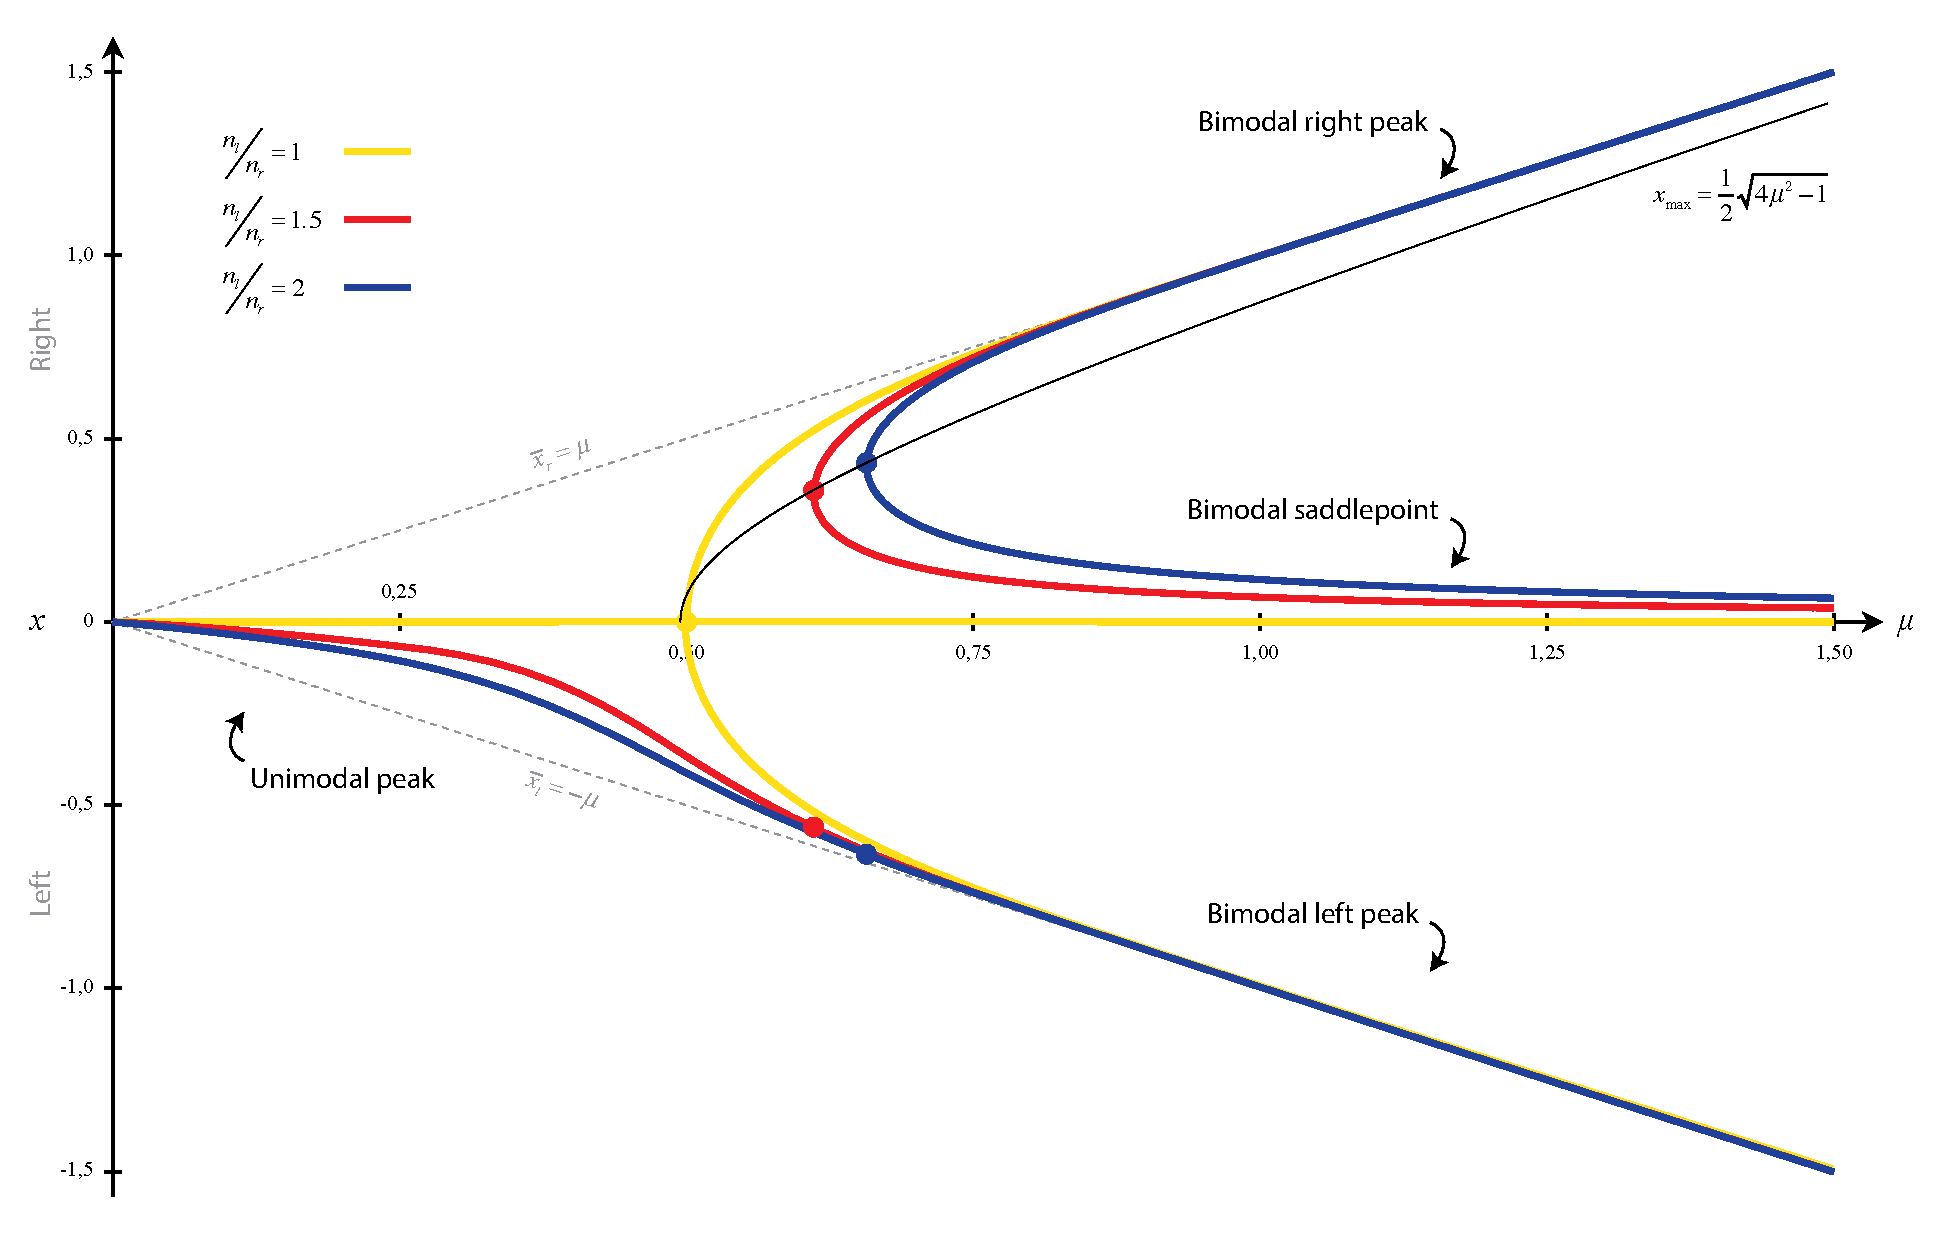
\includegraphics[width=\textwidth]{Graphics/Bifurcation.pdf}
	\caption{Bifurcation diagram. The curves indicate the extrema of the population density function along the x-axis. The left subpopulation is respectively twice as large (yellow curve), half as large (red curve) and just as large (blue curve) as the right subpopulation. The grey dotted lines indicates the mean ideal points of each subpopulation. The solid black line separates the right peak of the distribution from the saddle point at different relative sizes of the subpopulations. The dots indicate the breaking point between the unimodal distribution and the bimodal distribution.}
	\label{fig:bifurcation}
\end{figure}

Unsurprisingly we see that with no polarisation, $\mu = 0$, the distribution is unimodal with a single peak at $x^p=0$ regardless of the relative size of the subpopulation $\left(\forall n_l/n_r\right)$. With a low degree of polarisation, $\mu \in \left]0,\frac{1}{2}\right]$, the distribution remains unimodal with a unique peak in between the origin and the mean ideal point of the left-subpopulation, $x^p \in \left]0,{\bar x_l}\right[$, where the mean ideal point is ${\bar x_l} = -\mu$. The relative size of the subpopulation determines the exact value of $\mu$, for which the distribution becomes bimodal. With subpopulations of equal size, $n_l/n_r=1$, the distribution is bimodal for $\mu > \frac{1}{2}$. In addition the peaks of the distribution are located at equal distance to the origin, while the saddle point is located at the origin, $x^s = 0$. As the relative size of the subpopulation increases so does the value of $\mu$, for which the distribution becomes bimodal. To determine this breaking point, we can differentiate equation~\ref{eq:extrema} with respect to $x$\footnote{$\frac{\partial n_l/n_r}{{\partial x}} = - \frac{2 \mu e^{8x\mu} \left(4\mu^2-4x^2-1\right)}{(\mu+x)^2} = 0$ $\Leftrightarrow x_{max} = \frac{1}{2} \sqrt{4{\mu}^2-1} \Leftrightarrow \mu_{max} = \frac{1}{2} \sqrt{4x^2+1}$ where $x_{max}$ (or $\mu_{max}$) is the breaking point between the right peak and the saddle point of the distribution. By substituting $x_{max}$ into equation~\ref{eq:extrema} we get an expression for the breaking point in terms of the combinations of $\mu$ and $n_l/n_r$: $n_l/n_r = - \frac{\sqrt{4{\mu}^2-1} -2\mu}{\sqrt{4{\mu}^2-1} +2\mu} e^{4\sqrt{4{\mu}^2-1}\mu}$. Further note that if $n_l/n_r$ is lower than the right-hand side of the equation, then the distribution is bimodal, and visa versa. At the upper limit of our range, when the left subpopulation is twice as large as the right ($n_l/n_r=2$), we have that $\mu \simeq 0.657$, i.e. for any $\mu > 0.657$ the distribution is bimodal.}. As the polarisation of the subpopulation, $\mu$, increases the peaks of the distribution converges towards the mean ideal points of each subpopulation, $x^p_r \to {\bar x_r} = \mu$ and $x^p_l \to {\bar x_l} = -\mu$. With an unequal sized subpopulations, $n_l/n_r > 1$, the saddle point lies slightly to the right of the origin, $x^s > 0$. The asymmetric bifurcation diagram arises, because we choose to model the left subpopulation larger than the right, by choosing the range $n_l/n_r \in [1,2]$.

%Table~\ref{tab:distribution} provide descriptive statistics on the consumer distribution and the coordinates for the peaks of the distribution.
%\begin{table}[h!]
%	\caption{Summary of consumer distribution. \TODO }
%	\begin{tabular}{ p{0.145\textwidth} p{0.145\textwidth} | p{0.145\textwidth} p{0.145\textwidth} | p{0.145\textwidth} p{0.145\textwidth}}
%		\multicolumn{2}{l}{\emph{Parameters}}					& \multicolumn{2}{c}{\emph{Agg. distribution}} 	& \multicolumn{2}{c}{\emph{Coordinates of peaks}}  \\
%		Relative size					& Polarisation			& Mean ideal point 		& Standard deviation		& Left peak	 					& Right peak \\
%		$n_l/n_r$						& $\mu$					& ${\bar \mu}_{x,pop}$	& $\sigma_{x,pop}$			& $x^p_l$ (or $x^p$)			& $x^p_r$ \\
%		\hline
%		1 								& 0.5            		& 0.000        			& 0.707         			& -0.070					 	& - \\
%		1        						& 1.0            		& 0.000            		& 1.118           			& -0.995					 	& 1.001 \\
%		1        						& 1.5            		& 0.000            		& 1.581          			& -1.479					 	& 1.497 \\
%		2        						& 0.5            		& -0.167	    		& 0.687         			& -0.404					 	& - \\
%		2        						& 1.0            		& -0.333	      		& 1.067          			& -0.997					 	& 0.996 \\
%		2        						& 1.5            		& -0.500        		& 1.500            			& -1.495					 	& 1.495 \\
%		\hline
%	\end{tabular}
%	\label{tab:distribution}
%	\Fignote{the coordinates of the peaks of the distribution are solved numerically.}
%\end{table}

\subsection{Firm behaviour}

We now turn our attention to the behaviour of firms. Below we present the decision rules, the underlying rationale for each rule, and the assumptions and information necessary for each rule. We only present the decision rules without foresight here. Once we have analysed the model with these rules and gotten a better understanding of each rule, we will extend the model to include foresight and \emph{inductive reasoning}. All firms choose their location simultaneously, and in each iteration the decision rule of the firm determines the location of the firm.

Ideally we would want each firm to choose the location that maximises its share of the market, given the location of the other firms. However all firms choose their location simultaneously, and thus when a firm has to choose its own location, the location of other firms is unknown. The firm can use the predicted location of the other firms. But the location outcome that each firm is trying to predict, depends on predictions that the firm and other firms form. This self-referential loop leads to logical indeterminacy and so the maximisation problem is ill defined. Instead of solving the maximisation problem for the optimal location, firms may use heuristics or rules of thumb, when they choose location. The literature review provided an overview of the many different decision rules previously considered. This paper will use three of the heuristic decision rules laid out by \citet{Laver_Sergenti_2011} as the base to which other decision rules are compared. We use the \emph{sticker}, \emph{aggregator} and \emph{hunter}-rule since they represent respectively no exploration of the space, the social optimal locations, and a unceasing exploration for better locations.

\subsubsection{Sticker-rule}

The simplest decision rule a firm can use is the \emph{sticker}-rule. With this decision rule the firm sticks to its initial position regardless of what happens. This could be a firm that is either unwilling to change or incapable of change. The management of the firm may have an unyielding belief in the long-run superiority of the position of the firm, discouraging it from any change, even in times of despair, i.e. a belief that the market share of the firm will always recover and excel, in and of itself. The firm might also be unable to change, due to financially constraint such as the fixed cost of relocating or investments that cannot be recuperated. And finally, given the task of predicting the future location of all other firms, the firm might see its current position as less risky than a new location based on uncertain predictions.

\subsubsection{Aggregator-rule}

Firms using the \emph{aggregator}-rule constantly seeks to please its own customer base. The firm does not try and predict the future. Instead it takes its current market area and locates at the centre of it. More specifically the centre or \emph{centroid} is the mean ideal point of all customers of the firm. The centroid position takes into account the population density within the market area, drawing the firm towards the centre of mass (see figure~\ref{fig:distribution}).

The future location of competing firms may change and thus change the market area of the firm. And so there is no guarantee that the centroid of the current market area is identical to the centroid of the subsequent market area. Nonetheless firms using the \emph{aggregator}-rule continually pursue the mean ideal point of their customer base. Likewise there is no guarantee that the relocation of the firm will increase its share of the market, or even maintain the current share. Market shares are in a sense a secondary priority for the firm using the \emph{aggregator}-rule. The management of the firm may reason that they can retain and recruit new customers by pleasing their current customers\footnote{Noted that customer loyalty is not incorporated in the models. Customers always choose the closest firm regardless of previous purchasing history. And this might understate the efficiency of firms using the \emph{aggregator}-rule in markets with high degree of customer loyalty.}.

When all firms in the market use the \emph{aggregator}-rule then the model is an implementation of the \emph{Lloyd's algorithm} and the location of firms will converge to the stable \emph{Centroidal Voronoi Tessellation} \citep[chapter~3, pp.~48-49]{Laver_Sergenti_2011}. The \emph{Centroidal Voronoi Tessellation} (CVT) is a special geometric construction where each firm is located at the centroid of its own market area. \emph{Aggregator} firms located at the current centroid will not relocate. Hence when all firms use the \emph{aggregator}-rule the CVT is stable -- no firm relocates. The CVT has the useful property that the distance between all customers and their closest firm is minimised. The location of firms is socially optimal when the average distance to consumers is minimised. This will prove useful later on when comparing the social welfare of the different decision rules. The all-aggregator model will maximise our measure of social welfare.

The underlying requirement for an \emph{aggregator} firm is that it has perfect knowledge of its current customer base. The firm knows the span of its current market area and the distribution of customers within the area, such that the firm can correctly determine the mean ideal point of its customers.

The \emph{aggregator} firm never relocates outside its current market area. But otherwise there is no limit as to how far an \emph{aggregator} firm can move at each iteration. The firm nonetheless tends to move in relatively small steps, unless the market is extremely unstable. 

\subsubsection{Hunter-rule}

The \emph{hunter}-rule is a trial-and-error type of decision rule. The firm continues in the same direction, if it previously proved fruitful, and otherwise the firm heads in the opposite direction. At each iterations the firms move what corresponds to 0.1 standard deviation of the population distribution. If the previous move did not increase the market share, then the firm turns around and heads in a random direction drawn from the 180 degree arc now in front of it. 

Firms using the \emph{hunter}-rule never settle down. The firm endlessly hunts higher market shares with the same speed and intensity. For a firm with this decision rule there is no comfortable threshold share of the market that suffice or slows exploration. In the trade-off between exploration and exploitation the firm always chooses the first option. 

The only information used in the decision process of a \emph{hunter}-firm is the current relative change to its market share and its current direction. No information going further into the passed is used. The firm may lack memory, or may emphasis the present to such a degree that information going further back is seen as worthless. The behaviour of a \emph{hunter}-firm is most suited for a fast evolving market with high unpredictability.

The \emph{hunter}-firm moves 0.1 standard deviation each iteration. This is the \emph{speed of adaption}. It is beyond the scope of this paper to investigate the effects of changing the speed parameter. However \citet[chapter~7, pp.~150-151]{Laver_Sergenti_2011} find evidence that a speed parameter of 0.1 standard deviation is optimal for a \emph{hunter}-firm. They argue that this speed strikes the balance between quickly reaching better locations without overshooting these location when moving around. 

\subsubsection{Deliberate reaction to competitors}

The above described heuristic decision rules are good first approximation on how firms might choose to locate. Especially in a simultaneous multi-agent location model where the future location of other firms is unknown. Later on we would like to investigate how foresights affects our results. But before doing so, we need to return to the deliberate process of maximising market share, i.e. before we can answer how the firm locates given the \emph{predicted} locations of competing firms, we need a new decision rule that determines how the firm locates given \emph{any} location of competing firms. None of the above mentioned decision rule take the location of competing firms into consideration. In this section we develop a decision rule that assumes that competing firms stay at their current location. Later on we extend the decision rule so it includes location predictions and learning. In the end we will have reintroduced strategic considerations into the simultaneous location model.

For now assume that competing firms stay at their current location. We want to know where the firm should relocate to maximise its market share. When a firm relocates it gains new customers and loses others. Thus there is a trade-off between the areas of the market that it gains and the areas that it loses. To simplify matters even further we only focus on the first effect. The problem is then equivalent to a new firm entering a market -- populated with competing firms -- and choosing the location that will maximise its share. There is extensive research on competitive location models such as the Hoteling model and the Voronoi game, and on the geometry behind Voronoi diagrams. Yet only four papers provide methods on how to find the location that maximises the market of a firm in two-dimensional space. The methods all concern the location of newly entering firms. None consider the optimal location of an existing firm that relocates. \citet{Cabello_Diaz-Banez_Langerman_Seara_Ventura_2010} use the \emph{reverse nearest neighbour} method to find the position that maximises the number associated points or customers. However their method requires a finite number of points. Thus this method is not applicable, since we assume an infinitely continuous number of consumers by using the distribution of consumers. The remaining three papers use continuous distributions, but they assume the distribution is uniform, which also make them unsuited for our needs, since we have a mixed bivariate normal distribution. \citet{Averbakh_Berman_Kalcsics_Krass_2015} use a method that partitions the solution space into smaller regions. The partition is done in such a way that the structure of the Voronoi diagram is unaffected by how the firm locates within each region. The structure is only affected by which of the regions the firm locates in. The partition simplifies the problem to a \emph{search problem} over all regions. Their method uses the \emph{Manhattan} distance metric. The partitioning also work with \emph{Euclidian} distance metric. However it might be impossible to obtain exact solutions with this distance metric, because of the complexity that the \emph{Euclidian} norm introduces in the object function \citep[pp.~409-410]{Averbakh_Berman_Kalcsics_Krass_2015}. The models in this paper uses the \emph{Euclidian} distance metric. \citet{Cheong_Efrat_Har-Peled_2007} note the difficulties in finding analytical solutions to the problem and develop an algorithm that approximates the maximum of the object function. Their method finds the largest circle that is contained within each existing market area and that does not contain any of the existing firms. They construct squares with lengths equal to the radius of the largest empty circles and with the same centre as the circles. These squares are partitioned into grids and they use an \emph{$\epsilon$-approximation} method to pick the cell in the grid that maximises the market area. As previously mentioned \citet{Cheong_Efrat_Har-Peled_2007} assume a uniform distribution of customers. When working with non-uniform distributions the largest empty circles is a poor criteria to narrow down the search for maximum, since there is no guarantee that a dominant part of the density mass falls within the circle. The last paper by \citet{Dehne_Klein_Seidel_2002} proves that if the location of neighbouring firms span a convex hull, then there exists a unique local maximum inside this convex hull. They use a Newton method to calculate these local maxima within each of the Delaunay circles (that is the smallest circles covering the triangles in the Delaunay Triangulation). In addition they check for corner solutions, i.e. locating on top of existing firms. The optimal location for the new firm is then the maximum of all these local maxima. The case where the neighbouring firms do not span a convex hull is left open. And so they only provide a partial solution to the problem. There is nothing that prevent neighbouring firms from locating such that they do not span a convex hull in the models of this paper, and thus this method is not suitable either. 

None of the currently existing methods are applicable to the models used in this paper. This is due to the non-uniform infinitely continuously distribution of consumers, where neighbouring firms may not form convex hulls, and because we use the Euclidian distance metric. Since there does not exist any methods capable of finding the optimal solution, we are forced to develop a method that roughly approximates the solution. I draw on the commonalities of these papers when constructing the decision rule that explicitly tries to find the location that maximises the market share of the firm.

\subsubsection{Maxcov-rule}

Firms using the \emph{maxcov} decision rule aims for the location that maximises the number of customers. The firm assumes that the ideal location lies in the gaps between competing firms. The firm considers all the gaps and picks the one with the most consumers. Each gap is a triangle in the Delaunay Triangulation. The Delaunay Triangulation is constructed using only the location of competing firms, and the boundary points of the space, see figure~\ref{fig:maxcov}. The latter insures that the firm also considers locations that lie outside the area spanned by competing firms \citep[p.~556]{Cheong_Efrat_Har-Peled_2007}. The triangle with most consumers is selected\footnote{The triangle with the most consumers is a proxy for the actual market share obtained by the firm once it locates within the triangle. The triangle and the actual market or Voronoi set (obtained once the firm locates) differs in shape and size. The triangle with most consumers may not always be the triangle that results in the highest market share for the firm. However in 40-90\% of the cases the triangle with most consumers is also the triangle that results in the highest market share. If the firm did not locate in the triangle with most consumers, but select any one of the Delaunay triangles with equal probability, it would pick the triangle that results in the highest market share in only 4-16\% of all cases. Although this approach is not perfect, it is sufficient and computationally fast. The problem is reduced to a \emph{search problem} over all the $2+2(N-1)$ Delaunay triangles, where $N-1$ is the number of competing firms.}. The ideal location is the weighted mean ideal point of all customers within that triangle. We use the density of consumers as weights.

\begin{figure}
	\caption{Example with five competing firms (blue markers) in market where $\mu=0$ and $n_l/n_r = 1$.}
	\centering
	\begin{subfigure}[t]{0.31\textwidth}
		\includegraphics[width=\textwidth, trim={34mm 76mm 28mm 76mm}]{Graphics/maxcov_a_voronoi.pdf}
		\caption{The Voronoi diagram illustrating the market areas of competing firms.}
		\label{fig:maxcov_voronoi}
	\end{subfigure}
	~
	\begin{subfigure}[t]{0.31\textwidth}
		\includegraphics[width=\textwidth, trim={34mm 76mm 28mm 76mm}]{Graphics/maxcov_b_delaunay.pdf}
		\caption{The Delaunay Triangulation of competing firms and the boundary points. Red marker is the weighted centroid of the triangle with the largest share of customers. It indicates the ideal position of the firm.}
		\label{fig:maxcov_delaunay}
	\end{subfigure}
	~
	\begin{subfigure}[t]{0.31\textwidth}
		\includegraphics[width=\textwidth, trim={34mm 76mm 28mm 76mm}]{Graphics/maxcov_c_voronoi.pdf}
		\caption{The Voronoi diagram once we include the ideal position of the firm (red dot).}
		\label{fig:maxcov_voronoi_incr}
	\end{subfigure}
	\label{fig:maxcov}
\end{figure}

Rather than move directly to the ideal position, the \emph{maxcov}-firm, moves 0.1 standard deviations in the direction of the ideal position. There are two reasons for this gradual adjustment. First, it makes the speed at which the \emph{maxcov}-firm moves comparable to the speed of the other decision rules. Recall that the \emph{hunter}-firm moves 0.1 standard deviations, and that the \emph{aggregator} never moves outside its current market area. Secondly, the ideal position of the firm is sensitive to changes in the position of competing firms. Even minor changes may alter which of the triangles contain the most customers, and thus lead to significantly different ideal position. The gradual adjustments insures less volatile variation in the relocation pattern of the firm, which is necessary later on when other firms attempt to predict the future location of the firm.

When a \emph{maxcov}-firm chooses its location it explicitly assumes that competing firms remain at their current position. When the firm chooses its location the location of the other firms is unknown. Not knowing how the other firms will move and without predictions it may be reasonable to use the current position of the firm as the best point of reference.

In determining its location the \emph{maxcov} firm uses information on the location of competing firms. Additionally it is assumed that the firm has perfect knowledge of the consumer distribution such that it can determine which of the gaps contain the largest number of consumers\footnote{Alternatively -- and perhaps more realistically -- the firm could approximate which gaps contained the largest number of customers by using the market share of the three surrounding firms \citep[p.~75]{Fowler_Laver_2008}. However to avoid the effects arising from this approximation I assume the \emph{maxcov}-firm have perfect knowledge of the distribution of customers.}

\subsection{Summary variables}

There are three main perspectives we want to analyses in the competitive location model. One perspective is the location of the firms. Do firms agglomerate or cluster at particular locations or do firms disperse across the market space? Another perspective is the competitive environment. Is competition a \emph{winner-take-all} game in which one firm is able to capture a predominant share of customers, or are customers evenly shared among firms? The last perspective concerns \emph{social welfare}. How does the competition among firms affect the wellbeing of customers? To investigate these perspectives we construct three summary variables. All these variables aggregate the state of the market into a single measure that is comparable across parameter settings and models.

\subsubsection{Mean Eccentricity}
To summarise the position of firms we use the mean eccentricity. Eccentricity measures the distance from a firm to the mean ideal point of all customers. Eccentricity has the desired properties of a summary variable. It is a single measure as opposed to the coordinates of the firm that are two dimensional. It is a relative measure that is naturally interpretable as the distance to the population centre. And since we use the mean ideal point which changes with the parameters, mean eccentricity is comparable across different parameter settings. Had we used the origin of the coordinate system instead, this would not change with the parameters and our distance would thus depend on the specific parameter setting. In addition the origin is an arbitrary location and thus not easily interpretable. We take the average of all firms to get the mean eccentricity in each iteration.

\subsubsection{Effective number of firms (ENP)}
To summarise the competitive environment we use a relative measure of the market shares of the firms. This measure is known as the \emph{effective number of parties} (ENP), but will in this paper be referred to as the \emph{effective number of firms}. It measures the concentration of market shares among firms. The measure goes from 1 and up to the number of firms in the market (N). In a market with four firms where all firms have an equal share of the market the effective number of firms is four (i.e. ENP=N), while the effective number of firms is one (ENP=1) if a single firm captures the entire market. The ENP tells us how many firms would be in the market, if they all had identical shares.

\begin{equation}
ENP = \frac{{\left( \sum\limits_j^N s_j \right)^2}}{{\sum\limits_j^N s_j^2 }}
\label{eq:enp}
\end{equation}

The ENP is the inverse of the Herfindahl-Hirschman Index \citep[p.~4]{Laakso_Taagepera_1979}. ENP and the Herfindahl-Hirschman Index measure the same thing. However the ENP is the easiest to interpret across our parameter settings, since we change the number of firms in the market.

\subsubsection{Mean Representation}
It is straightforward to create a measure that summarises the consumer welfare given our utility function (equation~\ref{eq:utility}). By taking the average over all customers we get the mean utility or mean representation in every stage. This measure tells us how well the location of firms represent the ideal point of consumers. The social optimal location of firms is the one that minimises the average distance to customers. This is equivalent to maximising mean representation.


\section{Methodology} %Executing the model

We have now gone through the basic setup of the economic model. We have discussed the economic rationale underlying consumers and the behaviour of firms. We have specified the variables of interest and how these should be interpreted. The following section gets slightly more technical as we delve into the methodology of solving the model and estimating the variables.

The decision rule of the firm determines how the firm chooses to locate in each \emph{iteration}. We execute the model with several \emph{iterations}, observe how the location of firms converge, and analyse how the decision rules and parameter values of the model affect the location of firms. Figure~\ref{fig:movement} provides an example of the location of firms at different iterations.

\begin{figure}[htp!]
	\centering
	\includegraphics[width=\textwidth, trim={8mm 0 0 0}]{Graphics/figm.pdf}
	\caption{Trajectory plots for five \emph{hunter}-firms in a market with a highly asymmetric and bimodal distribution of consumers ($\mu=1.5$, $n_l/n_r=2$). The dots indicate the location of each firm after 10, 20, \dots, 100 iterations respectively, and the lines show the location in the ten preceding iterations. The location of the firms gradually converge to a limited set of locations surrounding the mean ideal points of the two subpopulations, with a majority locating around the largest of the two. The scales for the axis are shown in first and last panel, while the black cross indicates the mean ideal point of all consumers.}
	\label{fig:movement}
\end{figure}

Analytical models are solved mathematically. Results, sensitivity to parameter changes and verification of the procedure follows directly from the derivation of key equations. Whereas computer simulated models such as agent-based models requires some pre-planning and multiple executions in order to analyse results and insure trustworthy results. This type of pre-planning resembles what takes place in an experimental study and therefore the following outline of the procedure is also known as the \emph{experimental design}.

\subsection{Model parameterisation}

To initiate the models we need to set the initial position of firms. For the results of the model to be credible, they should be independent of the initial positions. The model should produce similar end-results regardless of the initial position of firms. First of, we draw the initial positions randomly\footnote{The position of a firm is drawn uniformly random from a disc centred at (0,0) and with a 3 standard deviation radius.}. Secondly, we execute several \emph{repetitions} of the model with identical parameter values, but with varying randomly selected initial positions. We compare the results across \emph{repetitions} to insure that the location of firms converge to the same limited set of locations. This will be the case in all our models, and thus we satisfy that end-results are independent of the initial position of firms.

We want an \emph{experimental design} such that we can evaluate how the parameters of the model affect results. So each model is executed with different combinations of parameter values and subsequently compared. To set the parameter values we employ two different methods. In the first set of models with symmetric consumer distribution, all firms use the same decision rule, and the model only has two parameters -- the decision rule and number of firms. There are 4 decision rules and the number of firms can take on 11 different values, since $N \in [2, 12]$. The parameter values are integer numbers and the entire parameter space spans 44 cells or 44 combinations, so for these models we use the simple \emph{grid sweep} method. This method \emph{runs} through the entire parameter space executing each combination of parameters in turn. The last set of models have two additional parameters -- the polarisation of the subpopulations $\mu \in [0, 1.5]$ and the relative size of the subpopulations $n_l/n_r \in [1, 2]$. The full parameter space is huge and these parameter values are real numbers with no ``natural'' increments. And so there is no intrinsic reason for a grid representation to be a fair representation of the full parameter space, and even less so considering the nonlinearity of the models (see figure~\ref{fig:bifurcation}). This makes the \emph{grid sweep} method unsuitable, instead we use the \emph{Monte Carlo parameterisation} method. For every \emph{run} this method draws the parameter values uniformly random. With sufficiently many \emph{runs} the method is able to map out results spanning the entire parameter space.

\begin{figure}[ht!]
	\centering
	\includegraphics[width=\textwidth, trim={10mm 0 10mm 0}]{Graphics/ExperimentalDesign.pdf}
	\caption{Outline of the experimental design.}
	\label{fig:experimental}
\end{figure}

To summarise we execute several \emph{runs} to evaluate the effect of the different parameters. In each \emph{run} we execute several \emph{repetitions} with the same parameter values, but with varying randomly drawn initial positions. In every \emph{repetition} the model goes through numerous \emph{iterations} enabling the location of firms to converge. And at each \emph{iteration} the decision rule of the firm determines how the firm locates. See outline of the experimental design in figure~\ref{fig:experimental}.

\subsection{Markov chain}

We have laid out the specifications of our model and will shortly turn to the methods used to estimate the output variables of the model. But first we take a look at the underlying process of a \emph{run} of the model. We show that a \emph{run} of the model constitutes a \emph{stochastic process}. \citet{Laver_Sergenti_2011} note that most computational models can be represented by a particular \emph{stochastic process} known as the \emph{time-homogenous Markov chain}. We present the necessary conditions for a \emph{time-homogenous Markov chain}. When the model satisfy these conditions we have prior knowledge of the dynamics of the process -- in particular convergence and steady state. Knowing the dynamics of the process allows us to construct methods that give accurate estimates of the output variables.

\subsubsection{Stochastic process}

The model generates a vector with the values for all output variables at each iteration in every repetition. The values of the vector could for instance be the coordinates of the firm, the market share of firms, a measure of the effective number of firms (ENP), a measure of the eccentricity of locations and a measure of the firm's representation of consumers' ideal points. We follow \citet{Laver_Sergenti_2011} and use the following notation; $y_t^{(n)}$, where $y$ is the vector of values, $t$ is the iteration number and $n$ the repetition number. One repetition of the model with ten iterations would produce a series of ten vectors; $( y_1^{(1)}, y_2^{(1)}, \dots, y_{10}^{(1)} )$. Because of the randomly drawn initial positions of firms, the exact values of these ten vectors depend on the \emph{random seed}\footnote{Computers are deterministic machine incapable of generating truly random numbers. Instead they use a pseudorandom number generator that approximates random numbers. The pseudorandom numbers are completely determined by the \emph{random seed}. The random seed is the number used to initialise the pseudorandom number generator. Initiating the generator with the same random seed will produce the same sequences of random numbers. While initiating the generator with different random seeds produce different sequences of random numbers. Further note that the different sequence of numbers are independent and identically distributed (IID) across the random seeds. Although the numbers stemming from a pseudorandom number generator are not truly random, they are sufficiently random for most applications including the models in this paper.} and another \emph{repetition} with a different random seed returns different values of the vectors. We can use this to our advantage, if we use a different random seed for each repetition. Then the vector $y_t^{(n)}$ represents a single realisation of a \emph{random vector} $Y_t$, where $Y_t$ is all possible realisations of $y$ at iteration $t$. That is, $y_1^{(1)}$ is a realisation of $Y_1$ associated with repetition 1. Similarly the series of vectors $( y_1^{(1)}, y_2^{(1)}, \dots, y_{10}^{(1)} )$ is a realisation of $( Y_1, Y_2, \dots, Y_{10} )$ associated with repetition 1. The series of random vectors $( Y_1, Y_2, \dots, Y_{10} )$ represents a \emph{stochastic process}. And so, one \emph{repetition} gives a series of vectors, e.g. $( y_1^{(1)}, y_2^{(1)}, \dots, y_{10}^{(1)} )$. While a \emph{run}, which consists of multiple \emph{repetitions}, constitutes a \emph{stochastic process}.

There are three factors, that distinguish different stochastic processes. One factor is the range of all the possible values that the random vector might take. This is also known as the \emph{state space}. Another factor is the iteration \emph{index set}. In the example above with ten iterations the index set is $\{1, 2, \dots, 10\}$. This paper will only focus on discrete-time processes. The last factor is the dependency between the random vectors, $Y_t$, in the process.

\subsubsection{Time-homogenous Markov chain}

The Markov process is a particular stochastic process, that satisfies the Markov property. The Markov property restricts the dependencies of the random vectors in the process, namely that the future state of the process may depend on the current state, but cannot depend on any of the previous states of the process. In other words the Markov process, with a vector of the state space, $X_t$, satisfies the Markov property if:

\begin{equation}
Prob\left[ {X_{t+1} = j} \left| {X_t = i, X_{t-1} = i_{t-1}, \dots, X_0 = i_0} \right. \right] = Prob\left[ {X_{t+1} = j} \left| {X_t = i} \right. \right] \quad \forall t
\end{equation}

for all states of the process $i_0, \dots, i_{t-1}, i$, and $j$. In this paper the state of the process simply summarises the location of all firms, e.g. state $i$ refers a specific and unique location of all firms, this could be the initial position of firms. If one or more firms change location, then the process enters a different state $j$. If all firms returned to their respective initial positions, then the process would once again be in state $i$. The state space contains all possible states of the process. With a finite state space, we can write the \emph{one-step transition probability} as $P_{ij}^{t,t+1} = Prob\left[ {X_{t+1} = j} \left| {X_t = i} \right. \right]$, which is the probability for $X_{t+1}$ being in state $j$, given that $X_t$ is in state $i$. A time-homogenous Markov chain further requires that the \emph{transition probabilities} are independent of the iteration parameter; $P_{ij}^{t,t+1} = P_{ij}$. This is also known as a Markov chain with \emph{stationary transition probabilities}. Only the current state affects the probability of the next state in the process and probabilities stay constant over time. Figure~\ref{fig:markov} provides stylised examples of different time-homogenous Markov chains. We use matrix notation to shorten the equations describing the evolution of the process\footnote{We let $s$ denote the dimension of the state space, that is the number of possible states. The \emph{transition probability matrix} $\rm P$ is a $s \times s$ sized matrix. The size of the \emph{state space distribution vector} $\pi_t$ is $s \times 1$.}. We can represent all the stationary \emph{one-step transition probabilities} using the \emph{transition probability matrix}, $\rm P$. The \emph{state space distribution vector}, $\pi_t$, represents the unconditional probability distribution of the state space at time $t$. Each element $i$ in the vector describes the probability that the process will be in state $i$ at iteration $t$. The \emph{state space distribution} then evolves as given by $\pi'_{t+1} = \pi'_t \rm P$. From this equation it follows that if we know the initial state space distribution, $\pi_0$, we can derive the state space distribution vector, $\pi_t$, using $\pi'_t = \pi'_0 {\rm P}^t$.

\begin{figure}[ht!]
	\centering
	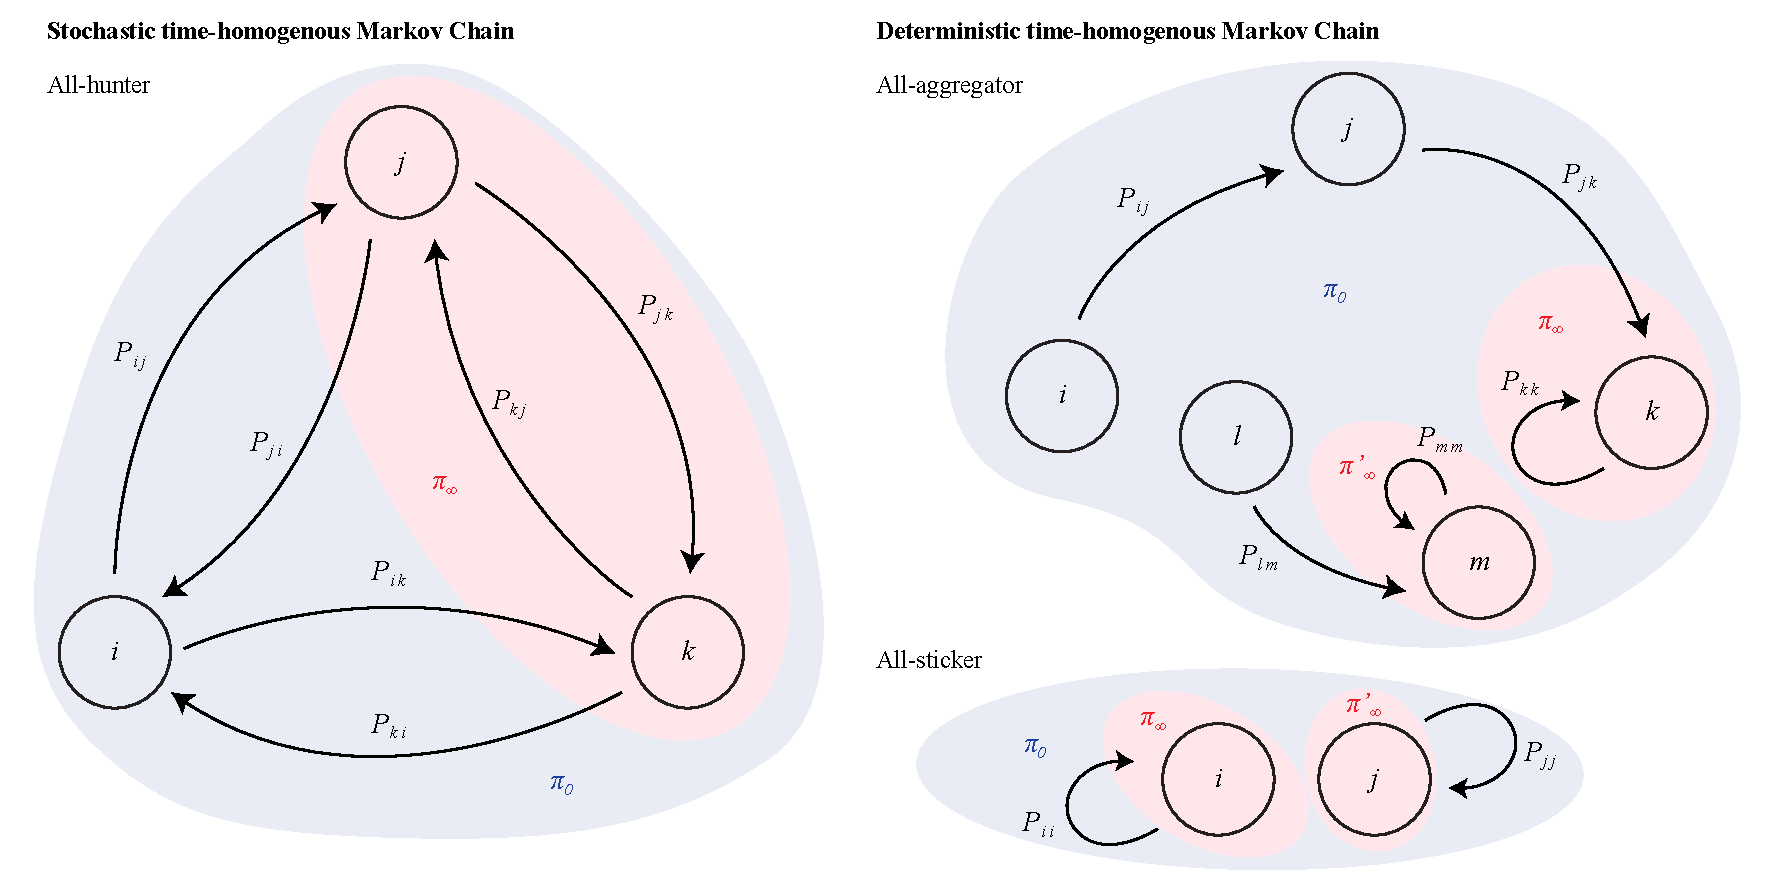
\includegraphics[width=\textwidth]{Graphics/Markov2.pdf}
	\caption{Stylised examples of time-homogenous Markov chains. Each arrow has a corresponding positive \emph{one-step transition probability}, $P_{ij}$ (no arrow indicates that the \emph{one-step transition probability} is zero). The process or \emph{run} starts with an initial state space distribution $\pi_0$, where each element $i$ in the vector $\pi_0$ is the probability of the process starting in state $i$. The process converges to the stationary state space distribution, $\pi_\infty$ (states within the shaded area have positive probability, while states outside have zero probability). The random component in the all-hunter model insures that all \emph{one-step transition probabilities} between different states are strictly positive. A \emph{hunter}-firm never settles down and thus there are no self-loops (the diagonal in the \emph{transition probability matrix}, $\rm P$, consists of zeroes). However the process is ergodic so it converges to a unique stationary state space distribution, $\pi_\infty$, regardless of the initial state space distribution. The all-sticker and all-aggregator model are deterministic THMC, thus all \emph{one-step transition probabilities} equal 1. Both models converge to a single state rather than a distribution of states, since there is no oscillation. However the processes are non-ergodic, and thus the single state depends on the specific probabilities in initial state space distribution $\pi_0$.}
	\label{fig:markov}
\end{figure}

We have argued how a \emph{run} of our model constitutes a stochastic process and linked it to the dynamics of Markov chains. We are now at a point where we can look closer at convergence and steady state. The state space distribution vector is \emph{stationary} when $\pi_{t+1} = \pi_t$. Because of the randomly drawn initial location of firms the initial state space distribution, $\pi_0$, is seldom stationary and several iterations are need. The process reaches steady state once the state space distribution becomes stationary. That is $\lim_{t \to \infty} \pi_t = \pi_\infty$, where the stationary state space distribution, $\pi_\infty$, solves $\pi_{t+1} = \pi_t$. All time-homogenous Markov chains converge to at least one steady state distribution. A process that converges to a unique distribution vector, $\pi_\infty$, regardless of the initial distribution vector, $\pi_0$, is known as an \emph{ergodic} process. There are two types of time-homogenous Markov chains (THMC); \emph{stochastic THMC} that contain a random component (besides the randomly drawn initial positions), and \emph{deterministic THMC} that do not contain any random component and where the probability that the random vector, $Y_t$, takes on a particular values is 1. This distinction is useful since not all THMC are \emph{ergodic}, but as \citet[chapter~4, p.~64]{Laver_Sergenti_2011} note all \emph{stochastic THMC} with a finite state space are \emph{ergodic}. With a random component in the process each state has strictly positive probability of being reached in a finite number of iterations, thus the process avoids ``getting stuck'' and eventually converges to the unique distribution vector \citep[chapter~4, p.~71]{Laver_Sergenti_2011}. Recall that a \emph{hunter}-firm turns around and heads in a randomly selected direction. A random component such as this insures that the process is \emph{ergodic}. We know that this process will converge to a unique state space distribution, $\pi_\infty$, and that this distribution is independent of the initial state space distribution. There is no guarantee that a \emph{deterministic THMC} converges to a single state, since it might oscillate between several states. The deterministic process underlying the all-maxcov model -- where all firms use the \emph{maxcov} decision rule -- does sometimes oscillate between several states. We will deal specifically with this special case in section~\ref{sec:oscmaxcov} -- all other deterministic process in this paper converge to a single state. And all the \emph{deterministic THMC} in this paper are non-ergodic. The arguments for these assertions are provided in \ref{app:overview}. This means that although the process converges to a single state, this state is not unique, but depends on the initial position of firms. The method used to estimate the values of the output variables takes this into account, so our end-results are independent of the initial location of firms.

It is often possible to construct several Markov representations. When choosing the vector of the state space, $X_t$, one need to insure that the output variables, $Y_t$, can be derived from the vector of the state space, i.e. $Y_t = f(X_t)$. In addition the vector of the state space, $X_t$, has to satisfy the Markov property. In most of the models in this paper the vector of the state space only needs to contain the coordinates of the firms, since we can calculate the remaining output variables from the coordinates\footnote{Although the coordinates take on real numbers in theory, in practice when executed on any computer there is a limit to the precision of the coordinates. Matlab stores values using up to 64-bits \citep{MathWorks_2016}. This limited precision is enough for us to say that the coordinates are discrete (to a high level of precision), and thus the state space is finite (although quite large).}. Once the vector of the state space, $X_t$, reaches steady state so will the output variables, $Y_t$.

\subsubsection{Estimating output variables}

We calculate a mean estimate for each of the values in the output variable, i.e. we calculate the mean estimate of the effective number of firms (ENP), the mean eccentricity and the mean representation. We want an accurate estimate of the output variable in steady state, and so none of the output variables obtained in transient states can be used to estimate the steady state. We discard all \emph{burn-in} iterations, that is the iterations needed to reach the steady state. In the subsequent section we return to the empirical issue of determining the number of \emph{burn-in} iterations, but for now assume that the process has burnt in.

Define $\psi_t^{(n)}$ as the expected value of the output variable $Y_t$ at repetition $n$ and iteration $t$. We know that in steady state the state space distribution vector is \emph{stationary}. Thus in steady state the expected values of any of the output variables, $Y_t, Y_{t+1}, Y_{t+2}$, et cetera, must also be stationary, $\psi_t^{(n)} = \psi_{t+1}^{(n)} = \psi_{t+2}^{(n)}$ and so forth, for repetition $n$. Removing the time subscript we have that $\psi^{(n)}$ is the expected value of $Y_t$ for repetition $n$ over all iterations $t$ in steady state. Using this we can define the process of the output variable as the sum of expected value and disturbance term, 

\begin{equation}
Y_t = \psi^{(n)} + \varepsilon_t
\label{eq:process}
\end{equation}

The disturbance term, $\varepsilon_t$, is serially correlated across iterations and therefore indexed with $t$. We execute several repetitions not just repetition $n$. For each repetition we may have a different expected value, i.e. a different value of $\psi^{(n)}$. So we model $\psi^{(n)}$ as the realised value of a random variable, where $\psi^{(n)}$ is drawn from a distribution with mean $\psi$ and standard deviations $\sigma_\psi$. Consequently $\psi$ is the expected value of $Y_t$ over all repetitions and all iterations in steady state. 

To estimate $\psi$ we can use the \emph{ensemble average}. This entails executing several repetitions of a run, up until a pre-specified iteration $t$ that is within the steady state. And then taking the average over all repetitions of the realised values, $y_t^{(n)}$, of the output variable, $Y_t$, at iteration $t$:

\begin{equation}
\mbox{Ensemble Average}_t \mbox{ of } Y_t = \sum\limits_{n = 1}^N {\frac{ y_t^{(n)} }{ N }}
\end{equation}

where $N$ is the total number of repetitions. The ensemble average converges to $\psi$ as the total number of repetitions go to infinity:

$$\psi = \mbox{plim} \sum\limits_{n = 1}^N {\frac{ y_t^{(n)} }{ N }}$$

The disadvantage of using the \emph{ensemble average} to estimate $\psi$ is that we discard a lot of \emph{burn-in} iterations. For instance if we determine that it takes 251 iterations for the process to burn in and we execute 100 repetitions. Then the first 250 \emph{burn-in} iterations in each repetition are of no use when estimating the output variables in steady state. In total we discard 25,000 iterations and only use information from 100 iterations (the last iteration in each repetition) in our estimate. By any stretch this is a highly ineffective use of computational resources. For this reason, when possible, we would prefer to use the \emph{time average} to estimate $\psi$. This entails executing a single repetition of a run, up until a pre-specified number of post-burn-in iteration. And then taking the average of $y_t^{(n)}$ over all post-burn-in iterations:

\begin{equation}
\mbox{Time Average}^{(n)} \mbox{ of } Y_t = \sum\limits_{t = 1}^T {\frac{ y_t^{(n)} }{ T }}
\end{equation}

where $T$ is the total number of post-burn-in iterations and all iterations, $t \in \{1,2, \dots, T\}$, are within the steady state. As the total number of iterations go to infinity, the time average converges to $\psi^{(n)}$, i.e. the expected value of $Y_t$ for repetition $n$. Recall that an \emph{ergodic} process converges to the same unique state space distribution regardless of the initial distribution. And since the only difference between different repetitions within the same run is the initial positions of firms, it implies that the limiting state space distribution is independent of the particular repetition when the process is \emph{ergodic}. So for a \emph{ergodic} process we have that $\psi^{(n)}$ is equal to $\psi$, in which case:

$$\psi = \mbox{plim} \sum\limits_{t = 1}^T {\frac{ y_t^{(n)} }{ T }}$$

Recall the example from above where it takes 251 iterations for the process to burn in. We further assume that the process is ergodic and execute 100 post-burn-in iterations. Using the time average we execute a single repetition with an overall of 351 iterations. In total we only discard 250 \emph{burn-in} iterations, and use information from the last 100 iterations to estimate $\psi$. In this example we reduced the number of discarded iterations by a factor 100 when using the \emph{time average} instead of the \emph{ensemble average}. However with a high degree of autocorrelation in the process it might not be possible to use the \emph{time average} -- which is what we show below. Further note that all our \emph{deterministic time-homogenous Markov chains} are non-ergodic, so for these processes we have no other option, but to use the \emph{ensemble average} to estimate $\psi$.

The disturbance term in equation~\ref{eq:process} is independent and identically distributed (IID) across repetitions, because we use a different random seed for each repetition. As previously noted different random seeds give different sequences of numbers, and these sequences are IID, which in turn produce disturbance terms that at any given iteration are IID across repetitions. So when executing several repetitions the observed values at iteration $t$ will be reasonably equally spread around the true mean, and the \emph{ensemble average} gives a representative mean estimate of $\psi$. The \emph{time average} may not give a reasonably representative estimate, because the disturbance term is serially correlated across iterations. While an ergodic process will eventually map out the entire steady state distribution vector, $\pi_\infty$, the process is slow to map out the distribution if there is a high degree of autocorrelation. A fully mapped out distribution assures that the \emph{time average} gives a representative estimate of $\psi$. To check whether enough observations have been collected to map out the steady state distribution vector we run several test repetitions. For each output variable we calculate the \emph{R-hat statistic}\footnote{The \emph{R-hat statistics} is also known as the \emph{potential scale reduction factor}. When running our test repetitions we calculate the \emph{R-hat statistic} using the second half of all iterations.} \citep{Laver_Sergenti_2011, Brooks_Gelman_1998}. The R-hat statistic is a relative measure of the between-repetition variance and the total within-repetition variance. And thus the measure reveals whether there is a potential to trim the state space distribution further by increasing the number of iterations. A low R-hat statistic indicates less potential to trim. In the limit the R-hat statistic tends to 1. This paper uses the typical cutoff level of 1.05. If the R-hat statistic for every output variable is lower than 1.05, then we feel confident that the steady state distribution has been mapped out and proceed to using the \emph{time average} in the final execution of the model. If the R-hat statistic is above 1.05 we can try to increase the number of iterations and re-run the test, or we will determine that the speed of convergence is prohibitively slow and resort to using the \emph{ensemble average} in the final execution of the model. In the following section we distinguish between \emph{stochastic THMC} where the \emph{time average} provides a representative estimate of $\psi$ and those that do not, i.e. whether the R-hat statistic is below the cutoff level for all the output variables, or not. 

\begin{figure}[hb!]
	\caption{Example of trace plots.}
	\centering
	\begin{subfigure}[t]{0.485\textwidth}
		\includegraphics[width=\textwidth]{Graphics/figb21a.pdf}
		\caption{A single repetition from a deterministic THMC. This repetition burns in after 12 iterations, where mean eccentricity flatlines.}
		\label{fig:deterministic}
	\end{subfigure}
	~
	\begin{subfigure}[t]{0.485\textwidth}
		\includegraphics[width=\textwidth]{Graphics/figb22a.pdf}
		\caption{A single test repetition from a stochastic THMC. Solid black line is the \emph{time average} calculated using the second half of all iterations. Dotted black lines indicate $\pm$ one standard deviation. Burns in after 61 iterations (estimate within one standard deviation of estimate).}
		\label{fig:stochastic}
	\end{subfigure}
	\label{fig:traceplots}
\end{figure}

\subsubsection{Determining burn in}

We want an estimate of our output variables in steady state. So for each model we need to empirically determine the number of \emph{burn-in} iterations. For a deterministic THMC this is fairly straightforward, when the process converges to a single state. The process has burnt in once the values no longer change, i.e. once the process becomes stationary. Empirically we set the \emph{burn-in} period to the maximum number of iterations it takes before the output variables flatline, see figure~\ref{fig:deterministic}\footnote{For each repetition we find the first iteration where the value of the output variable is equal to the value at the last iteration. From all the repetitions we select the largest of these iterations. This is then the number of iterations needed for all the repetitions in the model to burn in.}. A stochastic THMC converges to a distribution of states rather than a single state (see example in figure~\ref{fig:stochastic}), which make it slightly more difficult to empirically determine burn in. In the processes where the \emph{time average} provides a representative estimate of $\psi$ we first identify the runs that require most iterations to converge -- so called extreme cases. This is done by executing a few repetitions from different runs (i.e. different parameter values) of the model and then visually inspecting the trace plots of the output variables\footnote{A trace plot displays the iterative history of a repetition, i.e. the time series of one value of the vector $y_t^{(n)}$ by iteration, such as mean eccentricity by iterations or ENP by eccentricity etc.}. Secondly, we execute several test repetitions with many iterations of these extreme cases. We focus on the extreme cases, since we want to find the number of \emph{burn-in} iterations needed for all runs of the model to reach steady state. For each test repetition we calculate the \emph{time average} and corresponding standard deviation using the second half of all iterations\footnote{The second half procedure is a sufficient although not a necessary condition for the process to burn in \citep[chapter~4, p.~73]{Laver_Sergenti_2011}. We use this procedure to get a representative estimate of $\psi$, when we have yet to determine the actual number of \emph{burn-in} iterations.}. And finally, with our estimate of $\psi$ we determine that a particular test repetition has burnt in once the output variable is within one standard deviation of the estimated $\psi$, see figure~\ref{fig:stochastic}. We set the \emph{burn-in} period to the maximum number of iterations it takes for each of the test repetitions to burn in. In the stochastic THMC where the \emph{time average} does not provide a representative estimate of $\psi$, the first two steps are unchanged; first identify runs that require most iterations to converge, and secondly execute several test repetitions. However since we cannot use the \emph{time average} to calculate a representative estimate of $\psi$ we must rely on a less rigorous method to determine the number of \emph{burn-in} iterations. For every test repetition we visually inspect the trace plots of each of the output variables to determine when the test repetition appears to have reached steady state, see example in figure~\ref{fig:filtertime}. We set the \emph{burn-in} period to the maximum number of iterations it takes for each of the test repetitions to burn in. In the final execution of all our models we choose to err on the side of caution and set the \emph{burn-in} period slightly higher -- often rounding up to the nearest fifty, i.e. 50, 100, 150,~etc.

\begin{figure}[htp!]
	\caption{Example of multiple test repetitions. To ease the inspection of multiple test repetitions required developing a small interactive tool, see \url{https://github.com/jsekamane/filter-time}. The tool displays all repetition in the same trace plot, with the option to highlight a specific repetition or all repetitions with a specific combination of parameter values. As well as the option to standardise the series. These figures are derived from the tool.}
	\centering
	\begin{subfigure}[t]{0.83\textwidth}
		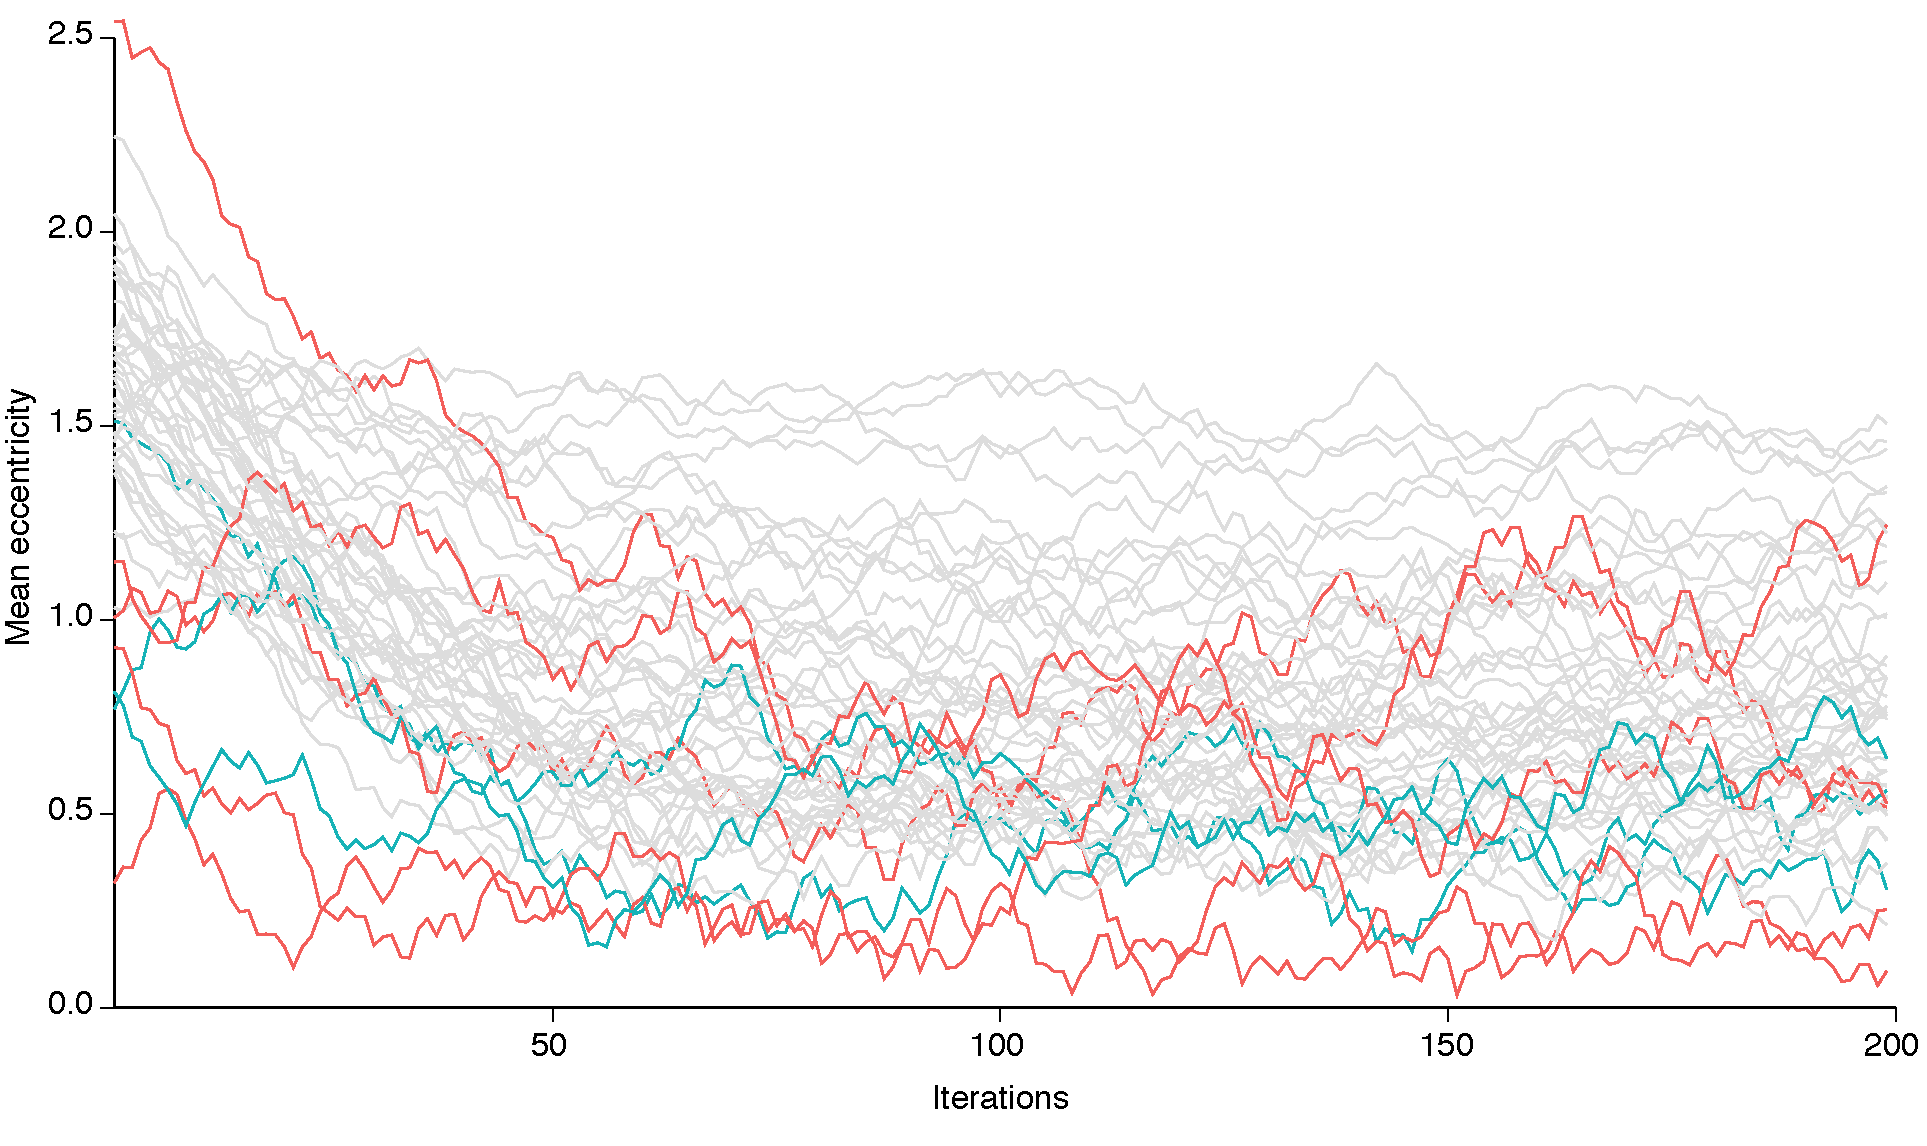
\includegraphics[width=\textwidth]{Graphics/figb23a.pdf}
		\caption{Multiple test repetitions from different runs (i.e. different parameter values). Red and blue highlights are repetitions with respectively 2 and 3 firms.}
		\label{fig:multirep}
	\end{subfigure}
	
	\begin{subfigure}[t]{0.83\textwidth}
		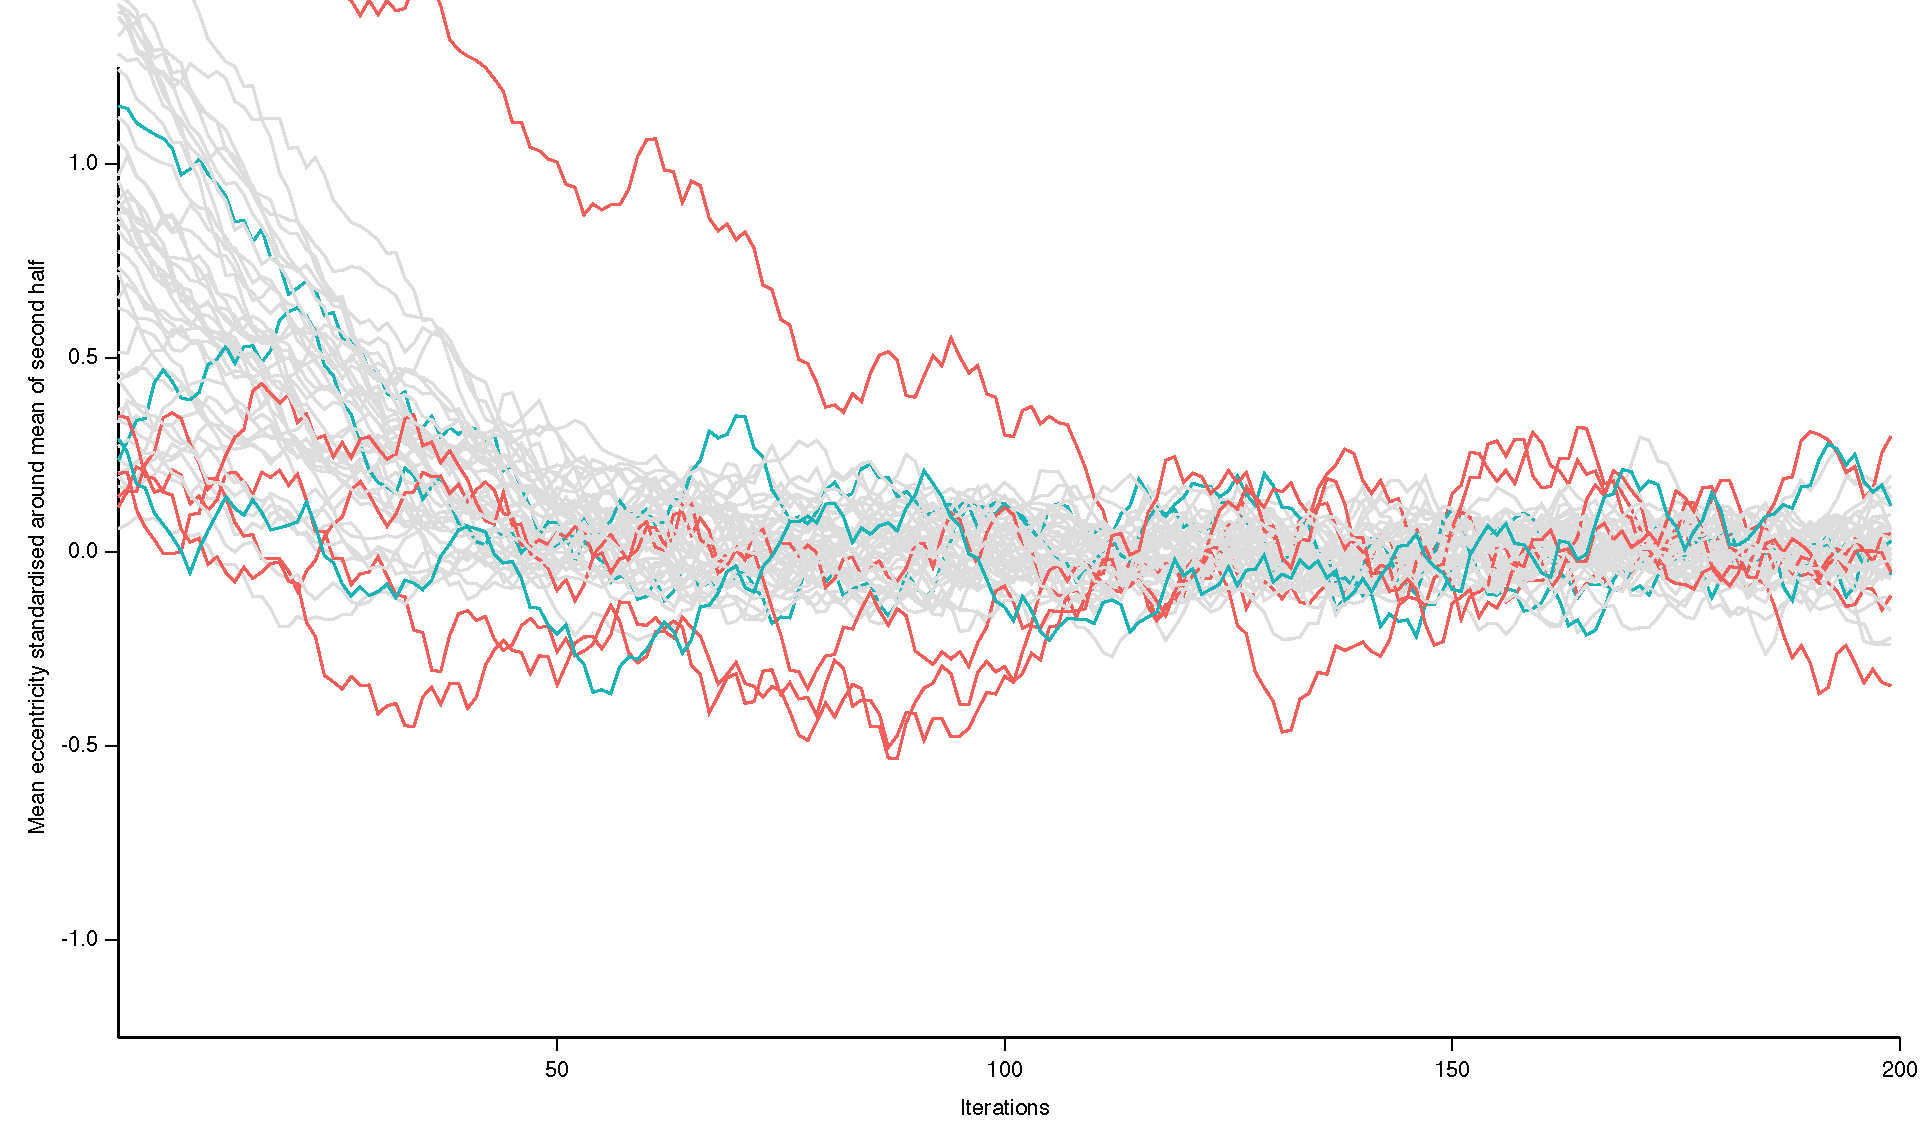
\includegraphics[width=\textwidth]{Graphics/figb23b.pdf}
		\caption{Mean eccentricity is standardised around the mean of the second half of all iterations. Standardising helps determine burn in, especially when considering different runs with different combination of parameter values. Clearly the repetitions with 2 and 3 firms require most iterations to burn in. This model appears to have reached steady state after approximately 150 iterations.}
		\label{fig:multirepstd}
	\end{subfigure}
	\label{fig:filtertime}
\end{figure}


\subsubsection{Oscillation in all-maxcov model}
\label{sec:oscmaxcov}

The all-maxcov model, where all firms use the \emph{maxcov} decision rules, is a deterministic THMC. However unlike the other deterministic THMC, this process does not necessarily converge to a single state. For certain parameter values and initial locations of the firm the process oscillates between several states. If the process oscillates between many vastly different states, then calculating the ensemble-average at iteration $t$ is unlikely to provide a representative estimate of $\psi$. And because the process is non-ergodic -- the distribution vector, $\pi_\infty$ depends on the initial distribution vector, $\pi_0$ -- the time-average will not provide a representative estimates of $\psi$ either. Instead we assume that the process oscillates between a few states where the location of firms only differ slightly, and then calculate the ensemble average. We create a new decision rule called \emph{maxcovrnd} with one slight modification: instead of moving 0.1 standard deviation, the firm randomly draws the speed parameter for a uniformly distribution with range $[0,0.2]$. On average the firm moves 0.1 standard deviation. But more importantly the process contains a random component, and so it constitutes a \emph{stochastic THMC}, where we know with certainty that the ensemble average provides a representative estimate of $\psi$. When we compare the results of the all-maxcov model to the all-maxcovrnd model we find that the results are minuscule (see \ref{app:maxcovrnd}). This confirms that the deterministic process does in fact oscillates between a few slightly different states. And so we feel confident that using the ensemble-average in the all-maxcov model provides representative mean estimates of our output variable. We prefer to use the \emph{maxcov}-rule, rather than the \emph{maxcovrnd}-rule, since we are going to extend the model with firms that try to predict the future location of the other firms. Evaluating predictions makes less sense when the location of firms contains a stochastic component.

\subsubsection*{Recap}

In sum we have constructed an experimental design that allows us to evaluate the effect of parameter changes, and insures that results are independent of the initial position of firms. We have identified the appropriate methods to estimate the summary variables. The appropriate method depend on the underlying process, see outline in figure~\ref{fig:process}. Understanding the underlying process of the run provides us with prior knowledge on how we should go about solving the model. However it still requires some effort and test repetitions to determine the number of \emph{burn-in} iterations and to determine whether the \emph{time average} provides representative estimates. Once this has been determined the final execution of the model is straightforward.

\begin{figure}[ht]
	\centering
	\includegraphics[width=\textwidth, trim={16mm 15mm 19mm 20mm},clip]{Graphics/Process.pdf}
	\caption{Outline of the various processes and their respective requirements. The respective methods used to estimate $\psi$ are presented furthest to the right.}
	\label{fig:process}
\end{figure}


\section{Analysis}

We are now ready to investigate the first models. We start with the all-sticker, all-aggregator, all-hunter and all-maxcov models. In each of these models all the firms use the same decision rule. Unlike \citet{Fowler_Laver_2008} that run a tournament to determine the best preforming decision rules, we want to analyse the underlying dynamics of each decision rule and how these different decision rules affect the location behaviour of firm. By comparing results across the four different models, we see how the location behaviour of the decision rules differ. We start with a symmetric unimodal distribution of consumers. The peak of the consumer distribution function coincides with the mean ideal point of all consumers. There is no polarisation of the mean ideal points of the two subpopulations and the subpopulations are equally large ($\mu=0$ and $n_l/n_r=1$). Thus there is the only one free parameter in each model; the number of firms $N$. We use the grid sweep method to set this parameter value.

\subsection{Baseline model and decision rules}

\begin{figure}[ht!]
	\centering
	\includegraphics[width=\textwidth]{Graphics/fig21a.pdf}
	\caption{Mean eccentricity for respectively all-sticker, all-aggregator, all-hunter and all-maxcov model. Where $\mu=0$ and $n_l/n_r=1$.}
	\label{fig:eccentricity}
	\Fignote{All models use grid sweep method, i.e. each model executes 11 runs (one for each value of $N$). The all-sticker, all-aggregator and all-maxcov model uses the \emph{ensemble average}, and is executed with 1,000 repetitions, and respectively 1, 50, 99 burn-in iterations. The all-hunter model uses the \emph{time average}, and is executed with 1 repetition and 1,150 iterations (burn-in after 150 iterations). The bands indicate the 95\% confidence interval of our estimate.}
\end{figure}

In the all-sticker model the firms remain at their initial position. They never relocate. Figure~\ref{fig:eccentricity} plots the mean eccentricity for all four models. As expected we see that the average distance to the population centre is 1.5 standard deviation in the all-sticker model. This result reflects how the initial positions of firms are drawn, i.e. uniformly random from a circle with radius of 3 standard deviations and centre at (0,0). And thus we find that on average a \emph{sticker} firm will be located 1.5 standard deviations from the centre of the population -- irrespective of the number of firms in the market. In the three remaining models mean eccentricity is significantly lower. The initial position of the firms in these models are drawn from exactly the same distribution, but the firms clearly moved towards the population centre. 

In the all-aggregator model the firms aim to please their current customer base. The firms choose to locate 0.4-0.8 standard deviations away from the population centre with the distance increasing along with number of firms in the market. In the all-hunter model, where all firms constantly seek higher market shares, the firms choose to locate in closer proximity to the population centre than in the all-aggregator model. \emph{Hunter} firms locate around 0.2 standard deviation closer to the centre than \emph{aggregator} firms.

\piccaption{\label{fig:marketshare} Eccentricity against market share for each firm. This shows the results from a single repetition with 5 \emph{hunter} firms. At each iteration we record the eccentricity and market share of each firm. We smoothed the data. The estimated mean eccentricity for five \emph{hunter} firms is 0.44 standard deviations vertical red line).}
\parpic[l]{\includegraphics[width=0.5\textwidth]{Graphics/fig3ms.pdf}}

Despite the fact that the population centre has the largest density of consumers of any point in the market, firms consistently locate at a distance to this point — even \emph{hunter} firms that constantly seek larger market shares. This suggests that locating too close to the population centre is suboptimal \citep[chapter~5]{Laver_Sergenti_2011}. For a \emph{hunter}-firm there is a short-run gain by moving closer to the high density population area. However the response from competing firms quickly erodes this gain, leading to the long-run location that lies at a distance to the population centre. Our estimate of mean eccentricity for five \emph{hunter} firms is 0.44. Compare this to figure~\ref{fig:marketshare}, where we for each of the five \emph{hunter} firms plot eccentricity against market share. When the individual firm locates 0.44 standard deviations from the population centre, its share of the market is around 21\%. Locations closer to the population centre is associated with a higher share of the market for each individual firm, i.e. a short-run gain. However all firms use the same disunion rule and thus no one firm has a long-run competitive advantage over its competitors. In the long-run the firm cannot sustain the larger market share, leading to the long-run location at a distance to the population centre.

In the all-maxcov model the firms deliberately attempt to maximise their market share. And the firm takes the location of competing firms into account, although it assumes that competing firms maintain their current position. Firms in the all-maxcov and all-hunter model locate at similar distance to the population centre, except in the market with two firms. In this case the \emph{maxcov} firms locate at the same distance as \emph{aggregator} firms. Recall that a \emph{maxcov}-firm locates in the largest Delaunay triangle. When there are two firms in the market, then each firm chooses among four triangles. All these triangles have a common corner at the location of the competing firm\footnote{The edge opposite the common corner in each triangle is the respective edges of the boundary of the space. The \emph{maxcov} decision rule does not consider corner solutions, i.e. locating at the exact same location as competing firms, but assumes that the ideal location lies between the gaps of competing firms. When faced with only one competing firm, then there is no gap and the \emph{maxcov} firm move towards one of four points surround the competitor. Note however that the \emph{maxcov} firm always move towards the side of the competitor with the largest share (i.e. largest half market).}. When the competing firm locates reasonable close to the population centre, then only a small fraction of most densely populated area is contained within each triangle. And, since the \emph{maxcov}-firm locates at the mean ideal point of all consumers within the triangle, this implies that centre of mass of the triangle is shifted slightly away from the population centre. This is why the estimated mean eccentricity is 0.4 standard deviations in the all-maxcov model with two firms. In the all-maxcov model there is only a slight tendency for firms to locate further away from the population centre as the number of firms increase. On average the \emph{maxcov}-firms locate 0.4-0.5 standard deviations away from the population centre.

\TODO{Compare results to \citet{Eaton_Lipsey_1975} / equilibrium predictions (two firms).}

\begin{figure}[ht!]
	\centering
	\includegraphics[width=\textwidth]{Graphics/fig22a.pdf}
	\caption{Effective number of firms (ENP) for respectively all-sticker, all-aggregator, all-hunter and all-maxcov model. Where $\mu=0$ and $n_l/n_r=1$.}
	\label{fig:enp}
\end{figure}

In the models the actual number of firms in the market is an endogenously determined parameter. Our experimental design allows us to investigate the models when there is anywhere from 2 to 12 firms in the market. To analyse the competitive environment we use a measure called \emph{effective number of firms} (ENP). The ENP takes the relative market shares of the firms into account. The ENP tells how many firms would be in the market if they all had identical shares of the market. If the actual number of firms and the effective number of firms is the same (grey diagonal line in figure~\ref{fig:enp}), then the firms in the market split the market evenly. If the effective number of firms is less than the actual number, then one or several of the firms will have a disproportionate share of the market.

The effective number of firms is low in the all-sticker model, ranging from around 1.5 and up to 4.5. The initial position of firms gives some firms a clear advantage over the other firms in the market. And since \emph{sticker} firms do not relocate the uneven concentration of customers persists.

In the last three models the market is fairly evenly split among the firms. \TODO{This is the result of firms with identical decision rules competing with one another. Since all firms use the same decision rule, no one firm has a long-run advantage over its competitors. And thus the firms end up with a fairly even share of the market in the long-run.} With many firms in the market it is increasingly harder to maintain the perfectly even split among the firms. And so we observe that the ENP increases slower than the number of firms in the market increases.

In the all-aggregator model with many firms the effective number of firms is slightly lower than the all-hunter and all-maxcov model. The reason for this is that with many firms the centre of the distribution easily overcrowds. \emph{Aggregator}-firms locate to please their current customer base. And so overcrowding leads the firms to locate on different orbits around the centre. Firms located on the inner orbits attract a larger share of the consumers than the firms located on the orbits further away from the centre. And the unequal market share of firms reduces the \emph{effective number of firms} (ENP).

\begin{figure}[ht!]
	\centering
	\includegraphics[width=\textwidth]{Graphics/fig23a.pdf}
	\caption{Mean representation for respectively all-sticker, all-aggregator, all-hunter and all-maxcov model. Where $\mu=0$ and $n_l/n_r=1$.}
	\label{fig:representation}
\end{figure}

The mean representation measures the satisfaction of consumers. This social welfare measure calculates the average utility of all consumers. The utility of the consumer increases when the distance to the closest firm decreases. From earlier we known that the all-aggregator model will result in the location of firms that constitute a \emph{Centroidal Voronoi Tessellation} (CVT). The CVT minimises the average distance to all customers and therefore maximises our social welfare measure. The all-aggregator model provide a benchmark, since the location of firms is socially optimal.

In both the all-hunter and all-maxcov model where firms aim to maximise their market share, they manage to achieve almost the same mean representation as in the all-aggregator model, where firms actively aim to please their customer base. And this despite \emph{hunter} and \emph{maxcov}-firms locating closer to the population centre than \emph{aggregator}-firms. We also see that as the number of firms in the market increases the mean representation converges towards the social optimal level. Unsurprisingly the all-sticker model scores lowest on our social welfare measure.

\subsection{Asymmetric and multimodal population distribution}

In the section above we got a sense of the different models and how firms react when using different decision rules. Our results have so far assumed a symmetric unimodal distribution of consumers. There was no disagreement between the two subpopulations over the average ideal point along any of the two dimensions. There was a single peak in the aggregated distribution where the density of consumers was greater than any other point, and the peak corresponded to the mean ideal point of all consumers. We observed that firms chose to locate at a distance to mean ideal point of consumers. The literature review showed that different distributions of consumers have had significant impact on the results of previous competitive location models. We now want to investigate how firms locate when there is not a single peak in the distribution? How the location dynamics of firms change when the subpopulations disagree over the mean ideal point? And to what extend our results so far generalise to other distributions, such as the asymmetric and multimodal distributions? 

We continue to investigate models where all firms use the same decision rule. Firms are competing against other firms using the same decision rule. Firms using the \emph{sticker}-rule do not relocate, and thus executing the all-sticker model with an asymmetric consumer distribution would not provide further insights. Thus we disregard the \emph{sticker} decision rule in this subsection. 

In the following models there are three free parameters; The number of firms in the market $N$ which takes integer values between 2 and 12. The polarisation of the subpopulations $\mu$ which can take any value between 0 and 1.5. And finally the relative size of the subpopulation $n_l/n_r$ which takes any value between 1 and 2. To parametrise our models we use the Monte Carlo parameterisation method. For each run of the model the parameter values are uniformly random drawn from their respective ranges. We execute many \emph{runs} of the models to map out the entire parameter space. For each run we obtain a mean estimate of our summary variables. In the following figures each dot represents the estimate from one run. We present the results from the different decision rules in separate panels. \TODO{We use three bands to summarise the results from different degrees of polarisation among the subpopulations}. The first band summarises the results from the runs where there is a low degree of polarisation ($\mu \le 0.5$). We know from earlier, that this implies, that the distribution of consumers contain a single peak, and that the degree of asymmetry depends on the relative size of the subpopulation. The second band is for a medium degree of polarisation ($0.5 < \mu < 1$). And the last band is for a high degree of polarisation ($\mu \ge 1$). In this range we know that the distribution is bimodal and that the peaks of the distribution almost coincide with the mean ideal points of the two subpopulations. In addition the mean ideal point of all consumers lies in the low density area in between the two peaks.

\begin{figure}[ht!]
	\centering
	\caption{Mean eccentricity where $\mu \in [0, 1.5]$ and $n_l/n_r \in [1, 2]$.}
	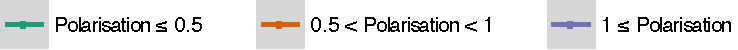
\includegraphics[width=90mm]{Graphics/legend_pol.pdf}

	\begin{subfigure}[t]{0.315\textwidth}
		\includegraphics[width=\textwidth, trim={8mm 0 0 0}]{Graphics/fig331a_tall.pdf}
		\caption{All-aggregator}
		\label{fig:eccentricity_aggregator}
	\end{subfigure}
	~
	\begin{subfigure}[t]{0.315\textwidth}
		\includegraphics[width=\textwidth, trim={8mm 0 0 0}]{Graphics/fig321a_tall.pdf}
		\caption{All-hunter}
		\label{fig:eccentricity_hunter}
	\end{subfigure}
	~
	\begin{subfigure}[t]{0.315\textwidth}
		\includegraphics[width=\textwidth, trim={8mm 0 0 0}]{Graphics/fig341a_tall.pdf}
		\caption{All-maxcov model}
		\label{fig:eccentricity_maxcov}
	\end{subfigure}
	
	\label{fig:asymetric_eccentricity}
		\Fignote{All models use Monte Carlo parameterisation method, the \emph{ensemble average}, and is executed with 500 runs. The all-aggregator model is executed with 100 repetitions and 100 burn-in iterations. The all-hunter model with 100 repetitions and 150 burn-in iterations. The all-maxcov model with 50 repetitions and 150 burn-in iterations. For each of the three degrees of polarisation the respective estimates are smoothed using the \emph{local polynomial regression fitting} (LOESS) method, with the bands indicating the corresponding 95\% confidence interval.}
\end{figure}

Firms using the \emph{hunter}-rule still locate closer to the mean ideal point of consumers than the firms using the \emph{aggregator}-rule for any degree of polarisation. However the differences in proximity between \emph{hunter}-firms and \emph{aggregator}-firms is much less pronounced in markets with a high degree of polarisation and many firms. Here the mean eccentricity is approximately 1.2-1.4 for both decision rules.

In the highly polarised setting we see significant differences between the market with 4 or more \emph{hunter}-firms and then the market with 2 or 3 \emph{hunter}-firms. For one we see that the distance to the mean ideal point of consumers increases swiftly when going from two to three and from three to four firms. While going beyond four firms in the market has negligible effect on the average distance to the population centre. This happens because firms separate when there is four or more firms in the market. In these cases we typically see that firms split into two crowds. Each crowd locates close one of the peaks of the consumer distribution function. The number of firms in each crowd is roughly proportional to the relative size of the subpopulation. There is little competition between firms from different crowds, while the firms in each crowd compete fiercely with one another for the customers in the respective subpopulation. In the symmetric all-hunter model (discussed in the previous subsection) with four or more firms in the market, we observed that firms locate 0.4–0.6 standard deviations away from the peak of the distribution. Similar behaviour is observed in the models with a high degree of polarisation, however here we have two peaks rather than one. And the firms tend to locate around a peak, rather than in between the two peaks. See an example of this split in a market with five firms in figure~\ref{fig:movement}. Each individual \emph{hunter} firm experiences a short-run loss when it moves away from a peak. This discourages the firm from switching between the crowds. Thus the composition of the crowd is fairly stable, and the firm sees no long-run advantage in locating between subpopulations and close to the mean ideal point of all consumers. On the other hand with two or three \emph{hunter}-firms in the market, the firms tend to move in unity\footnote{Because \emph{hunter} firms cannot leapfrog to the perimeter, but move with constant speed, we don't observe the \emph{dancing equilibrium} described \citet{Eaton_Lipsey_1975} in the market with three \emph{hunter}-firms. Instead the three firms move in unity and the location of the unit bounces back and forth between the two peaks of the distribution.}. Two \emph{hunter} firms tend to locate in between the two subpopulations. Thus they locate close to the average ideal point of all customers, but simultaneously they locate in an area with a low density of consumers. Later we show that this has great impact on the average utility of consumers. With two firms and little to no polarisation, all decision rules show that the firms locate within 0.6 standard deviation of the mean ideal point of all consumers. However only \emph{hunter}-firms continue to locate like this when the polarisation among the subpopulation increases. This effect shows the interplay of decision rule and the distribution of consumers.

\citet[chapter~5]{Laver_Sergenti_2011} discovered the change when going from 2-3 \emph{hunter} firms and into the realm of four or more \emph{hunter} firms. Yet they seem unaware of an earlier and related discovery by \citet{Eaton_Lipsey_1975}. \citet{Eaton_Lipsey_1975} also analyse asymmetric distributions admittedly in a slightly different setting, namely the bounded one-dimensional space (line market). They show analytically that an equilibrium only exists if the number of firms is less or equal to twice the number of peaks in the density distribution, i.e. $N \le 2M$ where $M$ is the number of peaks in the consumer density function. They find that when the number of firms is exactly twice the number of peaks then the firms locate in pairs around the quantiles of the distribution. While with fewer firms (than twice the number of peaks) there is some leeway as to how firms locate. Both the pairing of firms in groups of two and the $2M$ limit stems from the single dimensionality of the space. In a one-dimensional line market the only available option is which side of a given point you locate on (left or right). Using this and equilibrium conditions \citet{Eaton_Lipsey_1975} show the limit of $N \le 2M$. In the two-dimensional market firms can locate 360 degrees around a given point, and thus firms need not pair in twos. This is what we observe in the all-hunter model where firms crowd together although not necessarily in pairs of two. Additionally in two-dimensional space the number of peaks does not create an upper limit on the number of firms in the crowd -- once again because firms can locate all the way around a given point. But the number of peaks does seem to influence how firms locate. There is a single peak in the model with a symmetric distribution, and two peaks with highly polarised subpopulations. Only when the number of firms is equal or greater than the number of peaks do the \emph{hunter} firms form crowds around the peaks of the distributions. When the number of firms is less than the number of peaks, then there is some leeway as to how firms locate and thus we see that \emph{hunter} firms locate between the peaks of distribution. I strongly suspect that consumer distribution with three peaks and five or less \emph{hunter} firms would give some leeway as to how firms locate. With four peaks, seven or less firms would have leeway as how to locate, etc.

The symmetric distribution showed that \emph{maxcov} and \emph{hunter} firms locate at similar distance to the population centre, except with two firms in the market. We see similar pattern with the asymmetric distribution of customers. The \emph{maxcov} and \emph{hunter} firms locate a similar distance to the population centre irrespectively of the polarisation of the subpopulations. The exception is when there are only a few firms in the market. With the \emph{maxcov} decision rule there is no abrupt change when going from 2-3 firms and to 4 or more firms, as is the case with the \emph{hunter} decision rule. \emph{Maxcov}-firms separate in two crowds even in the case with low or no polarisation of the subpopulations. Two \emph{maxcov} firms will not agglomerate at the average ideal point of all customers, but instead locate at a distance to the centre. This contrasts starkly with the two \emph{hunter} firms that agglomerate around the population centre.

\begin{figure}[ht!]
	\centering
	\caption{Effective number of firms (ENP) where $\mu \in [0, 1.5]$ and $n_l/n_r \in [1, 2]$.}
	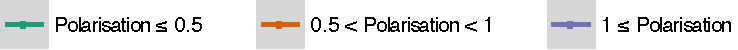
\includegraphics[width=90mm]{Graphics/legend_pol.pdf}
	
	\begin{subfigure}[t]{0.315\textwidth}
		\centering
		\includegraphics[width=\textwidth, trim={8mm 0 0 0}]{Graphics/fig332a_tall.pdf}
		\caption{All-aggregator}
		\label{fig:enp_aggregator}
	\end{subfigure}
	~
	\begin{subfigure}[t]{0.315\textwidth}
		\centering
		\includegraphics[width=\textwidth, trim={8mm 0 0 0}]{Graphics/fig322a_tall.pdf}
		\caption{All-hunter}
		\label{fig:enp_hunter}
	\end{subfigure}
	~
	\begin{subfigure}[t]{0.315\textwidth}
		\centering
		\includegraphics[width=\textwidth, trim={8mm 0 0 0}]{Graphics/fig342a_tall.pdf}
		\caption{All-maxcov model}
		\label{fig:enp_maxcov}
	\end{subfigure}
	
	\label{fig:asymetric_enp}
\end{figure}

The asymmetric distribution reiterates the conclusions from the symmetric distribution regarding the effective number of firms (ENP). Both the model with \emph{aggregator} and \emph{hunter} firms show that the market is relatively even split among the firms in the market. When there are many firms and a low degree of polarisation then the ENP is slightly lower in the \emph{aggregator} model than the \emph{hunter} model. As mentioned when discussing the symmetric model, with many firms in the market the area around the single peak easily overcrowds, and thus \emph{aggregator} firms locate at different orbits around the peak. This gave rise to the slightly lower ENP in the \emph{aggregator} model. When the degree of polarisation increases the density of consumers is dispersed across a larger area, which leads to less overcrowding. Consequently \emph{aggregator} firms are no longer forced to locate at different orbits, which implies that the market is more evenly split among firms. This is why the difference in ENP completely disappears as the polarisation of the subpopulations increase.

The market is also relatively even split among the firms in the \emph{maxcov} model. In the market with many firms and a high degree of polarisation the ENP is slightly lower. As earlier noted the firms split into two crowds in the \emph{maxcov} model. However in the \emph{maxcov} model the number of firms in each crowd is not necessarily proportional to the relative size of the subpopulations. Often a few firms manages to capture one-half of the market and this results in the lower ENP. The ENP would be 3.6 if a single firm out of 12 firms captured half the market\footnote{Calculated using equation~\ref{eq:enp}. With N=12 and the market split in two halves the ENP is $\frac {(0.5+0.5)^2}{\left(\frac{0.5}{11}\right)^2 \times 11 + 0.5^2} = 3.6$ when 1 firm has 50\% of the market and the 11 other firms share the remaining 50\% equally.}. However with 12 firms in the market we observe an ENP around 10. This tells us that a single firm is unable to capture and maintain half the market by itself in the long-run -- it has to be a group of firms.

\begin{figure}[ht!]
	\centering
	\caption{Mean representation where $\mu \in [0, 1.5]$ and $n_l/n_r \in [1, 2]$.}
	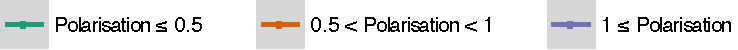
\includegraphics[width=90mm]{Graphics/legend_pol.pdf}
	
	\begin{subfigure}[t]{0.315\textwidth}
		\centering
		\includegraphics[width=\textwidth, trim={8mm 0 0 0}]{Graphics/fig333a_tall.pdf}
		\caption{All-aggregator}
		\label{fig:representation_aggregator}
	\end{subfigure}
	~
	\begin{subfigure}[t]{0.315\textwidth}
		\centering
		\includegraphics[width=\textwidth, trim={8mm 0 0 0}]{Graphics/fig323a_tall.pdf}
		\caption{All-hunter}
		\label{fig:representation_hunter}
	\end{subfigure}
	~
	\begin{subfigure}[t]{0.315\textwidth}
		\centering
		\includegraphics[width=\textwidth, trim={8mm 0 0 0}]{Graphics/fig343a_tall.pdf}
		\caption{All-maxcov model}
		\label{fig:representation_maxcov}
	\end{subfigure}
	
	\label{fig:asymetric_representation}
\end{figure}

In the \emph{aggregator} model where the distribution of consumers is asymmetric, the location of firms still constitute a CVT. And thus this model maximises our social welfare measure -- the mean representation. Once again we can use the \emph{aggregator} model as a benchmark. The difference between the mean representation in the \emph{aggregator} model and the \emph{maxcov} model is minuscule.

In the \emph{hunter} model we see that the asymmetric distribution of consumers give rise to significant changes when going from 2-3 firms and to 4 or more firms. This is particularly pronounced in the models with a high degree of polarisation. With two or three \emph{hunter} firms the mean representation is around -2, while with four or more firms the mean representation is between -0.5 and -0.2. As earlier noted this is the result of \emph{hunter} firms locating in between the centres of the subpopulations when there are 2-3 firms in the market. Although the firms locate close to the average ideal point of all customers, they also locate in an area with a low density of consumers. Because firms locate far from densely populated areas it significantly reduces the average utility of customers. On the other hand firms separating into crowds that locate around the centres of the subpopulation, when there are four or more firms in the market. \citet[chapter~5, p.~102]{Laver_Sergenti_2011} refer to this as the \emph{``sea change''} in mean representation when reaching four or more firms. The effect is a result of a bimodal distribution of consumers.

We are now at the point where we have an understanding of the baseline decision rules; \emph{sticker}, \emph{aggregator}, \emph{hunter} and \emph{maxcov}. The first three rules rely on heuristics, while the last rule deliberately and directly tries to maximises the market share of the firm. We know how firms, that use these rules, choose to locate -- both when the distribution of consumers is symmetric and when it is asymmetric and bimodal. We know which type of competitive environment arises from the location behaviour of the firms. And we know how this behaviour affects the overall welfare of consumers. The following section looks at how firms locate when they take the predicted location of competing firms into considerations.


\subsection{Decision rules with foresight}
\label{sec:foresight}

When a firm chooses its location, the location of competing firms is unknown. The firm may try to predict the location of competing firms. However if multiple firms use this approach, then the location outcome that each firm is trying to predict will depend on predictions that the firm and the other firms form. As \citet[p.~175]{Arthur_2014} writes \emph{``predictions are forming a world those predictions are trying to forecast''}. This self-referential loop leads to logical indeterminacy and the maximisation problem of the firm is ill defined and cannot be solved by means of deductive reasoning. 

The two decision rules discussed in this section rely on \emph{inductive reasoning}. The firm holds several hypotheses and uses these to make predictions on how competing firms will locate. A hypothesis consists of a proposition that might not hold true and so contrary evidence weakens the hypothesis. The firm tests its hypotheses by comparing the predicted location of the other firms to the observed locations. Thereby the firm learns which hypotheses are plausible and thus applicable moving forward. Predictions are made using the hypothesis that worked best in the past. The firm locates -- like the \emph{maxcov} firm -- such that it maximises its market share, but uses the predicted location of all competing firms rather than their current location. In the first decision rule the firm is endowed with a fixed set of hypotheses. These hypotheses are exogenously given and do not change over time. Only the accuracy of each hypothesis changes in pace with its predictions being tested. I refer to this decision rule as \emph{maxcov-inductor}, since the firm uses \emph{inductive reasoning}. The second decision rule is an expansion of the \emph{maxcov-inductor} rule, but the firm gradually discards poorly performing hypotheses and forms new hypotheses. If possible new hypotheses should perform at par or better than the existing hypotheses. Therefore new hypotheses are formed through an evolutionary process that mutates and fuses elements from the best existing hypotheses. Replacing poorly performing hypothesis is another way in which learning takes place -- leading firms to make better predictions. Hypotheses are endogenous in this decision rule. I refer to this rule as the \emph{maxcov-inductor-GA}, since a genetic algorithm generates the new hypotheses. I use two decision rules such that I can separate the effects from respectively \emph{inductive reasoning} and endogenously determined hypotheses. The two decision rules allow the effects to be analysed in turn.

The following method is a modified version of the method developed for the \emph{Santa Fe Institute Artificial Stock Market Model} and described by \citet[chapter~3]{Arthur_2014} and \citet{Arthur_Holland_LeBaron_Palmer_Tayler_1996}. In the stock market model multiple agents try to predict the stock price. Each agent faces a single unknown outcome. The agent's demand for shares depends on the agent's predicted stock price, i.e. the agent's action depends on a single prediction. And the actual stock price rely upon the aggregated demand of all agents. In this paper an agent or a firm attempts to predict the future location of all other firms. Each firm faces $N-1$ unknown outcomes. The firm locates based on its predicted location of competing firms, i.e. the action of the firm depends on multiple predictions. Thus the most significant modification is going from a setting with many-to-one predictions to a setting with many-to-many predictions. Additionally the stock price is one-dimensional -- it can go up or down. Whereas the position of the firm is two-dimensional. The firm can relocate in any 360 degree direction. This however only requires a slight modification to the forecasting model used in the method.

\subsubsection{Maxcov-inductor rule}
\label{sec:mi}

A firm with the \emph{maxcov-inductor} decision rule maintains several hypotheses on how competing firms locate. The firm uses the hypothesis that fits the current state and that previously proved most accurate to forecast the future location of a competing firm. When the firm chooses its own location it relies on the predicted location of all competing firms.

The firm is endowed with $M$ number of hypotheses. While each hypothesis might only be relevant to a narrow set of situations, together the array of hypotheses cover a wide range of different situations. At every iteration the firm only considers the hypotheses specific to the current state and ignores the remaining hypotheses. This makes the firm capable of recognising different location patterns and applying the appropriate forecast.

Each hypothesis consists of two parts jointly forming a \emph{condition/forecast} rule. The condition part specifies which situations trigger the forecast. And the forecast part contains the specific estimates used to make a prediction about the future location.

To describe the current state, we use a 13-bit descriptor. The descriptor $J_j$ summarises the location behaviour of firm $j$, e.g. the fourth bit in $J_j$ relays whether or not \emph{firm $j$ is more than 0.6 standard deviations away from the mean ideal point of all consumers}. The ninth bit in $J_j$ relays whether or not \emph{the position of firm $j$ along the agreement dimension (y-axis) is above the average of the last 16 periods}. Each of these bits take the value \texttt{1}, if the state occurred, and takes the value \texttt{0}, if the state is absent. The current state of firm $j$ could for instance be summarised by the following descriptor: \texttt{1110010001010}. We refer to the first 5 bits as the \emph{fundamental bits}. They relay whether or not the distance from the firm to the mean ideal point of all consumers is greater than respectively 0.1, 0.25, 0.4, 0.6, or 1.2 standard deviations. These bits measure the degree to which the location of the firm is fundamentally different from the ideal point of all consumers. Bits 6-9 are the \emph{tendency bits}. The bits 6-7 relay whether or not the position of the firm along the disagreement dimension (x-axis) is above the average of the last respectively 4 and 16 periods. And the bits 8-9 relay whether or not the position of the firm along the agreement dimension (y-axis) is above the average of the last respectively 4 and 16 periods. Thus these bits measure trends in the relocation pattern of the firm. Bits 10-11 are the \emph{oscillation bits}. These bits use information about the position of the firm in the last four periods to determine whether or not there is oscillation along respectively the disagreement dimension (x-axis) and the agreement dimension (y-axis). More specifically it calculates the autocorrelation between consecutive periods and determines that oscillation takes place if the estimated first period lag operator is below the lower bound of the 85\% confidence interval\footnote{With four periods the lower bound of the 85\% confidence interval is $\underline{ci} = \frac{-1 - z \sqrt{N-k-1}}{N-k} \simeq -0.8151$, where the sample size is $N = 4$, the lag is $k=1$, and the test statistic is $z = 1.022$ \citep{Meko_2015, Chatfield_2016}.}. The last two bits are respectively always on and always off. These are experimental controls. By construction they contain no information about the current state, and thus they allow us to analyse to what degree firms act on useless information. 

Each \emph{condition/forecast} rule attempts to recognise the current state. Therefore the condition consists of 13 corresponding positions each taking the value \texttt{1}, \texttt{0}, or \texttt{\#}. The condition is met if the ones and zeros match the current state descriptor. The \texttt{\#} is a wildcard character that matches either case, e.g. the condition \texttt{\#\#\#1\#\#\#\#0\#\#\#\#} is satisfied, if the state described by the fourth bit occurred, and the state described by the ninth bit did not occur. In other words the condition will match any state, where \emph{firm $j$ is more than 0.6 standard deviations away from the mean ideal point of all consumers, while its position along the agreement dimension (y-axis) is not above the average of the last 16 periods}. The condition \texttt{\#\#\#1\#\#\#\#0\#\#\#\#} is not fulfilled if the current state descriptor is \texttt{1110010001010}, but the condition is satisfied, if the current state is \texttt{1111010001010}. More ones and zeros in the \emph{condition/forecast} rule imply that the hypothesis is more specific, while a \emph{condition/forecast} rule with many \texttt{\#} will match more states and thus represents a hypothesis that is more general.

All the \emph{condition/forecast} rules that matches the current state of firm $j$, are said to be active. Among these active \emph{condition/forecast} rules, the rule with the best accuracy is used to forecast the future location of firm $j$. In the case where several rules tie for the best accuracy, one of the rules is selected randomly and used to forecast. The accuracy of all active \emph{condition/forecast} rules is updated once all the firms relocate and the actual location of each competing firm is revealed. The forecast error is the distance between the actual location of the firm and predicted location of the firm\footnote{Instead of basing the forecast error on location, the forecast error could be based on the difference between predicted profit (or market share) and the actual profit. While the latter approach is appealing because it aligns with the objective of the firm, we opt for the former approach in this paper. Most likely the precision of hypotheses improves fastest when using the location forecast errors, meaning that less computational resources are needed to generate results.}. The accuracy measurement is based on the forecast error variance -- a lower forecast error variance imply better accuracy. The accuracy is updated using the inverse of the moving average of squared forecast errors (details in \ref{app:details}). Over time the firm learns which hypothesis work well in a given situation. Thus the continuous updating of the accuracy of the \emph{condition/forecast} rules facilitates learning. We will refer to this as \emph{learning through experience}\footnote{\emph{Learning through experience} is related to the concepts of \emph{learning by using} \citep{Rosenberg_1982} and \emph{learning by doing}, although not the deductive part \citep{Arrow_1971}.}.

Using a \emph{neural network} is an alternative to the \emph{condition/forecast} approach by which firms could form predictions and learn from observations. The precision of forecasts generated by a neural network will be just as good, if not better, however the process by which a neural network generates predictions is a ``black box'' \citep[chapter~3]{Arthur_2014}, i.e. we would not be able to see what type of information gave rise to specific predictions. Unlike the \emph{condition/forecast} approach, where we can analyse the 13 positions in the condition to see if the \emph{fundamental bits}, \emph{trending bits} or \emph{oscillation bits} are most frequently activated and when the firm acts on useless information. 

The firm forecasts the future location of the competing firm $j$ using a linear forecasting model. 

$$\left( \begin{array}{*{20}{c}} {{x_{t + 1,j}}}\\ {{y_{t + 1,j}}} \end{array} \right) = \left( {\begin{array}{*{20}{c}} {{C_1}}\\ {{C_2}} \end{array}} \right) + \left( {\begin{array}{*{20}{c}} {{A_1}}&{{B_1}}\\ {{A_2}}&{{B_2}} \end{array}} \right)\left( {\begin{array}{*{20}{c}} {{x_{t,j}}}\\ {{y_{t,j}}} \end{array}} \right)$$

The six parameters of this model come from the most accurate active \emph{condition/forecast} rule and take the form ($C_1$ $C_2$ $A_1$ $B_1$ $A_2$ $B_2$), e.g. the full \emph{condition/forecast} rule might look like \texttt{\#\#\#1\#\#\#\#\#\#\#\#\#} / (0.001 0 1.01 0 0 0.995). The rule in this example states that if \emph{firm $j$ is more than 0.6 standard deviations away from the mean ideal point of all consumers, then the predicted location along the x-axis is 1\% further right and along the y-axis 0.5\% less north relative to the current position, and then shifted an extra 0.001 standard deviation right along the x-axis}.

The \emph{maxcov-inductor} firm makes predictions on the future location of all competing firms. Each competing firm $j$ has its own unique current state descriptor $J_j$. But the \emph{maxcov-inductor} firm uses the same set of $M$ hypotheses for all competing firms. Thus we make the assumption that the \emph{condition/forecast} rules are not tied to any particular competing firm. The hypotheses of the firm are not specific to the location behaviour of a particular competing firm, but generally applicable to any competing firms that exhibit a particular location behaviour\footnote{Alternatively one could choose to model the firm such that it only makes predictions on the future location of neighbouring competing firms. The neighbouring competing firms will most likely have the greatest impact on the firm's share of the market. Each competing firm $j$, which the firm currently shares a market boundary with, would have a current state descriptor $J_j$. The firm would assume that all other competing firms remained at their current location. Local predictions such as this would free up computational resources which instead could be used to allow each firm to hold hypothesis specific to a particular competing firm.}. 

The \emph{maxcov-inductor} firm is endowed a set of one hundred hypotheses (i.e. $M=100$). All but one hypothesis is randomly generated by the following procedure. Each position in the condition is randomly set to \texttt{1} or \texttt{0} both with probability 0.1, or set to \texttt{\#} with probability 0.8. The forecasting parameters are drawn uniformly random. The forecast parameters $C_1$ and $C_2$ are drawn from a uniform distribution with range [-0.005 0.005], i.e. with a mean value of 0. The parameters $A_1$ and $B_2$ are drawn from the range [0.99 1.01]. And $A_2$ and $B_1$ are drawn from [-0.01 0.01]. The initial accuracy or forecast error variance of each \emph{condition/forecast} rules is set to zero. The last hypothesis is the default or fallback option in case none of the other hypotheses match the state. This \emph{condition/forecast} rule consists of only \texttt{\#} so it matches any state and insures that the firm always is able to make a prediction. Each of the forecast parameters for this special rule is set to the average parameter values of the other $M-1$ \emph{condition/forecast} rules. Because hypotheses are randomly drawn for each \emph{maxcov-inductor} firm this implies heterogeneity in their decision process. \emph{Maxcov-inductor} firms are heterogeneous in terms of their expectation model and knowledge, and not just in terms of the location they choose.

\subsubsection{Maxcov-inductor-GA rule}

A firm with the \emph{maxcov-inductor-GA} decision rule behave as described above. The firm is still endowed with $M$ hypotheses that are randomly generated. But every $\varphi$ iteration the firm replaces the 20\% least fit hypotheses. The fitness of the hypothesis is based on its accuracy and the specificity of the \emph{condition/forecast} rule. The specificity of a \emph{condition/forecast} rule is measured as the number of zeros and ones in the condition. Accounting for the specificity implies that rules with wider applicability (i.e. more \texttt{\#}'s in the condition) are evaluated as more fit. Fit hypotheses are thus less likely to be discarded and more likely to form the basis of the new hypothesis. This implies that the model has a slight drift towards more general \emph{condition/forecast} rules. The new hypotheses are created using a \emph{genetic algorithm} (GA). This algorithm mimics an evolutionary process, i.e. hypotheses are developed from earlier hypotheses with randomly occurring mutations and by crossbreeding ``parent'' hypotheses. The genetic algorithm uses either \emph{mutation} or \emph{crossover} to create a new hypothesis. \ref{app:gadetails} details the values, equations and the specific probabilities used. Each new hypothesis require two parent hypotheses. The pair of parent hypotheses are drawn randomly and with equal probability from the set of hypotheses not discarded, i.e. from the 80\% most fit hypotheses. 

With mutation the new hypothesis only inherits traits from the most fit parent. The method mutates the condition inherited from the parent by randomly flipping the ones, zeros and \texttt{\#}'s, and by randomly replacing or altering the forecast parameters. 

With crossover the new \emph{condition/forecast} rule is a mix of both parents. The condition part is mixed by randomly selecting a donor parent for each of the 13 positions, e.g. the value of the first position might come from one parent, and three following positions might come from the other parent etc. This way the 13 positions are passed on from one of the two parents, and for each position the donor parent is randomly selected. Crossover of the forecast parameter values happens by either 1) component-wise crossover of each value, 2) using the weighted average of the parents or 3) randomly picking a parent that passes on all parameter values. The method used is randomly selected, and the three methods have equal probability of being selected. In the component-wise crossover the 6 parameter values is mixed by randomly selecting a donor parent for each of the values. The weighted average of the parents parameter values uses the accuracy as weights.

To insure that the new hypotheses have a reasonable chance of being used, each new \emph{condition/forecast} rule inherits the average accuracy of its parents. In the case where the parent rules have never matched a state -- and thus never been active -- the new hypothesis takes the median accuracy of all the non-discarded hypotheses. The firm always maintains the default \emph{condition/forecast} rule that only consists of \texttt{\#}'s. However its parameter values are updated such that these equal the weighted average of all new and non-discarded rules, where the accuracy is used as weight.

The process of discarding the poorly performing hypotheses and forming new hypotheses based on the fittest is another way in which the firm learns. The firm learns to make better predictions by gradually refining its hypotheses. We refer to this as \emph{learning through adaptation}. \emph{Maxcov-inductor-GA} firms are heterogeneous, since their initial hypotheses are randomly drawn and because new hypotheses are formed based on the unique experiences of the firm.

\subsection{Models with foresight}

In the following models the free parameters are the number of firms in the market, the polarisation of subpopulations and the relative size. To parametrise our models we use the Monte Carlo parameterisation method. 

A \emph{run} of the model still constitutes a stochastic process. However the process does not fulfil the Markov property, because of the \emph{tendency bits} and \emph{oscillation bits} in the current state descriptor $J_j$. These two sets of bits calculate respectively the moving average and the autocorrelation based on the recent location history of the firm. This implies that the future state of the process depends on past states of the process, which violates the Markov property. Additionally the process does not have \emph{stationary transition probabilities} — even if we excluded the \emph{tendency} and \emph{oscillation bits} — and so does not constitute a time-homogenous Markov chain. The firm may act differently every time it faces the same situation, because of the experience it has accumulated in the meantime. Over time the firm continuously updates the accuracy of its hypotheses, and so the \emph{transition probability} will depend on the experience of the firm. In any model with a \emph{maxcov-inductor} or \emph{maxcov-inductor-GA} firm the underlying process of a \emph{run} is stochastic, but we do not know much else about the process. We have no prior knowledge about convergence or steady states of the process. The literature does not yet provide answers on how to obtain representative estimates of our output variables when the process does not constitute a time-homogenous Markov chain. The tournament model by \citet{Fowler_Laver_2008} and the \emph{Santa Fe Artificial Stock Market} by \citet[chapter~3]{Arthur_2014} face similar issue. In both papers they nonetheless run several \emph{repetitions} of the model for an extended number of \emph{iterations}, discard \emph{burn-in} iterations to remove the effects arising purely from the arbitrarily initial setup of the model, and estimate the output variables using the ensemble average, i.e. taking the average over all \emph{repetitions}. This will also be the approach of this paper. We run several test repetitions of the most extreme cases, and visually inspect the trace plots for each output variable to determine when the process appears to have burnt off the effects of the initial position of firms and the initial learning by firms. The estimates of the output variables are calculated using the ensemble average once the process has burnt in.

\subsubsection{Maxcov-inductor model}

We start by comparing the results from the \emph{maxcov-inductor} model with the results from the \emph{maxcov} model to get a sense of how firms with an endogenous set of hypothesis form predictions about competing firms. And how the interaction of such firms influence the overall market and location behaviour of firms. We will use various examples to highlight the inner working of the decision rules.

\begin{figure}[ht!]
	\centering
	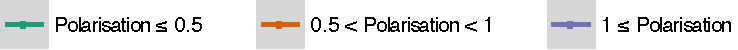
\includegraphics[width=90mm]{Graphics/legend_pol.pdf}
	\includegraphics[width=\textwidth]{Graphics/fig611a.pdf}
	\caption{Mean eccentricity for \emph{maxcov-inductor} model.}
	\label{fig:eccentricity_mi}
	\Fignote{Uses Monte Carlo parameterisation method, the \emph{ensemble average}, and is executed with 500 runs, 50 repetitions and 1000 burn-in iterations. Estimates smoothed using LOESS method.}
\end{figure}

The \emph{maxcov-inductor} and \emph{maxcov} firms locate at similar distances to the ideal point of all consumers, for all degrees of polarisation between the subpopulation. With a high degree of polarisation, mean eccentricity increases as the number of firms in the market increase (see figure~\ref{fig:eccentricity_mi}). Mean eccentricity tops with around seven firms in the market, and thereafter the mean distance of firms to the average ideal point of consumers remains at approximately 1.2 standard deviations. Although this was also observable in the \emph{maxcov} model (figure~\ref{fig:eccentricity_maxcov}), it is slightly clearer in the \emph{maxcov-inductor} model. Recall that \emph{maxcov} firms tend to split into two crowds when the consumer distribution is bimodal and asymmetry. Each crowd locates close to the peak of a subpopulation, and thus far from the average ideal point of all consumers. Consequently the mean distance to the ideal point increases as the number of firms increase. The firms in each crowd compete with one another and compete less with firms in the other crowd. With less than eight firms in the market firms are unlikely to switch its location from one crowd to the other. As the number of firms increase beyond seven firms the probability that a firm switches crowds increases. The decrease in mean eccentricity is due to firms moving between the peaks of the subpopulation, and thus temporarily locating closer to the average ideal points of all consumers. This also seems to indicate a limit as to how many firms the crowds can sustain, before firms from different crowds start to compete more directly with one another.

\begin{figure}[hb!]
	\caption{Trajectory plots for four firms in market with highly polarised subpopulation ($\mu=1.5$) and where left subpopulation is half as large as right subpopulations ($n_l/n_r = 1.5$). The black cross indicates the mean ideal point of all consumers.}
	\centering
	\begin{subfigure}[t]{0.485\textwidth}
		\includegraphics[width=\textwidth]{Graphics/figm_maxcov.pdf}
		\caption{Location of four \emph{maxcov}-firms after 155 iterations, where the lines show the location in the four preceding iterations. The two centre firms oscillate in opposite direction of each other.}
		\label{fig:four_maxcov}
	\end{subfigure}
	~
	\begin{subfigure}[t]{0.485\textwidth}
		\includegraphics[width=\textwidth]{Graphics/figm_maxcov-inductor.pdf}
		\caption{Location of four \emph{maxcov—inductor} firms after 1007 iterations, where the lines show the location in the six preceding iterations. The three firms on the left form a triangular configuration.}
		\label{fig:four_mi}
	\end{subfigure}
	\label{fig:four}
\end{figure}

Although estimated mean eccentricity is quite similar in the \emph{maxcov} and \emph{maxcov-inductor} model, there are slight differences in how the firms choose to locate. This is perhaps best illustrated by looking at an example with four firms in a highly polarised market ($\mu=1.5$). When subpopulations are equally large ($n_l/n_r = 1$) then two peripheral firms locate close to the peaks of each subpopulation, while the two centre firms oscillate left and right in opposite direction of each other (example of such oscillation in figure~\ref{fig:four_maxcov}). When the left subpopulation is twice as large as the right, the left peripheral firm locates close the peak of its subpopulation, while the three remaining firms locate close the peak of the left subpopulation in a triangular configuration (example in figure~\ref{fig:four_mi}). And so, increasing the relative size of the left subpopulation shifts the locations of the centre firms further left. At some critical relative size the location of the centre firms comes sufficiently close to the peak of the left subpopulation, and the centre firms switch from oscillation left-right and into the triangular configuration. These location behaviours are observed in both the \emph{maxcov} and \emph{maxcov-inductor} model. However peripheral \emph{maxcov-inductor} firms observe and predict the oscillation of the centre firms, and in response move closer to the centre. While centre firms shift further left to counterbalance the invasive peripheral firms, increasing the likelihood of the triangular configuration. This implies that the \emph{maxcov} model requires more uneven subpopulations, before the switch from oscillation to triangular configuration takes place, compared to the \emph{maxcov-inductor} model. In figure~\ref{fig:four}, for each of the two models, we plot the trajectories of four firms with $\mu=1.5$ and $n_l/n_r = 1.5$. When the left subpopulation is half as large as the right, the centre firms in the \emph{maxcov} model still exhibits oscillation, while three \emph{maxcov-inductor} firms locate in the triangle configuration, with the left peripheral firm located close to the peak of the left subpopulation. We are observing how predictions lead to strategic considerations that ultimately influence the location of firms. Similar type of behaviour is also observed when the number of firms is not four. However these case are harder to describe, since there are not just two different location configurations, but often many different configurations. Predictions do not lead to new location configurations, but they affect the circumstance that lead to specific configuration.

\begin{figure}[ht!]
	\centering
	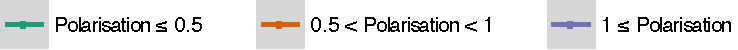
\includegraphics[width=90mm]{Graphics/legend_pol.pdf}
	\includegraphics[width=\textwidth]{Graphics/fig612a.pdf}
	\caption{Effective number of firms (ENP) for \emph{maxcov-inductor} model.}
	\label{fig:enp_mi}
\end{figure}

Comparing the \emph{effective number of firms} (ENP) in the \emph{maxcov-inductor} model (figure~\ref{fig:enp_mi}) to the \emph{maxcov} model (figure~\ref{fig:enp_maxcov})  reveals similar ENP with less than eight firms in the market or with a medium degree of polarisation. However with more than seven firms in the market and with a low or high degree of polarisation the ENP is higher in the \emph{maxcov-inductor} model. In these cases the fraction of consumers that each firm captures is more evenly distributed than in the \emph{maxcov} model. 

\begin{figure}[hb!]
	\caption{Trajectory plots for twelve firms. The top panels show the \emph{maxcov} model, where dots indicate the location of the firm after 160 iterations. The bottom panels show the \emph{maxcov-inductor} model, where dots indicate the location after 1010 iterations. The coloured lines show the location in the ten preceding iterations. The black lines are market boundaries after respectively 160 and 1010 iterations.}
	\centering
	
	\begin{subfigure}[t]{0.485\textwidth}
		\includegraphics[width=\textwidth]{Graphics/figm_cmu.pdf}
		\caption{\emph{Maxcov} firms in market with no polarisation ($\mu=0$, $n_r/n_l = 1$). Six of the firms have clustered at the centre of the market.}
		\label{fig:twelve_uni_maxcov}
	\end{subfigure}
	~
	\begin{subfigure}[t]{0.485\textwidth}
		\includegraphics[width=\textwidth]{Graphics/figm_cmb.pdf}
		\caption{\emph{Maxcov} firms in market with high polarisation and uneven sized subpopulations ($\mu=1.5$, $n_r/n_l = 2$). Five of the firms have clustered near the peak of the left subpopulation.}
		\label{fig:twelve_bi_maxcov}
	\end{subfigure}
	
	\begin{subfigure}[t]{0.485\textwidth}
		\includegraphics[width=\textwidth]{Graphics/figm_cmiu.pdf}
		\caption{\emph{Maxcov-inductor} firms in market with no polarisation ($\mu=0$, $n_r/n_l = 1$). No clustering of firms.}
		\label{fig:twelve_uni_mi}
	\end{subfigure}
	~
	\begin{subfigure}[t]{0.485\textwidth}
		\includegraphics[width=\textwidth]{Graphics/figm_cmib.pdf}
		\caption{\emph{Maxcov-inductor} firms in market with high polarisation and uneven sized subpopulations ($\mu=1.5$, $n_r/n_l = 2$). No clustering of firms at iteration 1010. The red firm located at the peak of the left subpopulation previously paired with another firm, but only temporarily.}
		\label{fig:twelve_bi_mi}
	\end{subfigure}
	
	\label{fig:twelve}
\end{figure}

In the \emph{maxcov} model with many firms and a low degree of polarisation, a handful of firms will cluster together at the same location, as seen in figure~\ref{fig:twelve_uni_maxcov}. The clustered firms move in tandem. Each of the clustered firms assume that the other firms remain at their current position, and given this relocates to maximise its market share. However all the other firms in the cluster make the same decision, and they all end up at the same location. Once a cluster of firms is formed, it sometimes absorbs additional firms, but seldomly breaks apart. Similarly with a high degree of polarisation and uneven sized subpopulations, see figure~\ref{fig:twelve_bi_maxcov}. This reduces the ENP in the \emph{maxcov} model with many firms, since the clustered firms compete for the same customers reducing their average market share. The clustering of \emph{maxcov} firms in the models with low or high degrees of polarisation occurs, because there is a high concentration of consumers around only one or two points. Competition for these high density areas forces firms closer together and clusters emerge. In the \emph{maxcov-inductor} model two firms may temporarily pair up, but any pairing of firms is short-lived and eventually breaks up, see figure~\ref{fig:twelve_uni_mi} and~\ref{fig:twelve_bi_mi}. In turn, the long-run share of customers is more evenly distributed among firms and we observe a higher ENP. One or both of the paired firms will predict the future location of its competitor and distance itself to increase its share of the market. With a medium degree of polarisation, clustering and pairing of firms is short-lived in both models. There is a non-neglige number of consumers with ideal points in between the peaks of the distribution function. Consumers are not just concentrated around one or two points, but the density of consumers is spread over a larger area. Competition no longer forces firms together which eliminates the clustering of firms.

The difference in mean representation between the \emph{maxcov} and \emph{maxcov-inductor} model is minuscule. The mean representation plot for the \emph{maxcov-inductor} model is therefore not included in the main text (see \ref{app:representation_mi}).

From the comparison above we learn that introducing firms with the ability to forecast the future location of competing firms has a limited effect on the how far away firms locate from the average ideal point of all consumers. This distance is largely determined by the method with which the firm determines its optimal location, in this case the firm locates in the Delaunay triangle that encompasses most consumers. Forecast however play an important role in shaping the location behaviour of firms in cases with oscillation. We see that \emph{maxcov-inductor} firms observe the oscillation of competing firms and uses this information to form its predictions. This precludes the most rudimentary oscillation patterns. Oscillation does not completely disappear with the introduction of \emph{maxcov-inductor} firms. In this paper firms are only able to recognise periodic oscillation with period 2. That is firms only use information about the autocorrelation between two consecutive periods. If firms were also able to recognise oscillation with a higher period, it would likely reduce oscillation even further. Furthermore we learn that several \emph{maxcov-inductor} firms are unlikely to cluster at the same location. Two firms may pair up, but this pairing is short-lived. One or both firms will anticipate the future movement of the other firm, and realise that it can increase its share of the market by distancing itself.

\subsubsection{Maxcov-inductor-GA model}

We extend the decision rule further. \emph{Maxcov-inductor-GA} firms locate in the Delaunay triangle that maximises its share. The firms use \emph{inductive reasoning} to forecast the future location of competing firms. And the firms gradually discard poorly performing hypotheses, and form new hypotheses using a Generic Algorithm. Thus hypotheses are endogenously formed.

\begin{figure}[ht!]
	\centering
	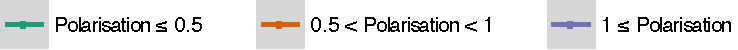
\includegraphics[width=90mm]{Graphics/legend_pol.pdf}
	\includegraphics[width=\textwidth]{Graphics/fig621a.pdf}
	\caption{Mean eccentricity for \emph{maxcov-inductor-GA} model.}
	\label{fig:eccentricity_miga}
	\Fignote{Uses Monte Carlo parameterisation method, the \emph{ensemble average}, and is executed with 500 runs, 50 repetitions and 2,500 burn-in iterations. Generic algorithm runs every 50th iterations. Estimates smoothed using LOESS method.}
\end{figure}

Once again we see very little change in the mean distance to the ideal point of all consumers with a low and medium degree of polarisation. \emph{Maxcov-inductor-GA} firms locate in the Delaunay triangle that maximises its share. This is the decisive factor in determining the mean distance to the ideal point. With a high degree of polarisation between the two subpopulations mean eccentricity is significantly lower in a market with five firms compared with the \emph{maxcov-inductor} model.

\begin{figure}[hb!]
	\centering
	\caption{Trajectory plot for five \emph{maxcov-inductor-GA} firms at different iteration intervals ($\mu=1.3$ and $n_l/n_r=1.5$). The dots indicate the location after respective 270, 320 and 2,500 iterations and the lines indicate the location in preceding iterations. The black cross indicates the average ideal point of all consumers.}
	
	\begin{subfigure}[t]{0.315\textwidth}
		\centering
		\includegraphics[width=\textwidth, trim={6mm 0 2mm 0}]{Graphics/fig6m_miga1.pdf}
		\caption{Three-two split.}
		\label{fig:five32}
	\end{subfigure}
	~
	\begin{subfigure}[t]{0.315\textwidth}
		\centering
		\includegraphics[width=\textwidth, trim={6mm 0 2mm 0}]{Graphics/fig6m_miga2.pdf}
		\caption{Transition interval.}
		\label{fig:fivetransition}
	\end{subfigure}
	~
	\begin{subfigure}[t]{0.315\textwidth}
		\centering
		\includegraphics[width=\textwidth, trim={6mm 0 2mm 0}]{Graphics/fig6m_miga3.pdf}
		\caption{Four-one split.}
		\label{fig:five41}
	\end{subfigure}
	
	\label{fig:five}
\end{figure}

As mentioned earlier firms tend to split into two crowds when the there is a high degree of polarisation between the mean ideal points of the two subpopulations. With five firms and the degree of polarisation close to 1.5, the firms tend to locate in a three-two split. When the degree of polarisation is close to 1 and the distribution is sufficiently asymmetric ($n_l/n_r$ not too close to 1), then the split tends to be four-one. This is the case in both the \emph{maxcov-inductor} and \emph{maxcov-inductor-GA} model. However the \emph{maxcov-inductor-GA} model requires less polarisation among the subpopulations for the four-one split to occur. In figure~\ref{fig:five} we plot the location of five \emph{maxcov-inductor-GA} firms for $mu = 1.3$ and $n_l/n_r = 1.5$. The firms quickly converge to the three-two split, but this location configuration is not sustained and after 270 iterations the firms transition into a four-one split. For comparison we re-execute the model with the same initial positions and the same set of endowed \emph{condition/forecast} rules, but where firms use the \emph{maxcov-inductor} decision rule instead of \emph{maxcov-inductor-GA}. The \emph{maxcov-inductor} firms maintain the three-two split also after 270 iterations and locate as in figure~\ref{fig:five32}. This explains why we observe a lower mean eccentricity in the \emph{maxcov-inductor-GA} model with five firms compared to the \emph{maxcov-inductor} model. With a four-one split the firms locate closer to the average ideal point of consumers than firms that locate in a three-two split.

\begin{figure}[hb!]
	\caption{Average forecast error variance of all the activated \emph{condition/forecast} rules of the firms.}
	\centering
	
	\begin{subfigure}[t]{0.485\textwidth}
		\includegraphics[width=\textwidth, trim={4mm 0 0 0}]{Graphics/fig6a_mi_same.pdf}
		\caption{Five \emph{maxcov-inductor} firms with the same initial position and set of endowed \emph{condition/forecast} rules.}
		\label{fig:accuracy_maxcov}
	\end{subfigure}
	~
	\begin{subfigure}[t]{0.485\textwidth}
		\includegraphics[width=\textwidth, trim={4mm 0 0 0}]{Graphics/fig6a_miga.pdf}
		\caption{Five \emph{maxcov-inductor-GA} firms. Every 50th iteration the firms discard and replaces the 20\% poorest performing \emph{condition/forecast} rules. The transition interval is highlighted.}
		\label{fig:accuracy_mi}
	\end{subfigure}
	
	\label{fig:accuracy}
\end{figure}

Furthermore we can compare the accuracy of the two cases. The \emph{maxcov-inductor-GA} firms replaces the 20\% worst performing hypotheses every 50th iteration, while the \emph{maxcov-inductor} firm uses the same set of $M$ hypotheses indefinitely. In figure~\ref{fig:accuracy} we plot the average forecast error variance of all the \emph{condition/forecast} rules for each the firm at each iteration. We disregard \emph{condition/forecast} rules that have a forecast error variance of zero, and thus have not previously been active. A low forecast error variance indicates that the hypothesis provided accurate predictions in the past. We focus on the first 500 iterations. For the first 50 iterations the forecast error variance is the same in both cases, since the firms make predictions using their endowed set of hypotheses. In the \emph{maxcov} model the average forecast error variance increases steadily, but at a steadily decreasing rate, as firms learn which hypothesis provide the most accurate predictions, see figure~\ref{fig:accuracy_maxcov}. Firms learn through experience. This is also the case in the \emph{maxcov-inductor-GA} model, but in additions firms learn through adaption. Discarding poorly performing hypotheses and replacing them with new hypotheses that are based on the best performing hypotheses significantly increases the accuracy, as seen in figure~\ref{fig:accuracy_mi}. After 270 iterations the firms have discovered a sufficiently accurate location pattern of their competing firms, allowing the firms to move from the three-two split to the four-one split. Notice that the three firms that move furthest in the transition interval are not simultaneously experiencing an increase in their average forecast error variance. The predictions they make during this transition are at least as precise as previous predictions. Thus the transition cannot be attributed to synchronised and systematic break down in forecasts, but rather the transition is the result of a deliberate and calculated response to the predicted future locations of competing firms. These are strategic moves. While the two other firms experience an increasing average forecast error variance during the transition, they quickly adapt to the environmental change. And we see that shortly after the transition the firms are quite similar in terms of the accuracy of their hypotheses.

\begin{figure}[ht!]
	\centering
	\includegraphics[width=90mm]{Graphics/legend_pol.pdf}
	\includegraphics[width=\textwidth]{Graphics/fig622a.pdf}
	\caption{Effective number of firms (ENP) for \emph{maxcov-inductor-GA} model.}
	\label{fig:enp_miga}
\end{figure}

The effective number of firms (ENP) is largely unaffected by the extension of the decision rule. In the model with five firms, where the four-one split is more likely, results in a lower ENP, since the single firm captures the entire right side of the market for itself. Examining the market share of each firm over time reveals differences in terms of the long-run competitive advantage one firm may have over its competitors. This is best illustrated in a market with three firms, by comparing the \emph{maxcov}, the \emph{maxcov-inductor} and the \emph{maxcov-inductor-GA} model. For each model we plot the market share across time in a market with a highly polarised and uneven sized subpopulations ($\mu=1.5$ and $n_l/n_r = 2$). See figure~\ref{fig:share}. 

\begin{figure}[hb!]
	\centering
	\caption{Share of market with three firms, $\mu = 1.5$ and $n_l/n_r = 2$. Red line is the firm located at the right peak. While the blue and green line are the two firms located close to the left peak.}
	
	\begin{subfigure}[t]{\textwidth}
		\centering
		\includegraphics[width=\textwidth, trim={4mm 3mm 4mm 6mm}]{Graphics/fig5s_m.pdf}
		\caption{\emph{Maxcov} model.}
		\label{fig:share_maxcov}
	\end{subfigure}
	
	\begin{subfigure}[t]{\textwidth}
		\centering
		\includegraphics[width=\textwidth, trim={4mm 3mm 4mm 6mm}]{Graphics/fig5s_mi.pdf}
		\caption{\emph{Maxcov-inductor} model.}
		\label{fig:share_mi}
	\end{subfigure}
	
	\begin{subfigure}[t]{\textwidth}
		\centering
		\includegraphics[width=\textwidth, trim={4mm 3mm 4mm 6mm}]{Graphics/fig5s_miga.pdf}
		\caption{\emph{Maxcov-inductor-GA} model.}
		\label{fig:share_miga}
	\end{subfigure}
	
	\label{fig:share}
\end{figure}

In the \emph{maxcov} model, after the initial burn-in periods, the location of the firms lock in. One firm locates close to the right peak of the distribution function, while the two other firms locate around the left peak. The location of the right firm is consistent across different initial locations, while the location configuration, which the two firms on the left lock into vary depending on the initial position of firms. Additionally the two firms on the left often oscillate. The firm on the right captures 1/3 of the market. One of the firms on the left captures a slightly larger share, and the other a slightly lower share. While our estimate of the ENP is independent of the initial position of firms, the initial position determines how each firm ranks in term of market share. It is evident from figure~\ref{fig:share_maxcov}, that certain initial positions gives one firm a clear long-run competitive advantage over its competitors in the \emph{maxcov} model. 

In the \emph{maxcov-inductor} model firms predict the future location of competing firms, using the hypotheses that match the current state and proved most accurate in the past. After several dozen burn-in iterations the firm on the right once again locates close the right peak and captures 1/3 of the market. The two firms on the left will not immediately lock in, but switch between different location configurations. The ranking in terms of market share changes when the two firms switch between configurations\footnote{These configurations are the same as those that arose, when using different initial positions, in the \emph{maxcov} model.}. The firms do not immediately lock in, since firms are able to predict and respond to the future location of competing firms, such as oscillation. Over time the firms learn which of their hypotheses give the most reliable predictions. And the firm often ends up using a limited set of hypotheses, see figure~\ref{fig:cf}. The two firms on the left lock into a specific configuration or a specific few configurations, once all firms converge to using a limited set of hypotheses. Once the firms lock in, so does their share of the market, as seen in figure~\ref{fig:share_mi}. The initial position of the firm does not by itself create a long-run competitive advantage in the \emph{maxcov-inductor} model. Instead it is a combination of initial position and the set of hypotheses which the firms is endowed with, that can give the firm a long-run competitive advantage. While the firm is able to update the accuracy of each hypothesis, the conditions and forecast values remain fixed. If a firm is endowed with a set of poorly performing hypotheses, then the firm is unlikely to capture more than 1/3 of the market in the long-run. 

\begin{figure}[ht!]
	\centering
	\includegraphics[width=\textwidth]{Graphics/fig5cf_mi.pdf}
	\caption{The \emph{condition/forecast} rule used at each iteration by each of the three \emph{maxcov-inductor} firms to forecast the future location of competing firms. After approximately 200 iterations all firms use a limited set of \emph{condition/forecast} rules. After approximately 400 iterations the set does not change. The firm on the right is red, the two firms on the left are green and blue respectively.}
	\label{fig:cf}
\end{figure}

In the \emph{maxcov-inductor-GA} model the two firms on the left never lock in, but continue to switch between the different location configurations. \TODO{LOCATION CONFIGURATIONS.} The firms may temporarily get stuck in a specific configuration, where all firms use a limit set of hypotheses, but eventually the firms form new hypotheses that change how the firms locate. The set of hypotheses which the firm is endowed with does not give the firm a long-run competitive advantage over its competitors. Instead there will be prolonged periods where one of the two firms on the left capture more than 1/3 of the market, followed by periods where the reverse is true, as seen in figure~\ref{fig:share_miga}. This highlights how one firm may use tactics that are superior to its competitors and how competing firms gradually learn and develop counteracting responses. The \emph{maxcov-inductor-GA} firm continuously adapts to changes in its environment. This type of behaviour is not unique to a market with three firms and highly polarised and uneven sized subpopulations. The same is true with a different number of firms in the market and different parameter values\footnote{The polarised and uneven market with three firms contains a lot of different location configurations while the low number of firms makes it easier to describe. And so we used this for the basis of the example. With two or four firms in the market there are only a few location configurations, all of which are fairly stable, and so the described behaviour is less pronounced since there is less changes to the environment of the firm.}. 

\begin{figure}[ht!]
	\centering
	\includegraphics[width=90mm]{Graphics/legend_pol.pdf}
	\includegraphics[width=\textwidth]{Graphics/fig623a.pdf}
	\caption{Mean representation for \emph{maxcov-inductor-GA} model.}
	\label{fig:representation_miga}
\end{figure}

The mean representation in the \emph{maxcov-inductor-GA} model is almost identical to the \emph{maxcov} and \emph{maxcov-inductor} model, as seen in figure~\ref{fig:representation_miga}.


\section{Conclusion}

This paper set out to reintroduce foresight and thus strategic consideration into the competitive location model. Something that has thus far been missing from the agent-based models. The paper argues why it is unreasonable to assume that firms use \emph{deductive reasoning} to deduce their optimal location. Instead we argue that firms derive principles and conclusions from observations and viewing conclusions as probable, rather than certain, i.e. firms use \emph{inductive reasoning}. The firms possess numerous hypotheses, each relevant to specific set of situations. Hypotheses are updated in response to new information or observations that falsifies the currently held hypotheses. The firms predict the future location of competing firms, using the hypothesis viewed as most probable in the given situation. When a firm chooses its own location it takes the future location of competing firms into account. The firm acts strategically, and is no longer oblivious to the simultaneous relocation of competing firms.

The model in this paper encompasses the ``natural'' setting of competitive product differentiation or location differentiation. That is a setting with few firms in the market that is not necessarily restricted to a single dimension and where the distribution of consumer preferences might be asymmetric and multimodal. The conclusions from the previous literature on competitive location models mainly concern one dimensional markets or duopolies. Yet in most markets more than two firms compete, and they often choose along several product characteristics not just one. While it is convenient to assume that consumers are uniformly distributed, this assumption is highly unrealistic. The case where the preference of all consumers is uncorrelated must be considered a special case. More generally consumers are likely to lump together in subpopulations. Possibly due to social interactions among consumers, such as desire for social conformity or other network effects. These subpopulations then give rise to an aggregated distribution of consumer preferences that is multimodal and quite possibly asymmetric.

Predictions by themselves have a limited effect on the overall location pattern of firms. We do not observe locations that are fundamentally different when using decision rules with foresight. The main driver in determining the location patterns is the method used by the firms to determine the optimal location given its predictions. In this paper the firms located in the Delaunay triangle with most consumers. While predictions do not affect the overall location pattern, they do influence specific location behaviours such as oscillation, clustering of firms, and it changes the probability of certain location patterns. In a market with many firms predictions lead the firms to capture a more even share of the market, namely because any pairing of firms is short lived. This is somewhat surprising given the fact that we introduce additional sources of heterogeneity for firms. In the models with foresight firms are also heterogeneous in terms of their expectation model and knowledge.

In the paper we also consider the social welfare of consumers. The interacting effect of firms competing for consumers seems to results in locations that are more or less on par with the social optimal location (except in the cases with less than four \emph{hunter} firms and a bimodal distribution). This is a quite striking result considering the conclusions of earlier papers. In the line market, the \emph{principle of local clustering}, lead firms to locate far from the social optimal locations. And in the two-dimensional Hotelling model with a uniform distribution of consumers, the two firms locate at the centre, thus also far from the social optimum. The main reason that competition leads to more or less socially optimal locations in this paper is due to the assumed distribution function. We assume that each subpopulation follow a bivariate normal distribution with standard deviation (0.5, 0.5). This gives a high concentration of consumers around the peaks of the aggregated distribution function. Increasing the standard deviations would decrease the concentration of consumers around the peaks, and we would most likely observe a decrease in the average utility of consumers that would be more in line with previous papers. 

The paper is a first attempt at laying down the foundation for a competitive location model with foresight. There is still ample room for improvement and many possible extensions. An obvious extension is entry and exit of firms such that the number of firms is endogenously determined. Similarly incorporating price competition into the model seems to be a natural next step. The lack of methods for finding the optimal location meant that in all the \emph{maxcov} decision rules used a rough approximation. Developing new techniques for finding the optimal location of new entrants in the market, as well as the optimal location of existing firms, would be of benefit to the models in this paper, and the field in general.


% Appendix
\newpage
\begingroup
\appendix

\section{Model overview}
\label{app:overview}

The following subsection contains an overview of the various models. In addition arguments for the underlying process of a \emph{run} is provided. We abbreviate time-homogenous Markov chain as THMC

\subsubsection*{All-sticker:}
The underlying process is a non-ergodic deterministic THMC. The firms never move so the initial state space distribution, $\pi_0$, is stationary and solves $\pi_{t+1} = \pi_t$. The process is fixed in a single state, which depends the initial position of the firm, thus the process is non-ergodic.

\subsubsection*{All-aggregator:}
The underlying process is a non-ergodic deterministic THMC. The process does not contain a random component, since firms always locating at the centroid of their current market. When all firms use the \emph{aggregator}-rule then a \emph{repetition} is an implementation of the Lloyd-algorithm, which always leads to a \emph{centroidal Voronoi tessellation} (CVT). Thus the process converges to a single state. There is no guarantee that the CVT is unique, a different initial position of the firms might result in a different CVT, which implies that the process is \emph{non-ergodic}.

\subsubsection*{All-hunter:}
The underlying process is a ergodic stochastic THMC. Whenever a \emph{hunter} firm experiences a decrease in its market share, the firm turns around and heads in a randomly drawn opposite direction. This random component, makes the underlying process \emph{ergodic}. With a random component every state in the state space has strictly positive probability of being reached in a finite number of iterations. Thus the process, figuratively speaking, avoids getting stuck in a blind alley. Eventually the process will converge to its unique distribution vector, $\pi_\infty$. In the model with a symmetric distribution of consumers the \emph{time average} provides a representative estimate of $\psi$, i.e. for all output variables the R-hat statistic is below 1.05. The model with an asymmetric and bimodal distribution of consumers contains two additional free parameters. In this model we find that several R-hat statistics that are above 1.05 — even when executing the test repetitions with 20,000 iterations. For this model we conclude that the \emph{time average} does not provides a representative estimate of $\psi$, and we instead use the \emph{ensemble average}. 

\subsubsection*{All-maxcov:}
The underlying process is a non-ergodic deterministic THMC. The process does not contain a random component, since firms always locating at the centroid of the largest Delaunay triangle. Unlike the other deterministic THMC, this process does not converge to a single state, since firms often oscillate between different locations. Furthermore we observe that different initial locations of firms converge to different locations (or converge to different oscillation patterns, i.e. different sets of locations). So the process is \emph{non-ergodic}, i.e. the stationary state space distribution, $\pi_\infty$ depends on the initial state space distribution, $\pi_0$. The paper assumes that firms oscillate between a few locations that are not too far apart. It also assumes different initial position only lead to minor differences in the location which firms converge to. With these assumptions in mind we use the \emph{ensemble average} to estimate $\psi$ (see discussion in subsection~\ref{sec:oscmaxcov}).

\subsubsection*{All-maxcovrnd:}
The underlying process is a ergodic stochastic THMC. The process contains a random component, since the speed parameter is randomly drawn. Instead of the firm moving 0.1 standard deviations, the move is drawn uniformly random from the range $[0, 0.2]$. This insures that every state in the state space has strictly positive probability of being reached in a finite number of iterations. The process will eventually converge to the unique distribution vector, $\pi_\infty$. Every \emph{stochastic THMC} with a finite state space is \emph{ergodic} \citep[chapter~4, p.~64]{Laver_Sergenti_2011}. We estimate $\psi$ using the \emph{ensemble average}, and compare the results with the \emph{all-maxcov} model to see if our assumption in that model regarding oscillation and the steady state distributions are reasonable.

\subsubsection*{Maxcov-inductor:}
The underlying process does not fulfil the Markov property. The \emph{trending bits} and \emph{oscillation bits} calculate respectively the moving average and the autocorrelation using the location history of the firm. And so the probability of the future state will depend on past states, and only the current state, which violates the Markov property. Furthermore since the firm updates the accuracy of it hypotheses the \emph{transition probability} is not stationary. The \emph{transition probability} depends on the experience of the firm, and since the experience evolves so will the \emph{transition probabilities}. Even without the \emph{trending bits} and \emph{oscillation bits} the underlying process would not constitute a THMC. While it has not yet been proven if the \emph{ensemble average} provides a representative estimate of $\psi$, this is none the less the method used in previous papers, and will therefore all be the method employed in this paper.

\subsubsection*{Maxcov-inductor-GA:}
The underlying process does not fulfil the Markov property either. The reason is the same as in the \emph{maxcov-inductor} model. The genetic algorithm which the firm uses to construct new hypotheses with random mutation and crossover, means that there is a random competent in the underlying process.

\section{Maxcovrnd decision rule}
\label{app:maxcovrnd}

To test our assumptions and see if it is reasonable to use the \emph{ensemble average} to estimate $\psi$ in the \emph{maxcov} model we create a new decision rule \emph{maxcovrnd}. Firms using the \emph{maxcovrnd} decision rule will not move 0.1 standard deviations, but uniformly random draw the speed parameter from the range $[0, 0.2]$. On average the two decision rules have the same speed parameter. By randomly drawing the speed parameter we introduce a random component into the process. In the model where all firms use the \emph{maxcovrnd} rule, the random component in the process, insures that the \emph{ensemble average} provides a representative estimate of $\psi$. We execute both models and estimate using the \emph{ensemble average}. If the two models provide similar estimates, then firms only oscillate between a few similar locations in the \emph{maxcov} model, and different initial position only leads to slightly differences in the locations which firms converge to. If this is the case we conclude that our assumptions are reasonable, and we feel confident using the \emph{ensemble average} in the \emph{maxcov} model. Figures~\ref{fig:maxcovrnd} and~\ref{fig:asys_maxcovrnd} plots the estimates from the models with respective a symmetric unimodal distribution and an asymmetric bimodal distribution of consumers. The difference between the \emph{maxcov} and \emph{maxcovrnd} model is minuscule.

\begin{figure}[ht!]
	\centering
	\caption{Estimates from market with symmetric and unimodal distribution of consumers ($\mu = 0$ and $n_l/n_r = 1$). Solid lines is \emph{maxcov} model and the dashed line is the \emph{maxcovrnd} model.}
	\includegraphics[width=42.5mm]{Graphics/legend_maxcovrnd.pdf}

	\begin{subfigure}[t]{0.315\textwidth}
		\centering
		\includegraphics[width=\textwidth, trim={4mm 0 0 0}]{Graphics/figA11.pdf}
		\caption{Mean eccentricity.}
		\label{fig:eccentricity_maxcovrnd}
	\end{subfigure}
	~
	\begin{subfigure}[t]{0.315\textwidth}
		\centering
		\includegraphics[width=\textwidth, trim={4mm 0 0 0}]{Graphics/figA12.pdf}
		\caption{Effective number of firms.}
		\label{fig:enp_maxcovrnd}
	\end{subfigure}
	~
	\begin{subfigure}[t]{0.315\textwidth}
		\centering
		\includegraphics[width=\textwidth, trim={4mm 0 0 0}]{Graphics/figA13.pdf}
		\caption{Mean representation.}
		\label{fig:representation_maxcovrnd}
	\end{subfigure}

	\label{fig:maxcovrnd}
	\Fignote{Both models use grid sweep method. Each model executes 11 runs, 1,000 repetitions, and 99 burn-in iterations.}
\end{figure}

\begin{figure}[ht!]
	\centering
	\caption{Estimates from market with asymmetric and bimodal distribution of consumers ($\mu \in [0,1.5]$ and $n_l/n_r \in [1,2]$). Solid lines is \emph{maxcov} model and the dashed line is the \emph{maxcovrnd} model.}
	\includegraphics[width=127.5mm]{Graphics/legend_maxcovrnd_pol.pdf}
	
	\begin{subfigure}[t]{0.315\textwidth}
		\centering
		\includegraphics[width=\textwidth, trim={8mm 0 0 0}]{Graphics/figA21.pdf}
		\caption{Mean eccentricity.}
		\label{fig:asys_eccentricity_maxcovrnd}
	\end{subfigure}
	~
	\begin{subfigure}[t]{0.315\textwidth}
		\centering
		\includegraphics[width=\textwidth, trim={8mm 0 0 0}]{Graphics/figA22.pdf}
		\caption{Effective number of firms.}
		\label{fig:asys_enp_maxcovrnd}
	\end{subfigure}
	~
	\begin{subfigure}[t]{0.315\textwidth}
		\centering
		\includegraphics[width=\textwidth, trim={8mm 0 0 0}]{Graphics/figA23.pdf}
		\caption{Mean representation.}
		\label{fig:asys_representation_maxcovrnd}
	\end{subfigure}

	\label{fig:asys_maxcovrnd}
	\Fignote{Both models use Monte Carlo parameterisation method, the \emph{ensemble average}, and is executed with 500 runs, 50 repetitions and 150 burn-in iterations. Estimates smoothed using LOESS method.}
\end{figure}

\section{Further details on condition/forecast rules}
\label{app:details}

This subsection provides further details — such as equations, parameter values and probability values — used in relation to the \emph{condition/forecast} rules and the genetic algorithm.

Each firm holds a set of $M$ hypotheses or \emph{condition/forecast} rules. While each hypothesis might only be relevant to a narrow set of situations, together the array of hypotheses cover a wide range of different situations. We follow \citet[chapter~3]{Arthur_2014} and set the number of hypotheses to one hundred, i.e. $M=100$.

\subsubsection*{Accuracy:}

The firm predicts the future location using the hypothesis it finds most probable given the current state of the competing firm. If the condition part of the rule is satisfied by the current state descriptor, $J_j$, of competing firm $j$, then that rule is said to be active. Several \emph{condition/forecast} rules may match the current state of competing firm $j$ and the firm uses the same set of $M$ \emph{condition/forecast} rules for all competing firms, so in any given iteration multiple \emph{condition/forecast} rules are likely to be active. The accuracy of all the active \emph{condition/forecast} rules is updated once the firms relocate and the actual location of each competing firm is revealed. The forecast error of each active rule is the difference between its predicted location and the actual location. To update the accuracy of \emph{condition/forecast} rules we use an inverse moving average of squared forecast errors \citep[chapter~3]{Arthur_2014}. We update the forecast error variance of a given active \emph{condition/forecast} rule $m$ at iteration $t$ using:

\begin{equation}
e^2_{t,i,m} = \alpha_a e^2_{t-1,i,m} + (1-\alpha_a) d\left( X_{t+1,j}, E_{t,i,m} [X_{t+1,j}] \right)^2
\end{equation}

where firm $i$ uses rule $m$ to make the forecast $E_{t,i,m} [X_{t+1,j}]$ about the future location of competing firm $j$. The actual future location of competing firm $j$ is $X_{t+1,j}$. The forecast error, $d(\cdot,\cdot)$, is the Euclidean distance between the actual and the predicted location. We assume that all firms use the same memory parameter $\alpha_a$ to update the accuracy. If the \emph{condition/forecast} rule $m$ is not active at iteration $t$, then the forecast error variance is unchanged: 

$$e^2_{t,i,m} = e^2_{t-1,i,m}$$

We choose to smooth out the accuracy and therefore set a high memory parameter; $\alpha_a = 74/75$. Thus new information has a relatively low impact on the accuracy of the \emph{condition/forecast} rule, and we avoid that one bad prediction suspends the future use of the rule.

\subsection{Genetic algorithm}
\label{app:gadetails}

Every $\tau$ number of iterations the firm discards the 20\% least fit \emph{condition/forecast} rules and replaces these with new \emph{condition/forecast} rules created using a genetic algorithm through a process of mutation and crossover of the non-discarded rules. We set choose a quick exploration rate and set $\tau = 50$.

\subsubsection*{Fitness:}

The fitness of each \emph{condition/forecast} rules is based on the accuracy and the specificity of the rule. The specificity of a rule is calculated as the number of ones and zeros in the condition part of the rule (i.e. all the \texttt{\#}'s are not counted). We calculate the fitness of rule $m$ at iteration $t$ using:

\begin{equation}
f_{t,i,m} = M - e^2_{t,i,m} - s_m c
\end{equation}

where firm $i$ hold rules $m$. The total number of \emph{condition/forecast} rules held by firm $i$ is $M$. This is constant and identical across firms, so the term can be left out. The forecast error variance of rule $m$ is $e^2_{t,i,m}$. The specificity of rule $m$ is $s_m$, and $c$ is the cost levied on the specificity. Inaccurate rules have a higher forecast error variance which reduces the fitness of the rule. A more specific rule also reduces the fitness of the rule. Thus accounting for the specificity of the rule creates a drift towards more generally applicable rules that fit a wider range of situations (i.e. rules with more \texttt{\#}'s in the condition). The condition consists of 13 positions and the average forecast error is below 0.1 so we set the cost of specificity to $c = 0.0005$ creating a slight drift towards more general rules.

\subsubsection*{Crossover:}
Each new hypothesis is based on two ``parent'' hypotheses. The pair of parent \emph{condition/forecast} rules are randomly selection from the set of non-discarded rules, i.e. the 80\% most fit \emph{condition/forecast} rules. A new \emph{condition/forecast} rule is created by either the mutation procedure or crossover procedure. For each new rule the procedure is randomly selected. The crossover procedure is selected with probability $p$, and mutation procedure with probability $1-p$. This paper follows \citet[chapter~3]{Arthur_2014} by using $p = 0.3$. With crossover the new \emph{condition/forecast} rule is a mix of both parents. The condition part is mixed by randomly selecting a donor parent for each of the 13 positions. Crossover of the forecast parameter values happens by either 1) component-wise crossover of each value, 2) using the weighted average of the parents or 3) randomly picking a parent that passes on all parameter values. The three methods are randomly selected with equal probability.

\subsubsection*{Mutation:}
With mutation the new hypothesis only inherits traits from the most fit of the two parents. Each position in the condition part is mutated with probability 0.03 and takes the value of the most fit parent with probability 0.97. The position is mutated by flipping its value. The probability that a \texttt{0} or a \texttt{1} is flipped to a \texttt{\#} is 2/3. The probability that \texttt{0} is flipped to \texttt{1}, or visa versa, is 1/3. The probability that a \texttt{\#} is flipped to a \texttt{1} or \texttt{0} is 1/3 respectively, where the remaining 1/3 is the probability that \texttt{\#} is not flipped. These flip-probabilities can also be written as a matrix:

\begin{equation}
P = \left[ {\begin{array}{*{20}{c}} 0&{\frac{1}{3}}&{\frac{2}{3}} \\ {\frac{1}{3}}&0&{\frac{2}{3}} \\ {\frac{1}{3}}&{\frac{1}{3}}&{\frac{1}{3}} \end{array}} \right]
\end{equation}

Taking the limit of $P^x$ for $x \to \infty$ reveals that the mutation of bits does not lead to a drift in the specificity of the rules:

\begin{equation}
\mathop {\lim }\limits_{x \to \infty } {P^x} = \left[ {\begin{array}{*{20}{c}} {0.25}&{0.25}&{0.5} \\ {0.25}&{0.25}&{0.5} \\ {0.25}&{0.25}&{0.5} \end{array}} \right]
\end{equation}

Repeatedly flipping a value in the condition will lead to a 50\% chance of it taking the value \texttt{0} or \texttt{1}, and 50\% chance of it taking the value \texttt{\#}. A steady drift in the specificity of the \emph{condition/forecast} rules occurs because we levy a positive cost, i.e. $c > 0$. The forecast parameter values are also mutated. Each value is either replaced or modified, each with probability 0.2. The forecast parameter takes the same value as the most fit parent with probability 0.6. If the value is replaced, then the new parameter value is drawn randomly from the same ranges as the initial parameter values (range of parameter values presented in subsection~\ref{sec:mi}). A modified value is equal to the value of the most fit parent, altered with a randomly drawn amount in the range $[-0.5\%, 0.5\%]$ times the length of the respective initial parameter range. For example let $A_1$ be the third forecast parameter value of the parent ($A_1$ has been drawn from the range $[0.99, 1.01]$ which has a length of 0.02) — if the randomly drawn amount is -0.5\%, then the new modified value becomes: $A_1 - 0.5\% \times 0.02 = A_1 - 0.0001$.

\section{Mean representation in maxcov-inductor model}
\label{app:representation_mi}

\begin{figure}[ht]
	\centering
	\includegraphics[width=90mm]{Graphics/legend_pol.pdf}
	\includegraphics[width=\textwidth]{Graphics/fig613a.pdf}
	\caption{Mean representation for \emph{maxcov-inductor} model.}
	\label{fig:representation_mi}
\end{figure}



\newpage
%% References
%\nocite{*}
\addcontentsline{toc}{section}{References}
%\section{References}
%\bibliographystyle{apalike-url}
\bibliographystyle{newapa-url}
\raggedright
\singlespacing
\bibliography{ALL.bib}

\end{document}